\chapter{Results and Discussion}
\label{Results}
This chapter covers different network and power usage patterns for the IoT devices in the testbed. First, Section \ref{swappingSwitch} informally compares the smart switches between devices to confirm that they are accurate enough for this research's purposes. Section \ref{General Analysis} covers smart speaker and streaming device network and power use while idle, in use, and during first boot. Section \ref{General Analysis} serves as precursory analysis to fingerprint devices and give example uses of the database and visualizer tool.

After general analysis, Section \ref{Power Analysis on Smart Speakers} shows how a power trace may highlight the presence of a user in their home. Sections \ref{sumPowerGraph} and \ref{sumPowerGraphWithNoise} cover summed power graphs of the smart speakers with and without noise from high power household devices. Finally, Section \ref{smartSpeakerComparisonSection} ends with a comparison between smart speakers for further general analysis.

When obtaining data, most of the packets are encrypted, so the data presented focuses on metadata such as size, protocol, source IP, and destination IP. For power analysis, we focus on the power used at each second.

\section{Swapping the Power Switch}
\label{swappingSwitch}
To check if the smart switch voltage readings are accurate, we swapped various devices with various power switches. Some examples are shown in Figures \ref{fig:swapEcho1Home}, \ref{fig:swapEufy1Echo1}, and \ref{fig:swapEufy1Home}. After swapping the switches, each device takes some time to start up, the colored boxes in Figures \ref{fig:swapEcho1Home}, \ref{fig:swapEufy1Echo1}, and \ref{fig:swapEufy1Home} highlight this time.

In every case, the traces swapped as we swapped the device connected to each smart switch. This informal sanity check confirmed that the power switches were precise enough to enable basic device comparisons.

\begin{figure}[H]
    \centering
    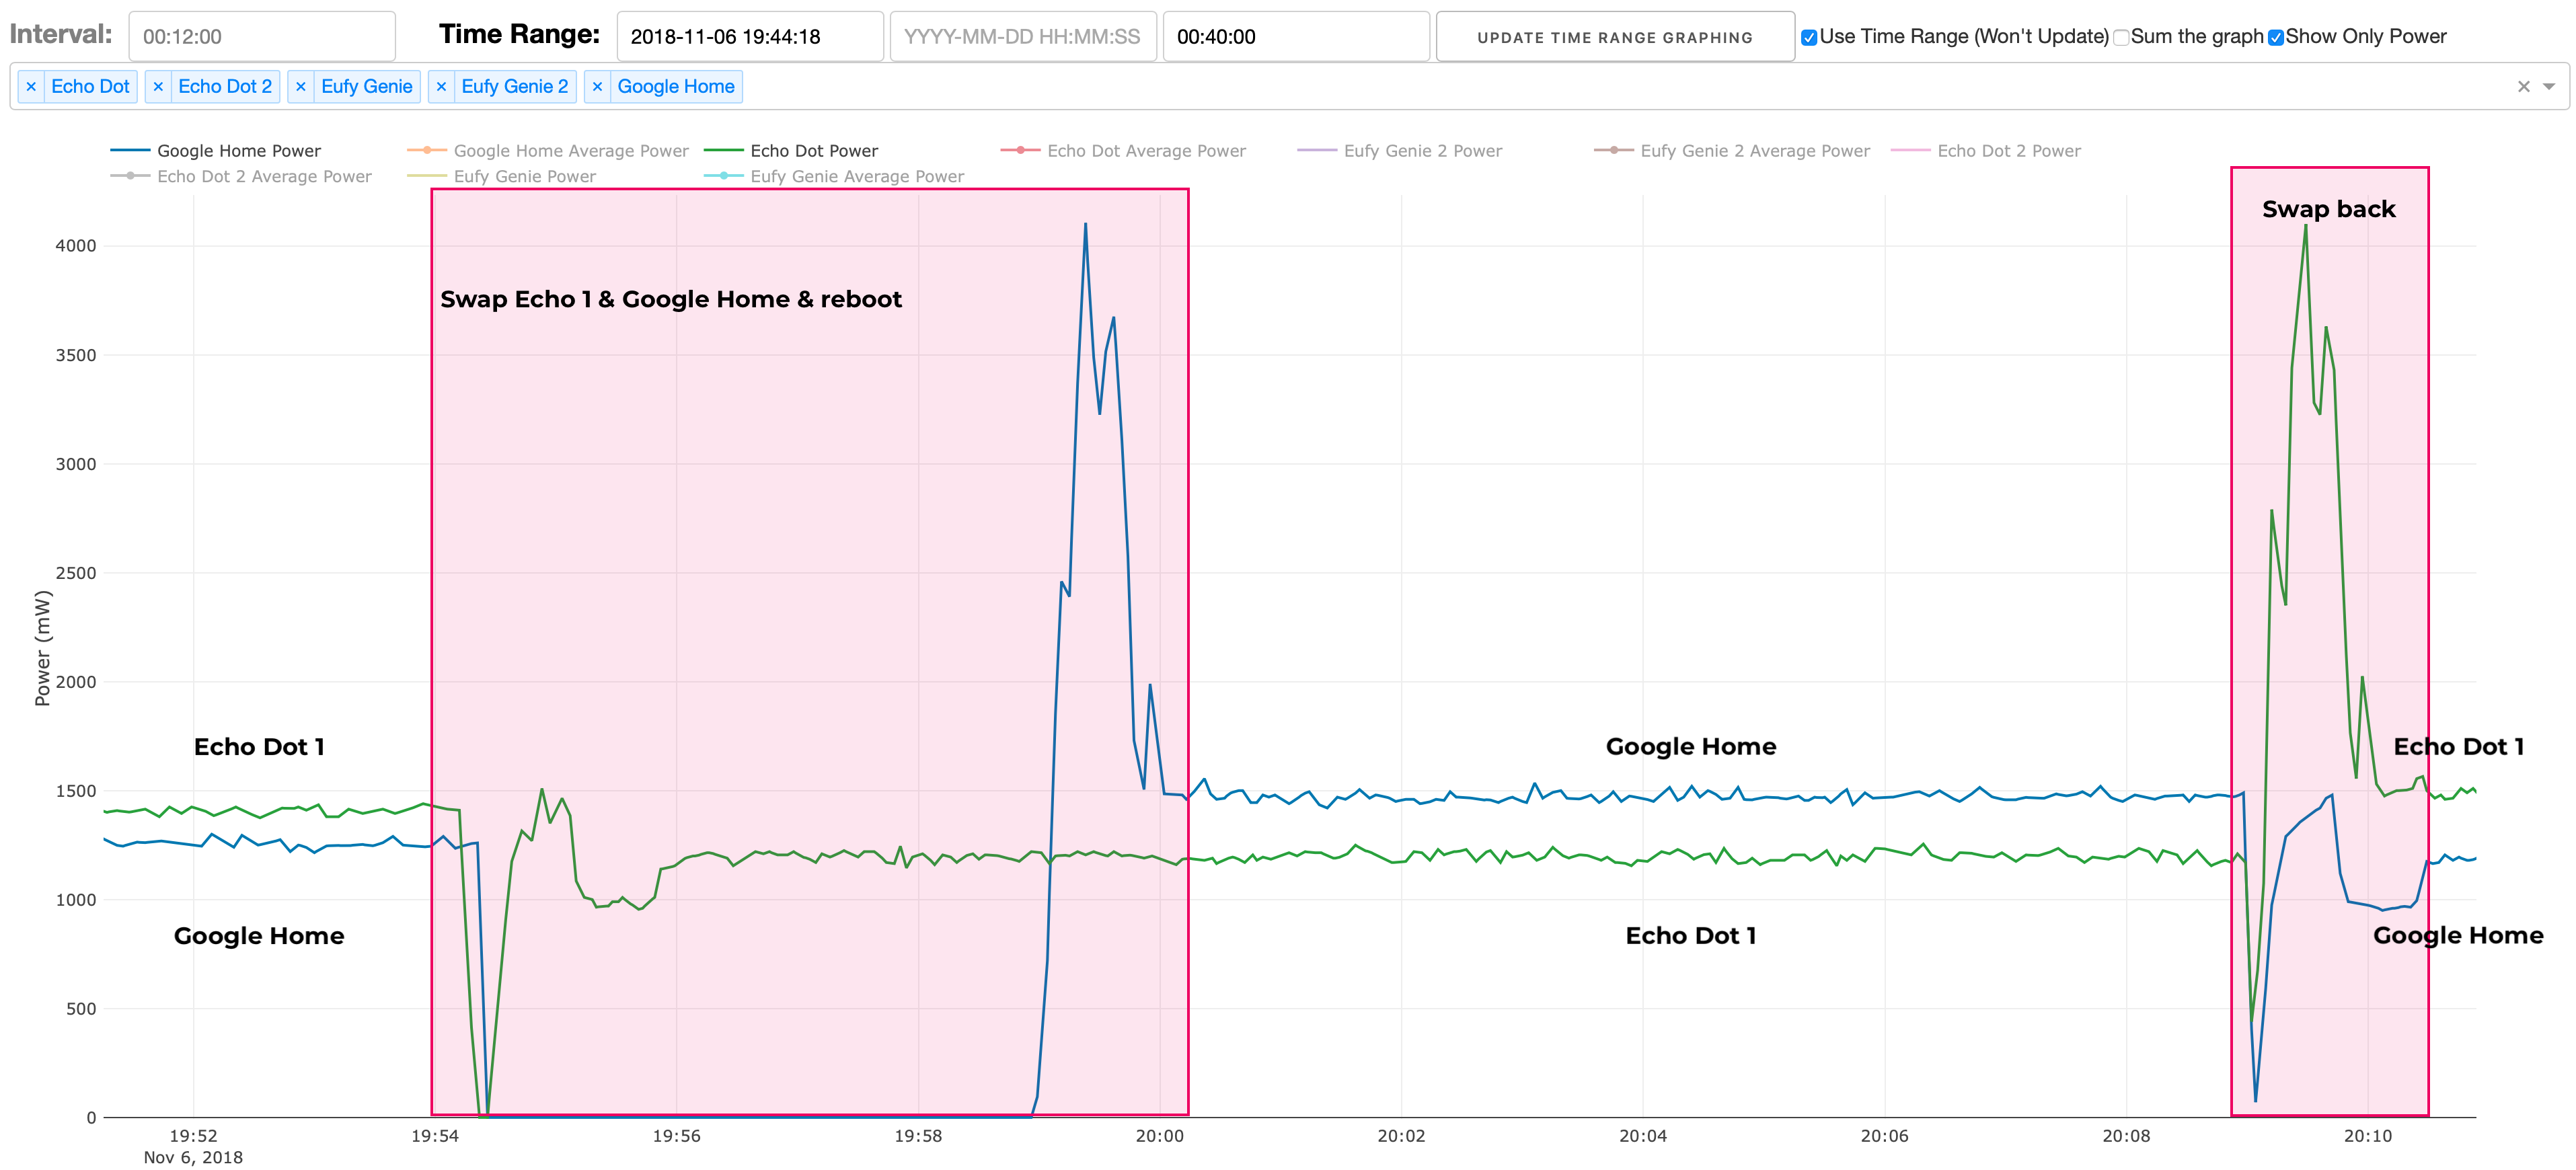
\includegraphics[width=1\textwidth]{figures/swapEcho1Home.png}
    \caption{Connected the Echo Dot 1 to WeMo for `Eufy Genie 1' and vice versa. The traces swap before and after switching.}
    \label{fig:swapEcho1Home}
\end{figure}

\begin{figure}[H]
    \centering
    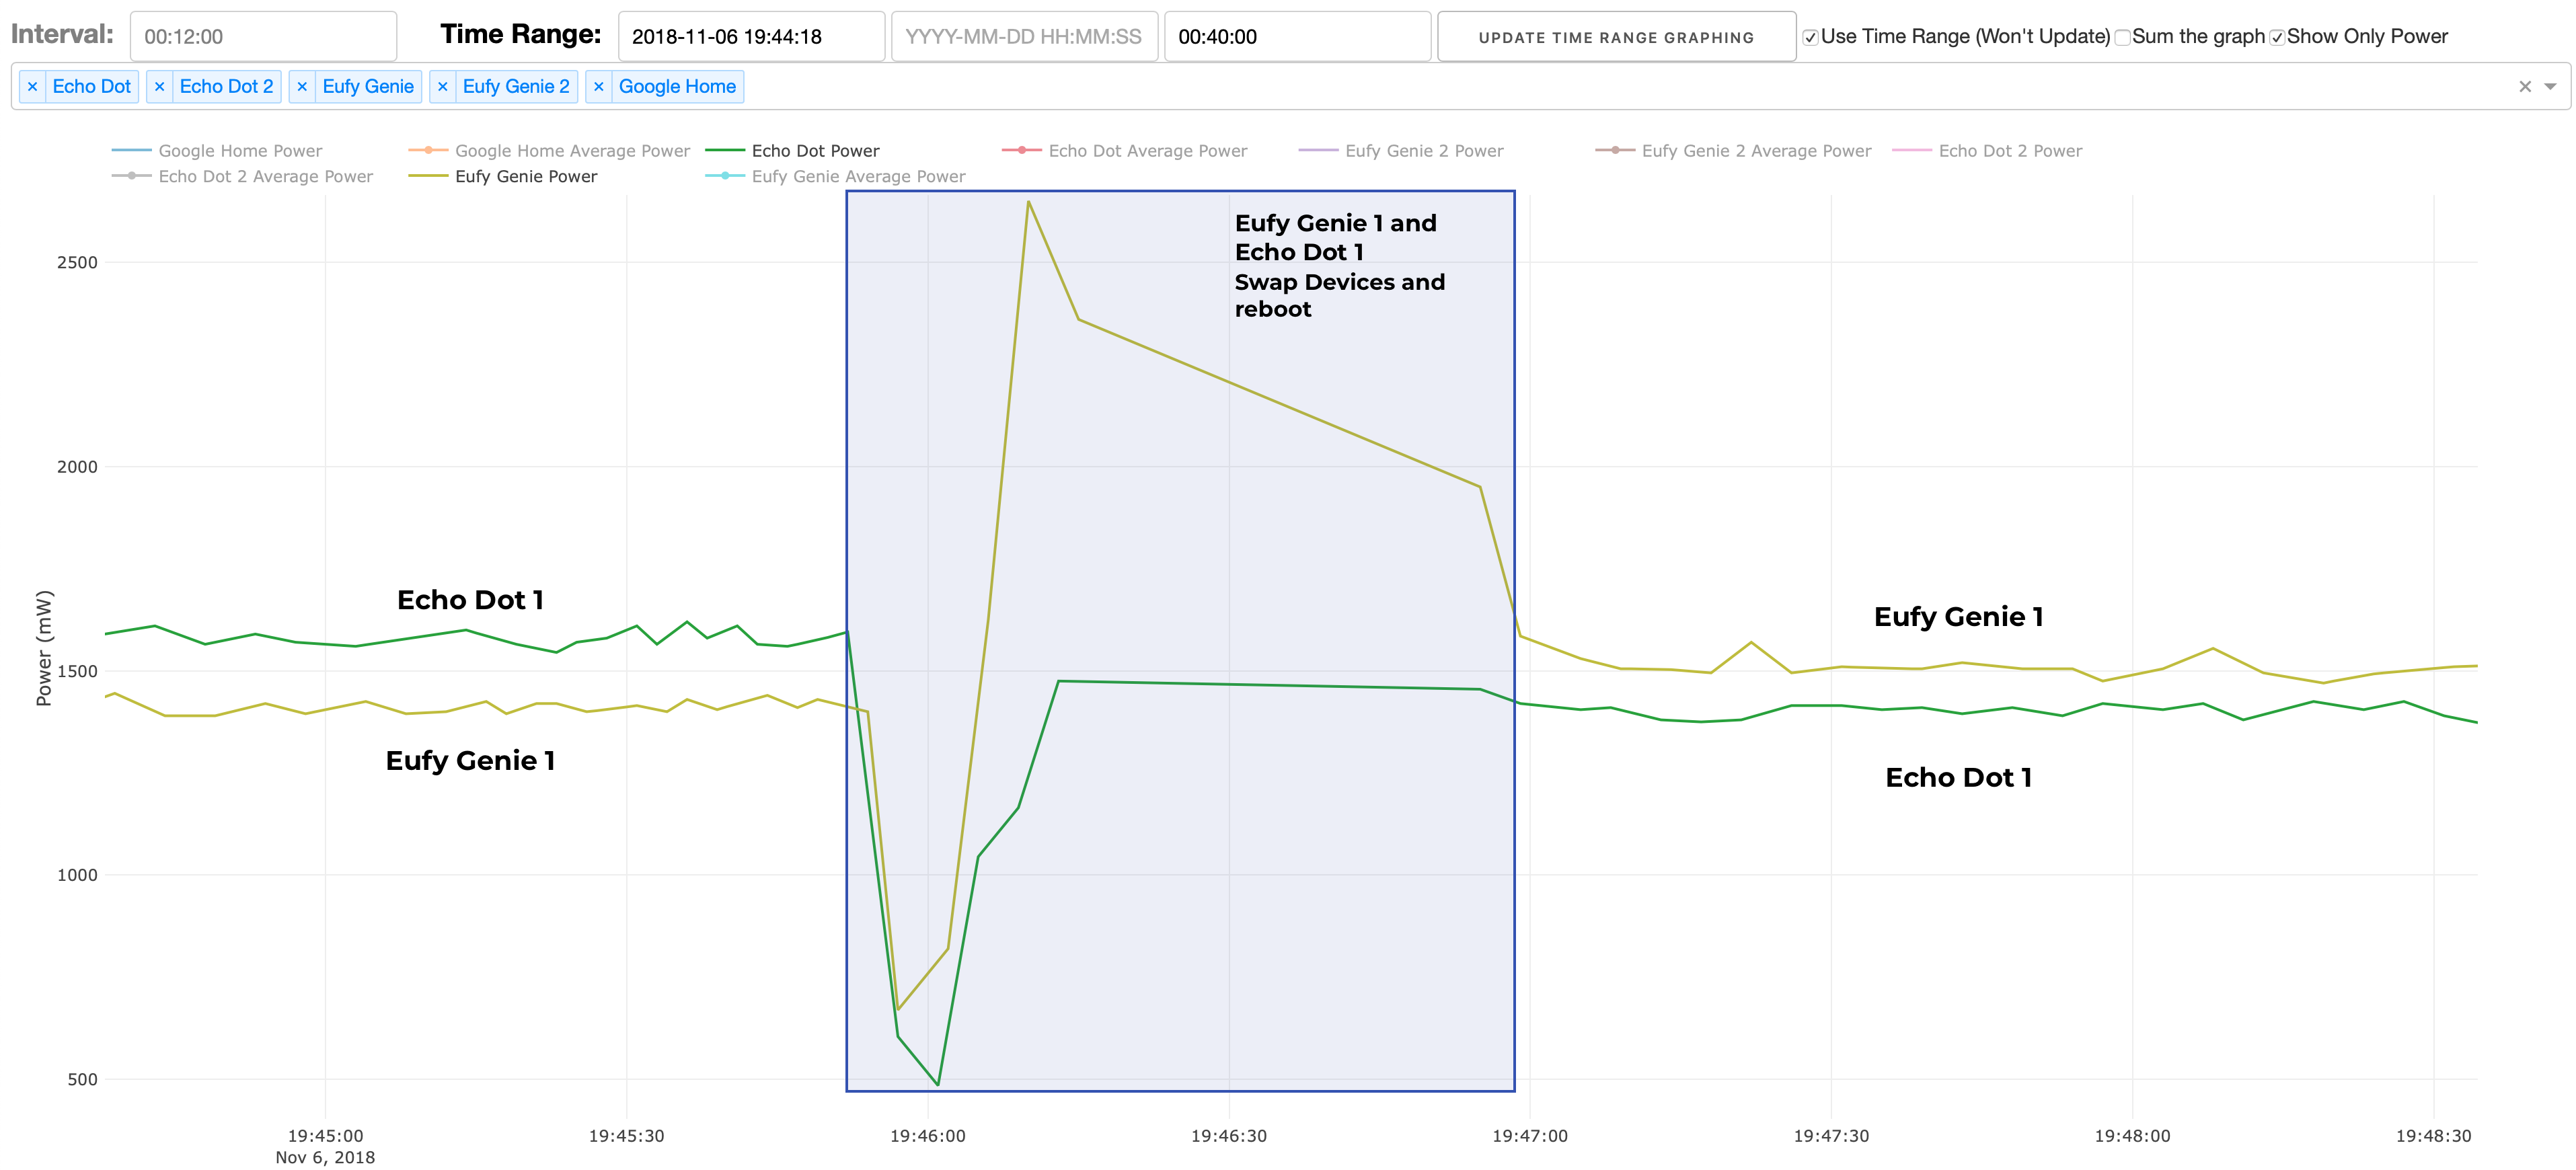
\includegraphics[width=1\textwidth]{figures/swapEufy1Echo1.png}
    \caption{Connected the Eufy Genie 1 to WeMo for `Echo Dot 1' and vice versa. The traces swap before and after switching.}
    \label{fig:swapEufy1Echo1}
\end{figure}

\begin{figure}[H]
    \centering
    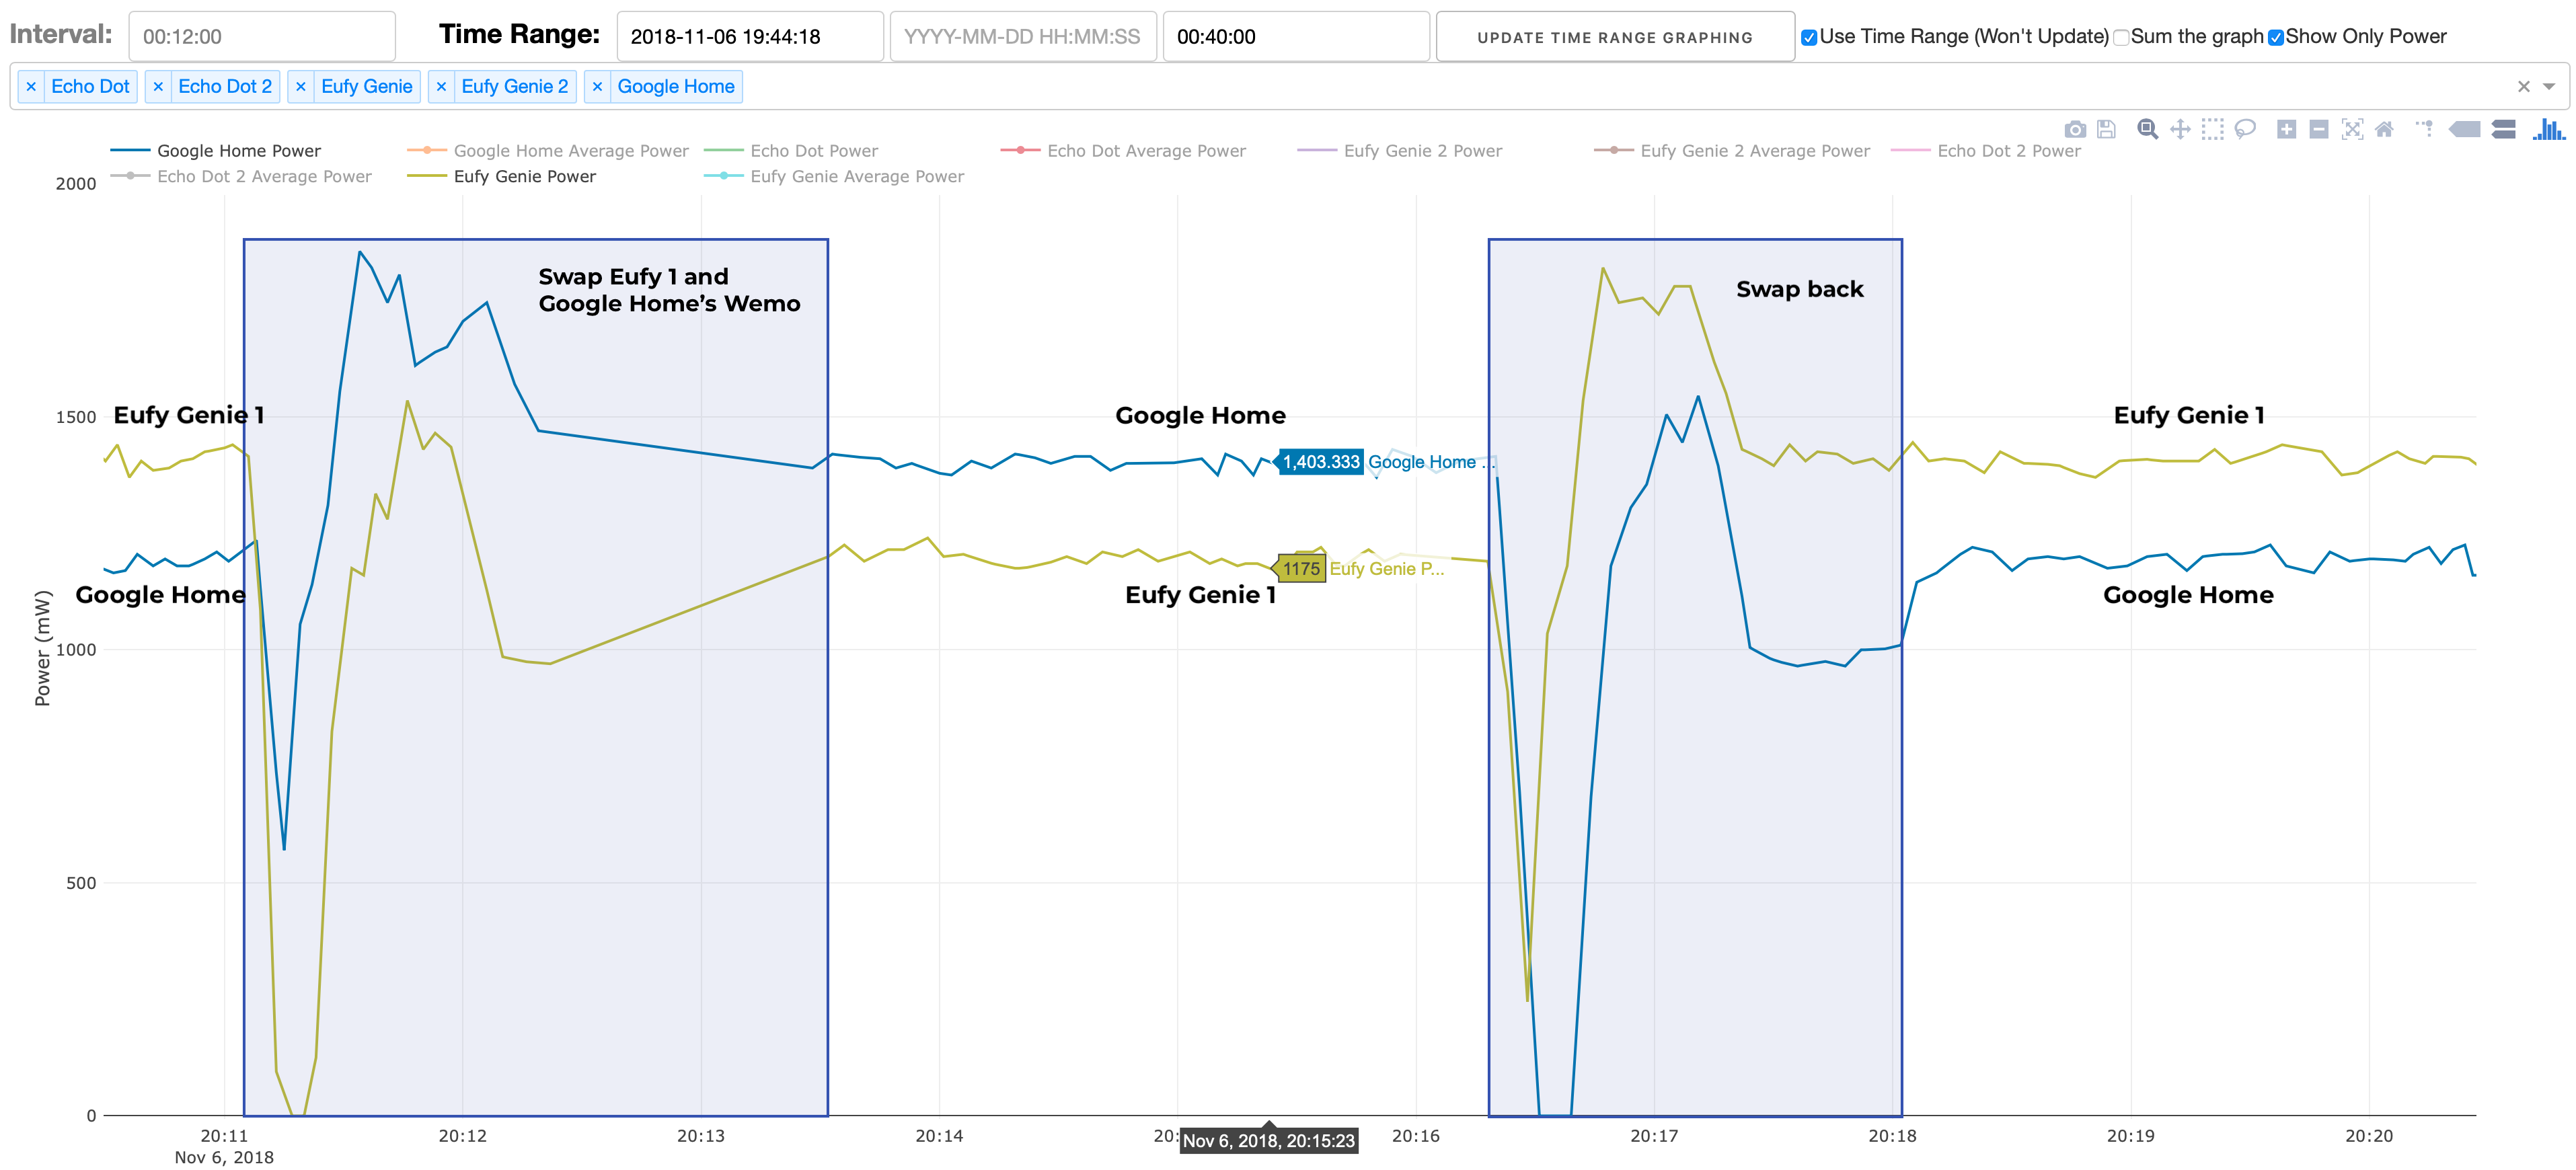
\includegraphics[width=1\textwidth]{figures/swapEufy1Home.png}
    \caption{Connected the Google Home to WeMo for `Eufy Genie 1' and vice versa. The traces swap before and after switching.}
    \label{fig:swapEufy1Home}
\end{figure}

\section{General Analysis}
\label{General Analysis}
The figures shown in this section give examples of how the database and grapher tool is used. The figures also demonstrate a strong correlation between what the device is doing and its network/power usage, serving as data to fingerprint each smart speaker.

Frawley's paper contains a more in-depth analysis of this topic. His paper includes GeoIP \cite{maxmind} information from Cal Poly's ITS servers \cite{its} that highlights the locations and companies the network packets are sent to and received from. Frawley's paper also includes data of unencrypted packets being sent and received along with the text within them.

\subsection{Google Home Mini General Analysis}
The Google Home Mini's idle traffic broadcasts SSDP (Simple Service Discovery Protocol) packets once every minute. The SSDP packets are a discovery request packet for every IoT device on the network that supports UPnP (Universal Plug and Play). After devices such as the Echo Dot, Samsung TV, and the Chromebook receive an SSDP packet, they respond with information about themselves in a .xml file. This XML file contains details regarding the device operating system and more. Google also sends encrypted TCP packets to Google every 10 minutes. Figure \ref{fig:home} shows the Google Home Mini's idle traffic. The large spikes are the encrypted TCP packets, and the smaller spikes are the SSDP/UPnP packets.

\begin{figure}[H]
  \centering
    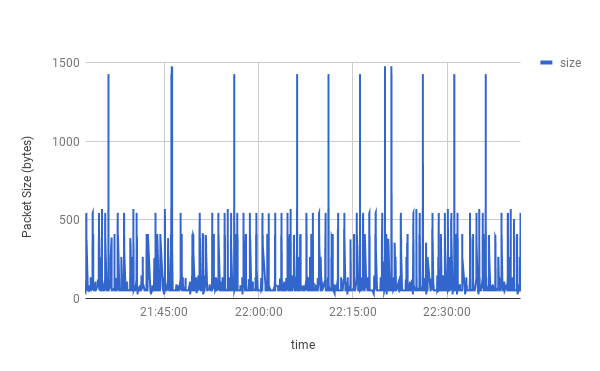
\includegraphics[width=0.9\textwidth]{home1hr}
  \caption{Idle Traffic of Google Home Over 1 Hour Period}
  \label{fig:home}
\end{figure}

Figure \ref{fig:homequery} shows a graph of the Google Home Mini's network and power usage while performing various commands. The Google Home Mini is first asked for the news and then told to stop. After waiting for 40 minutes, we ask it for the weather forecast.

\begin{figure}[H]
  \centering
    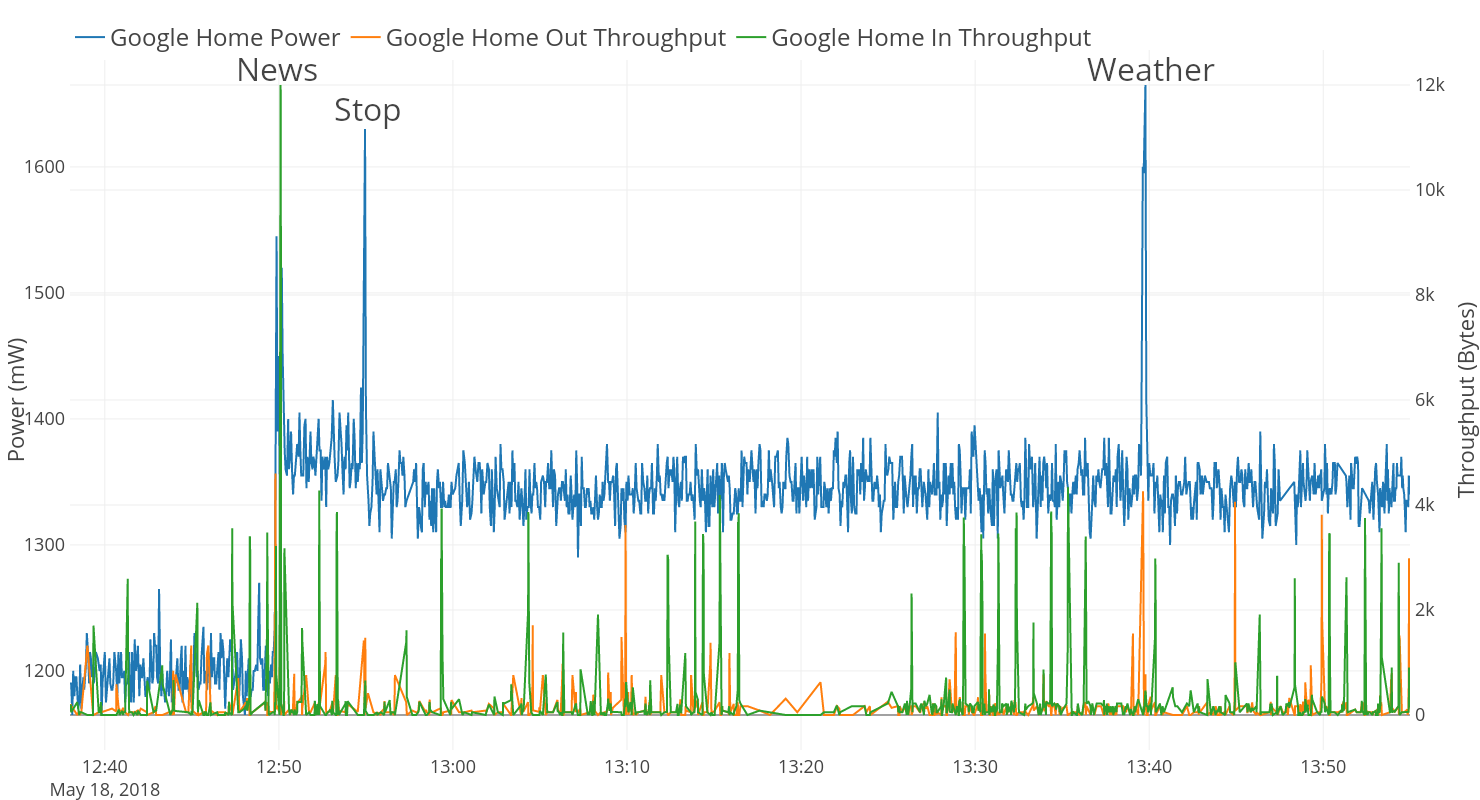
\includegraphics[width=1\textwidth]{homequery}
  \caption{Home Mini Response to News and Weather}
  \label{fig:homequery}
\end{figure}

\subsubsection{Google Chromecast}
Figure \ref{fig:ccboth} shows the Chromecast initial startup graph. On startup, the Chromecast shows an intro tutorial video and downloads a firmware update. After rebooting twice, it is ready to go.

\begin{figure}[H]
  \centering
  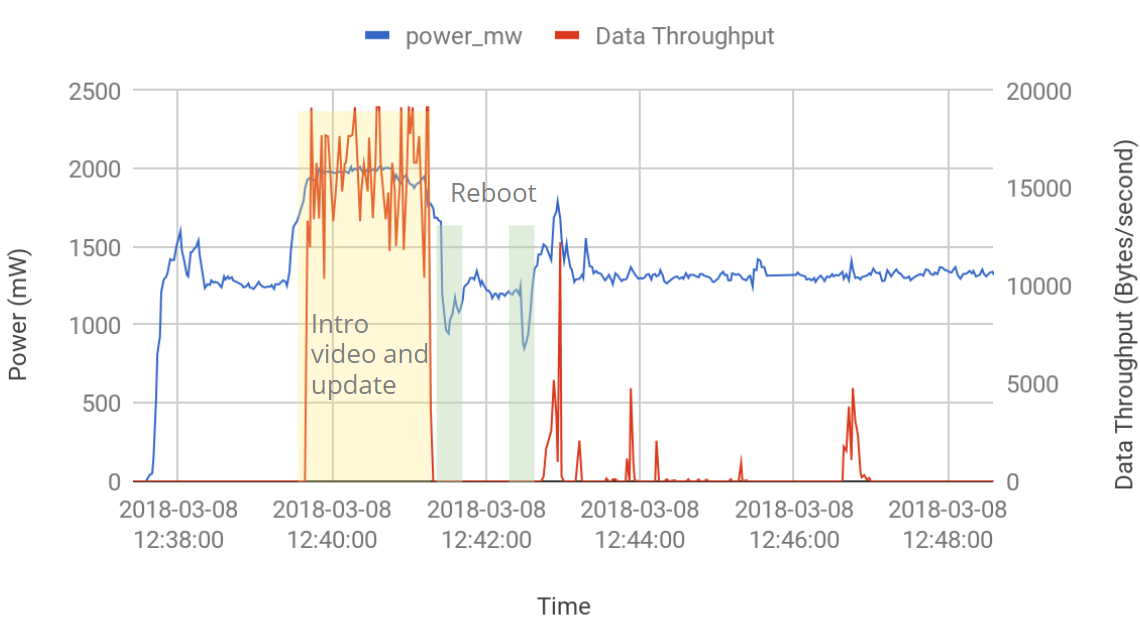
\includegraphics[width=1\textwidth]{ccboth}
  \caption{Chromecast First Time Boot Network Traffic and Power Consumption}
  \label{fig:ccboth}
\end{figure}

Figure \ref{fig:ccstream} shows the Chromecast streaming graph. In this time frame, the Chromecast streams video in the marked box.

\begin{figure}[H]
  \centering
  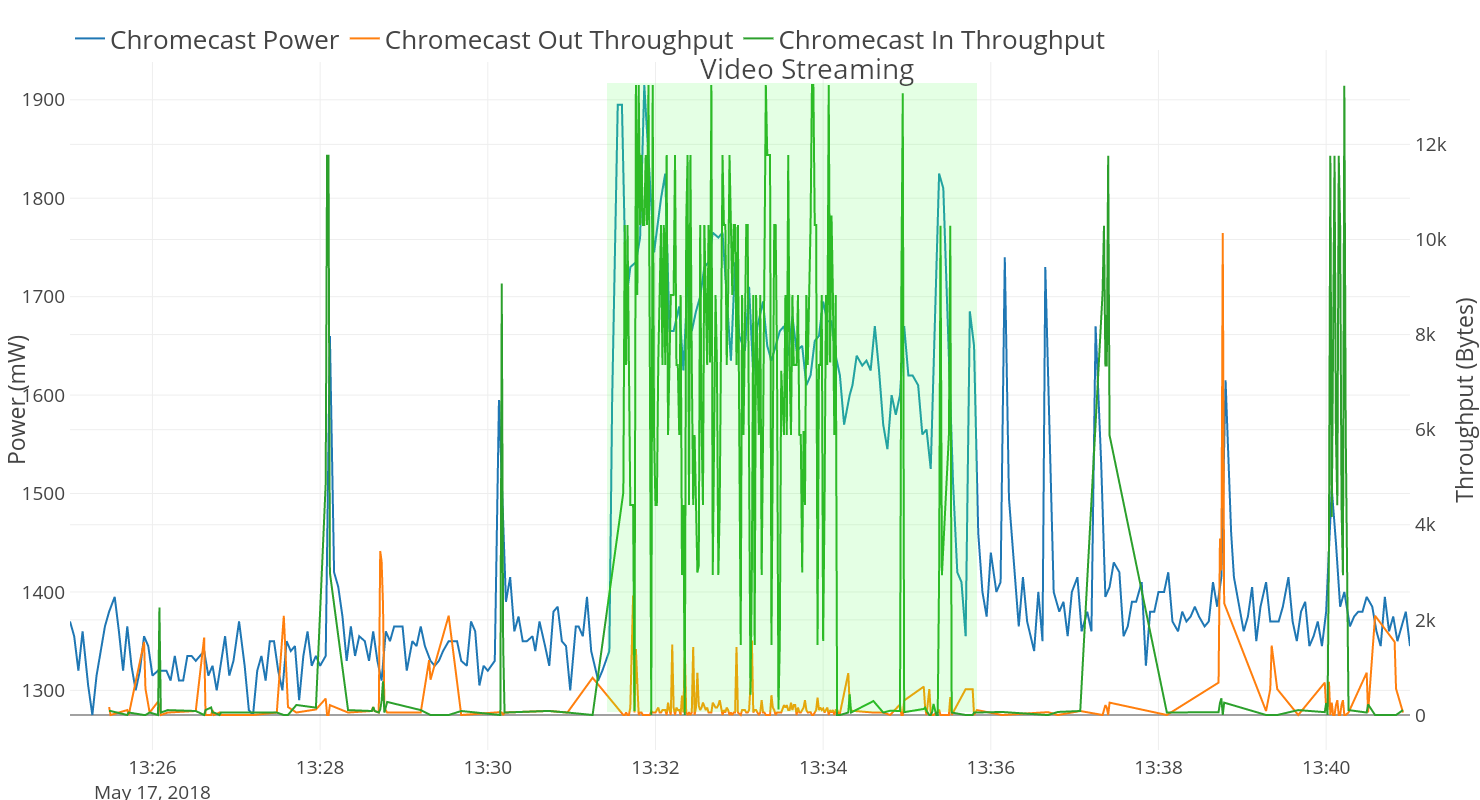
\includegraphics[width=1\textwidth]{ccstreaming}
  \caption{Chromecast Video Streaming}
  \label{fig:ccstream}
\end{figure}

Additionally, the Chromecast idle graph is shown in Figure \ref{fig:ccbg}. In this time frame, there are consistent spikes to the Chromecast every 2 minutes. During these spikes, the Chromecast is showing a new background that it downloads from Google Servers.

\begin{figure}[H]
  \centering
  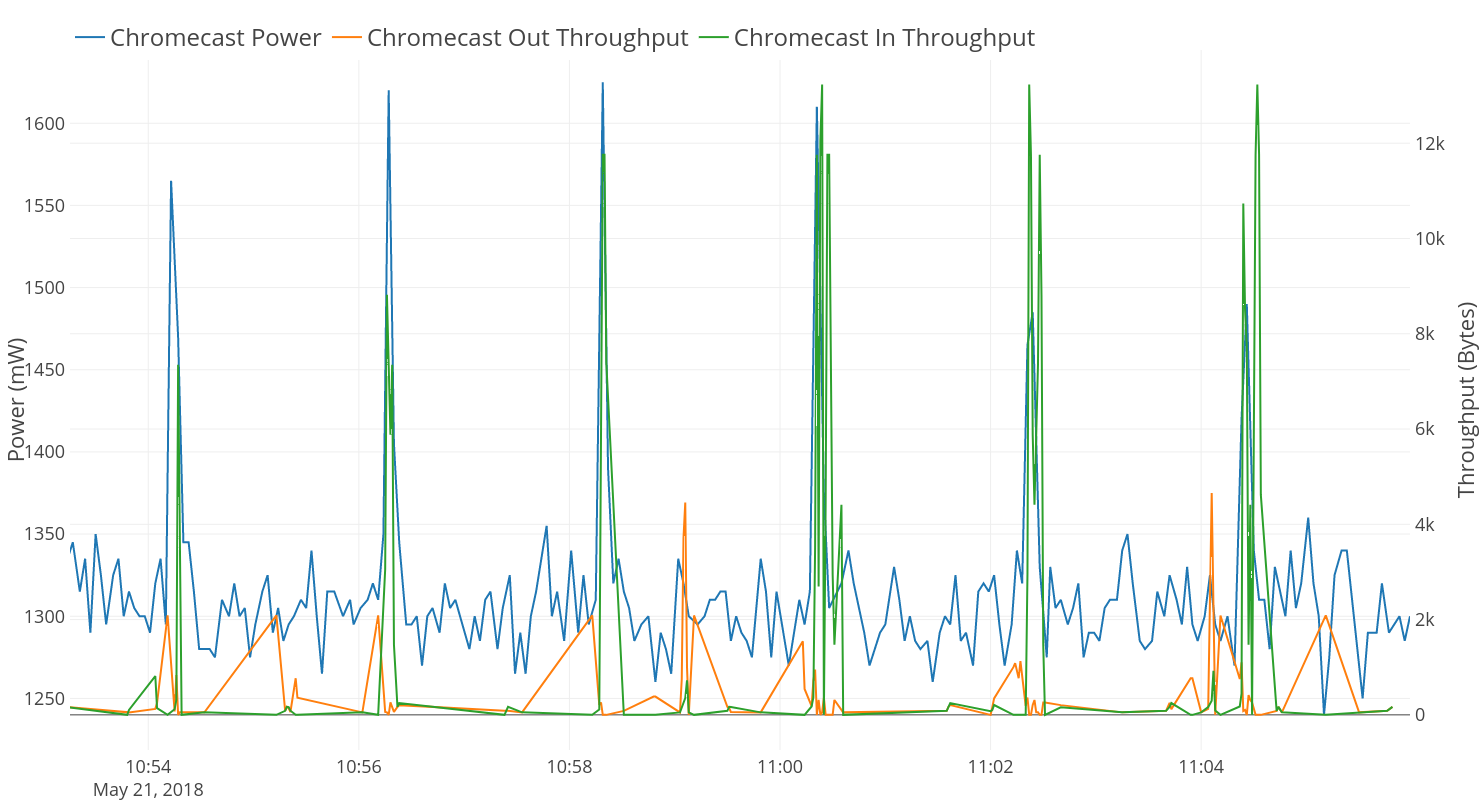
\includegraphics[width=1\textwidth]{chromecastbg.png}
  \caption{Chromecast Idle Traffic}
  \label{fig:ccbg}
\end{figure}

\subsubsection{Amazon Fire Stick}

\begin{figure}[H]
  \centering
  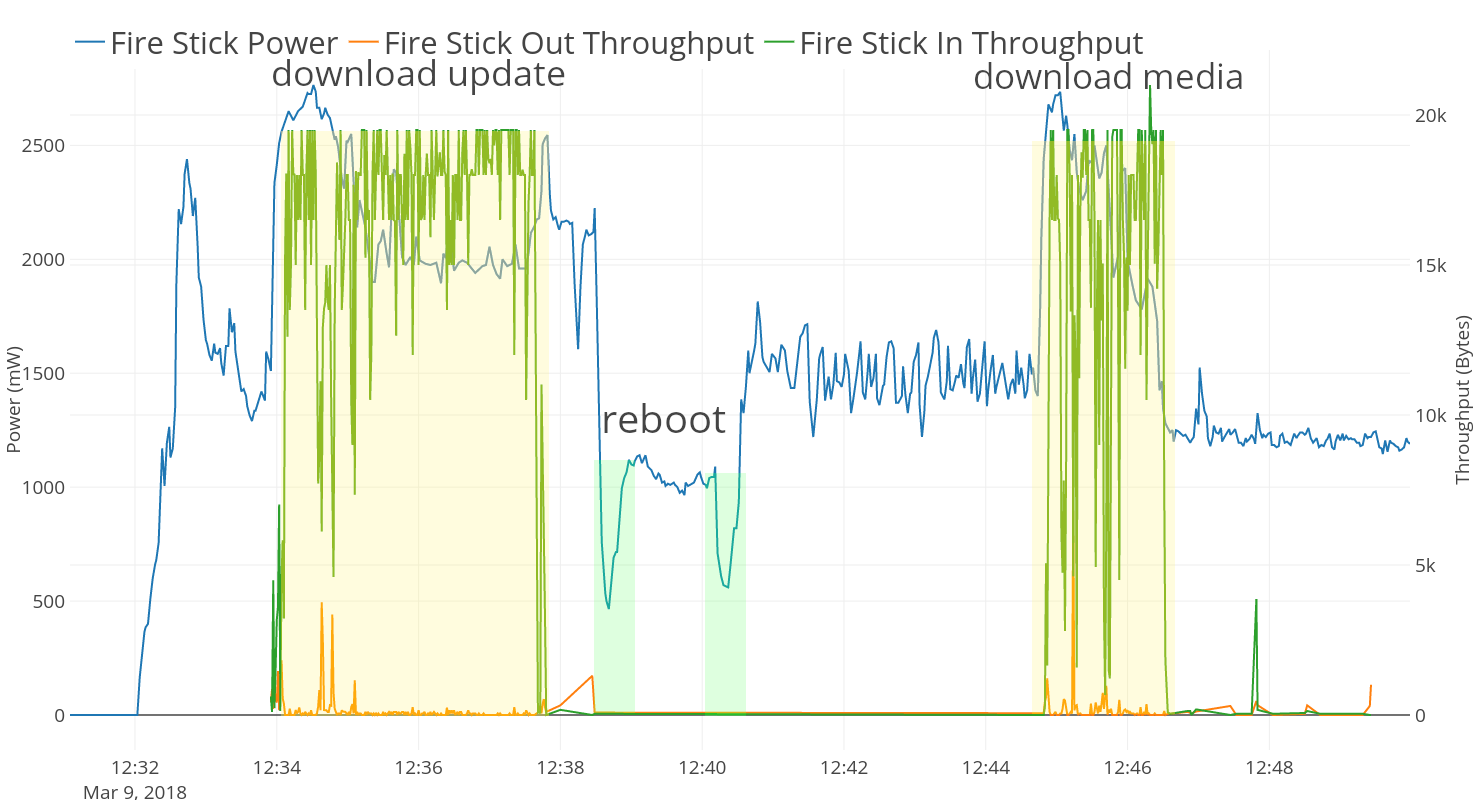
\includegraphics[width=1\textwidth]{fireboot}
  \caption{Fire TV Stick First Time Boot Network Traffic and Power Consumption}
  \label{fig:fireboth}
\end{figure}

Figure \ref{fig:fireboth} shows the Amazon Fire Stick startup graph. On first boot, the fire stick downloads an update, reboots twice, then downloads certificates from Symantec and Verisign.

When streaming, the Fire Stick increases throughput and power usage with a spike at the beginning and end of streaming in power usage as shown in Figure \ref{fig:fsyt}.

\begin{figure}[H]
  \centering
  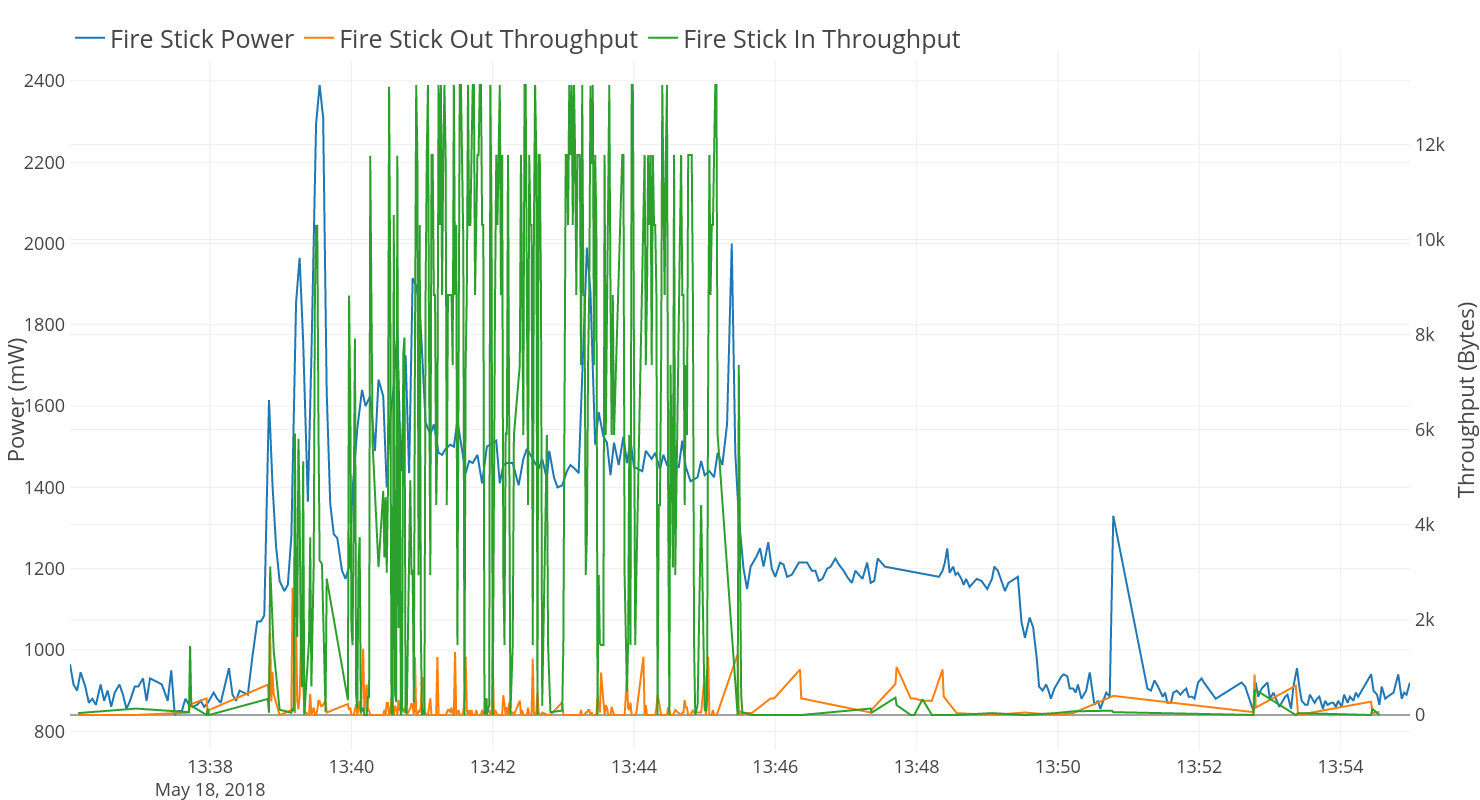
\includegraphics[width=1\textwidth]{fsyt}
  \caption{Fire TV Stick Video Streaming}
  \label{fig:fsyt}
\end{figure}

\subsubsection{Roku Express}
When streaming, the Roku's power usage and network throughput rise and stay at a constant level until the video streaming is complete. At which point it drops back down when done.

\begin{figure}[H]
  \centering
  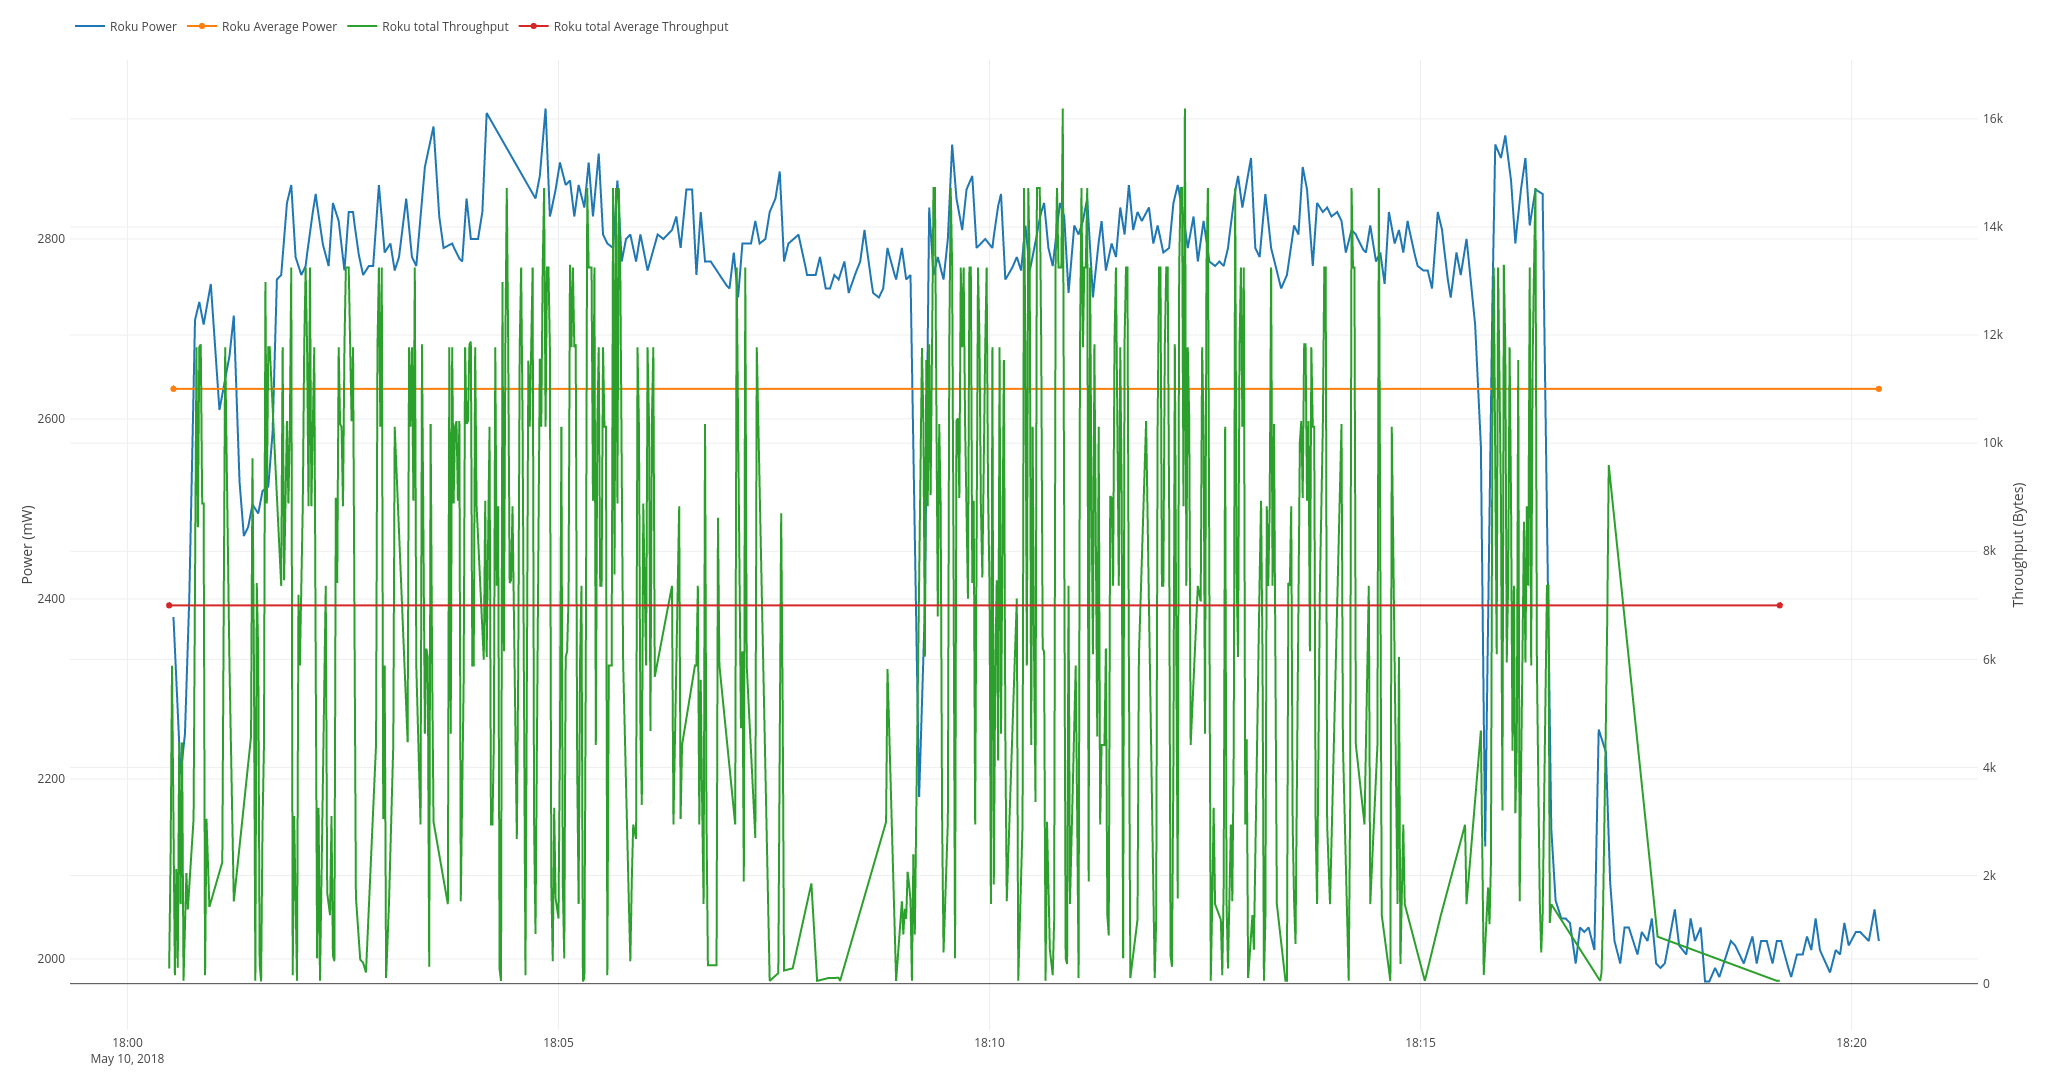
\includegraphics[width=1\textwidth]{figures/rokuStreaming.png}
  \caption{Roku Express Video Streaming}
  \label{fig:rokuStreaming}
\end{figure}

\subsection{General Analysis Discussion}
From all the figures in this section, there is a visual correlation between network/power usage and what each device is doing. During periodic updates, the smart speakers and streaming devices have periodic network/power usage spikes as shown in Figure \ref{fig:ccbg}. While streaming, the power/network usage increases for the period of the stream as shown in \ref{fig:ccstream}, \ref{fig:fsyt}, and \ref{fig:rokuStreaming}. This strong correlation shows the value of the database and visualizer tool for IoT device analysis. It also indicates that it may be possible to use network throughput/power usage over time to understand what a device is doing.

\section{Power Analysis on Smart Speakers}
\label{Power Analysis on Smart Speakers}
There is already significant analysis on network usage of IoT devices as shown in the previous works Section \ref{Previous Work}. This paper focuses on the smart speakers' power usage to focus the scope of research.

This section first examines the power usage of the smart speakers separately before examining total power usage in Section \ref{sumPowerGraph}.

\subsection{Smart Speaker Comparison}
\label{smartSpeakerComparisonSection}
This Subsection compares the energy and network usages of the three smart speakers individually and speculates trade-offs that they make.

In the Figures \ref{fig:smartSpeakerSeperate} and \ref{fig:smartSpeakerNetworkSeperate}, we display the power and network traces for the Echo Dot 1, Eufy Genie 1, and Google Home. We used the same time frame as the graph in Figure \ref{fig:bestBballSeperate} for the two graphs for Figures \ref{fig:smartSpeakerSeperate} and \ref{fig:smartSpeakerNetworkSeperate}. We removed the second Echo Dot 2 and Eufy Genie 2 so that there is one of each device.

In the time frame of Figures \ref{fig:smartSpeakerSeperate} and \ref{fig:smartSpeakerNetworkSeperate}, the average power, from greatest to least, starts with the Echo Dot (1650 mW), then the Eufy Genie (1325 mW), and the Google Home (1175 mW). For average throughput, from greatest to least, there is the Eufy Genie (1743 bytes), Google Home (800 bytes), and Echo Dot (325 bytes). These results are shown in Figure \ref{fig:smartSpeakerComparison}

\begin{figure}[H]
  \centering
  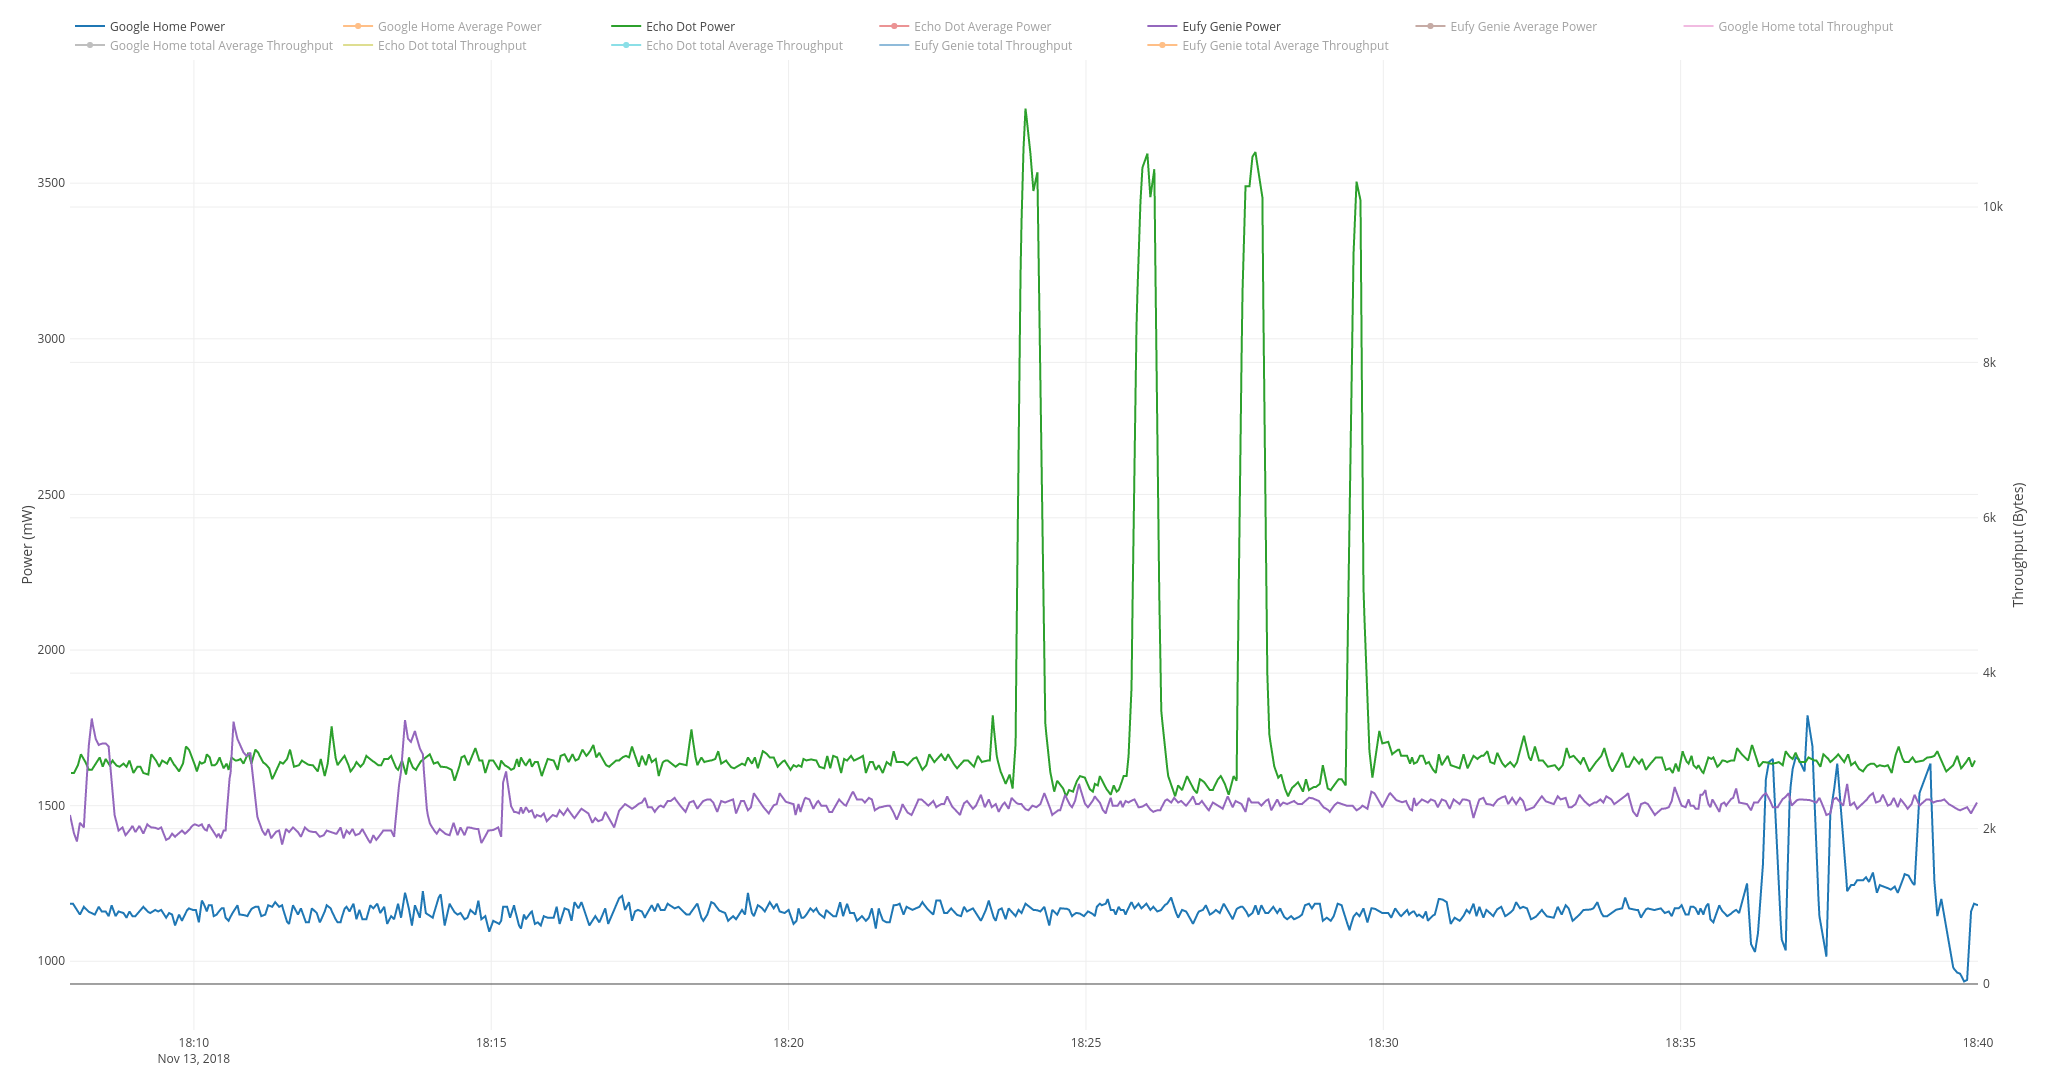
\includegraphics[width=1\textwidth]{figures/smartSpeakerSeperate.png}
  \caption{Power usage of Echo Dot 1, Eufy Genie 1, and Google Home over time when asked ``who is the best basketball player''. Same graph as Figure \ref{fig:bestBballSeperate} with Echo Dot 2 and Eufy Genie removed.}
  \label{fig:smartSpeakerSeperate}
\end{figure}

\begin{figure}[H]
  \centering
  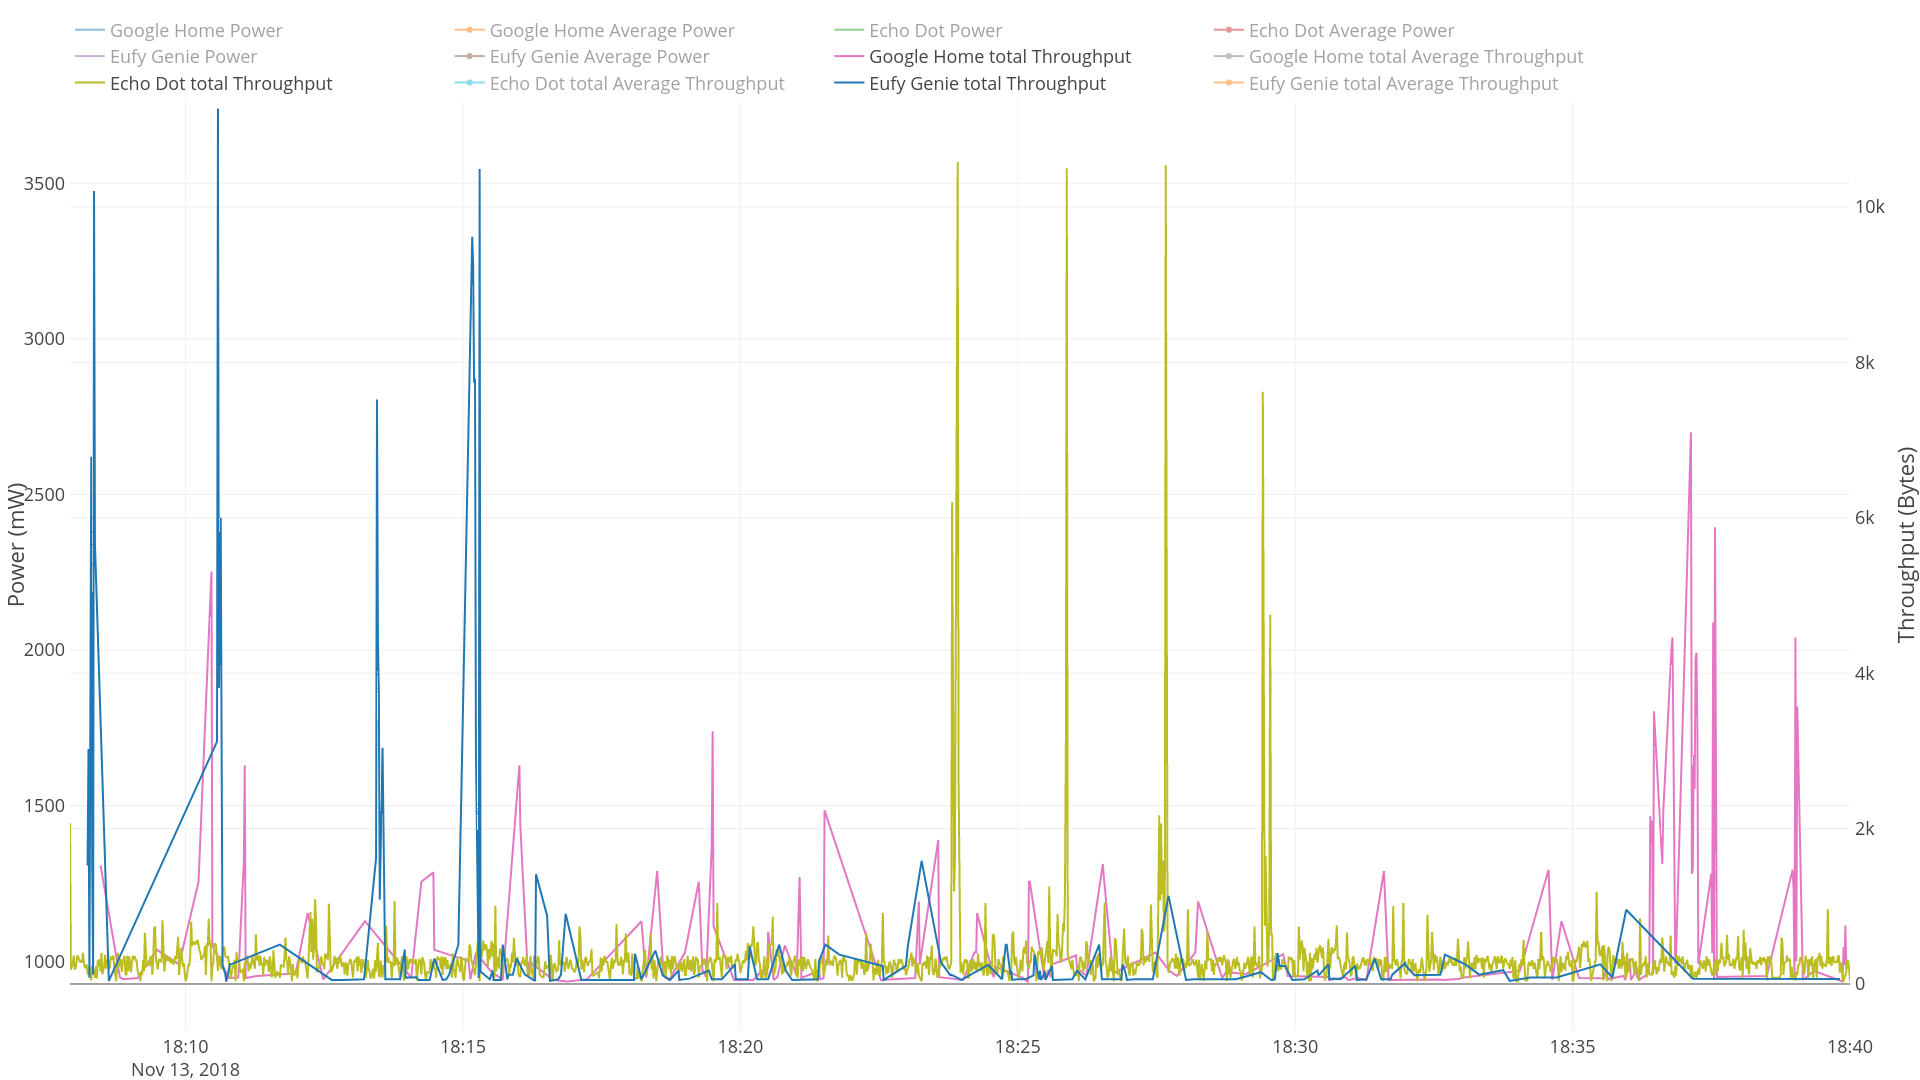
\includegraphics[width=1\textwidth]{figures/smartSpeakerNetworkSeperate.png}
  \caption{Power usage of Echo Dot 1, Eufy Genie 1, and Google Home over time when asked ``who is the best basketball player''. Same time frame as Figure \ref{fig:smartSpeakerSeperate}}
  \label{fig:smartSpeakerNetworkSeperate}
\end{figure}

\begin{figure}[H]
    \centering
    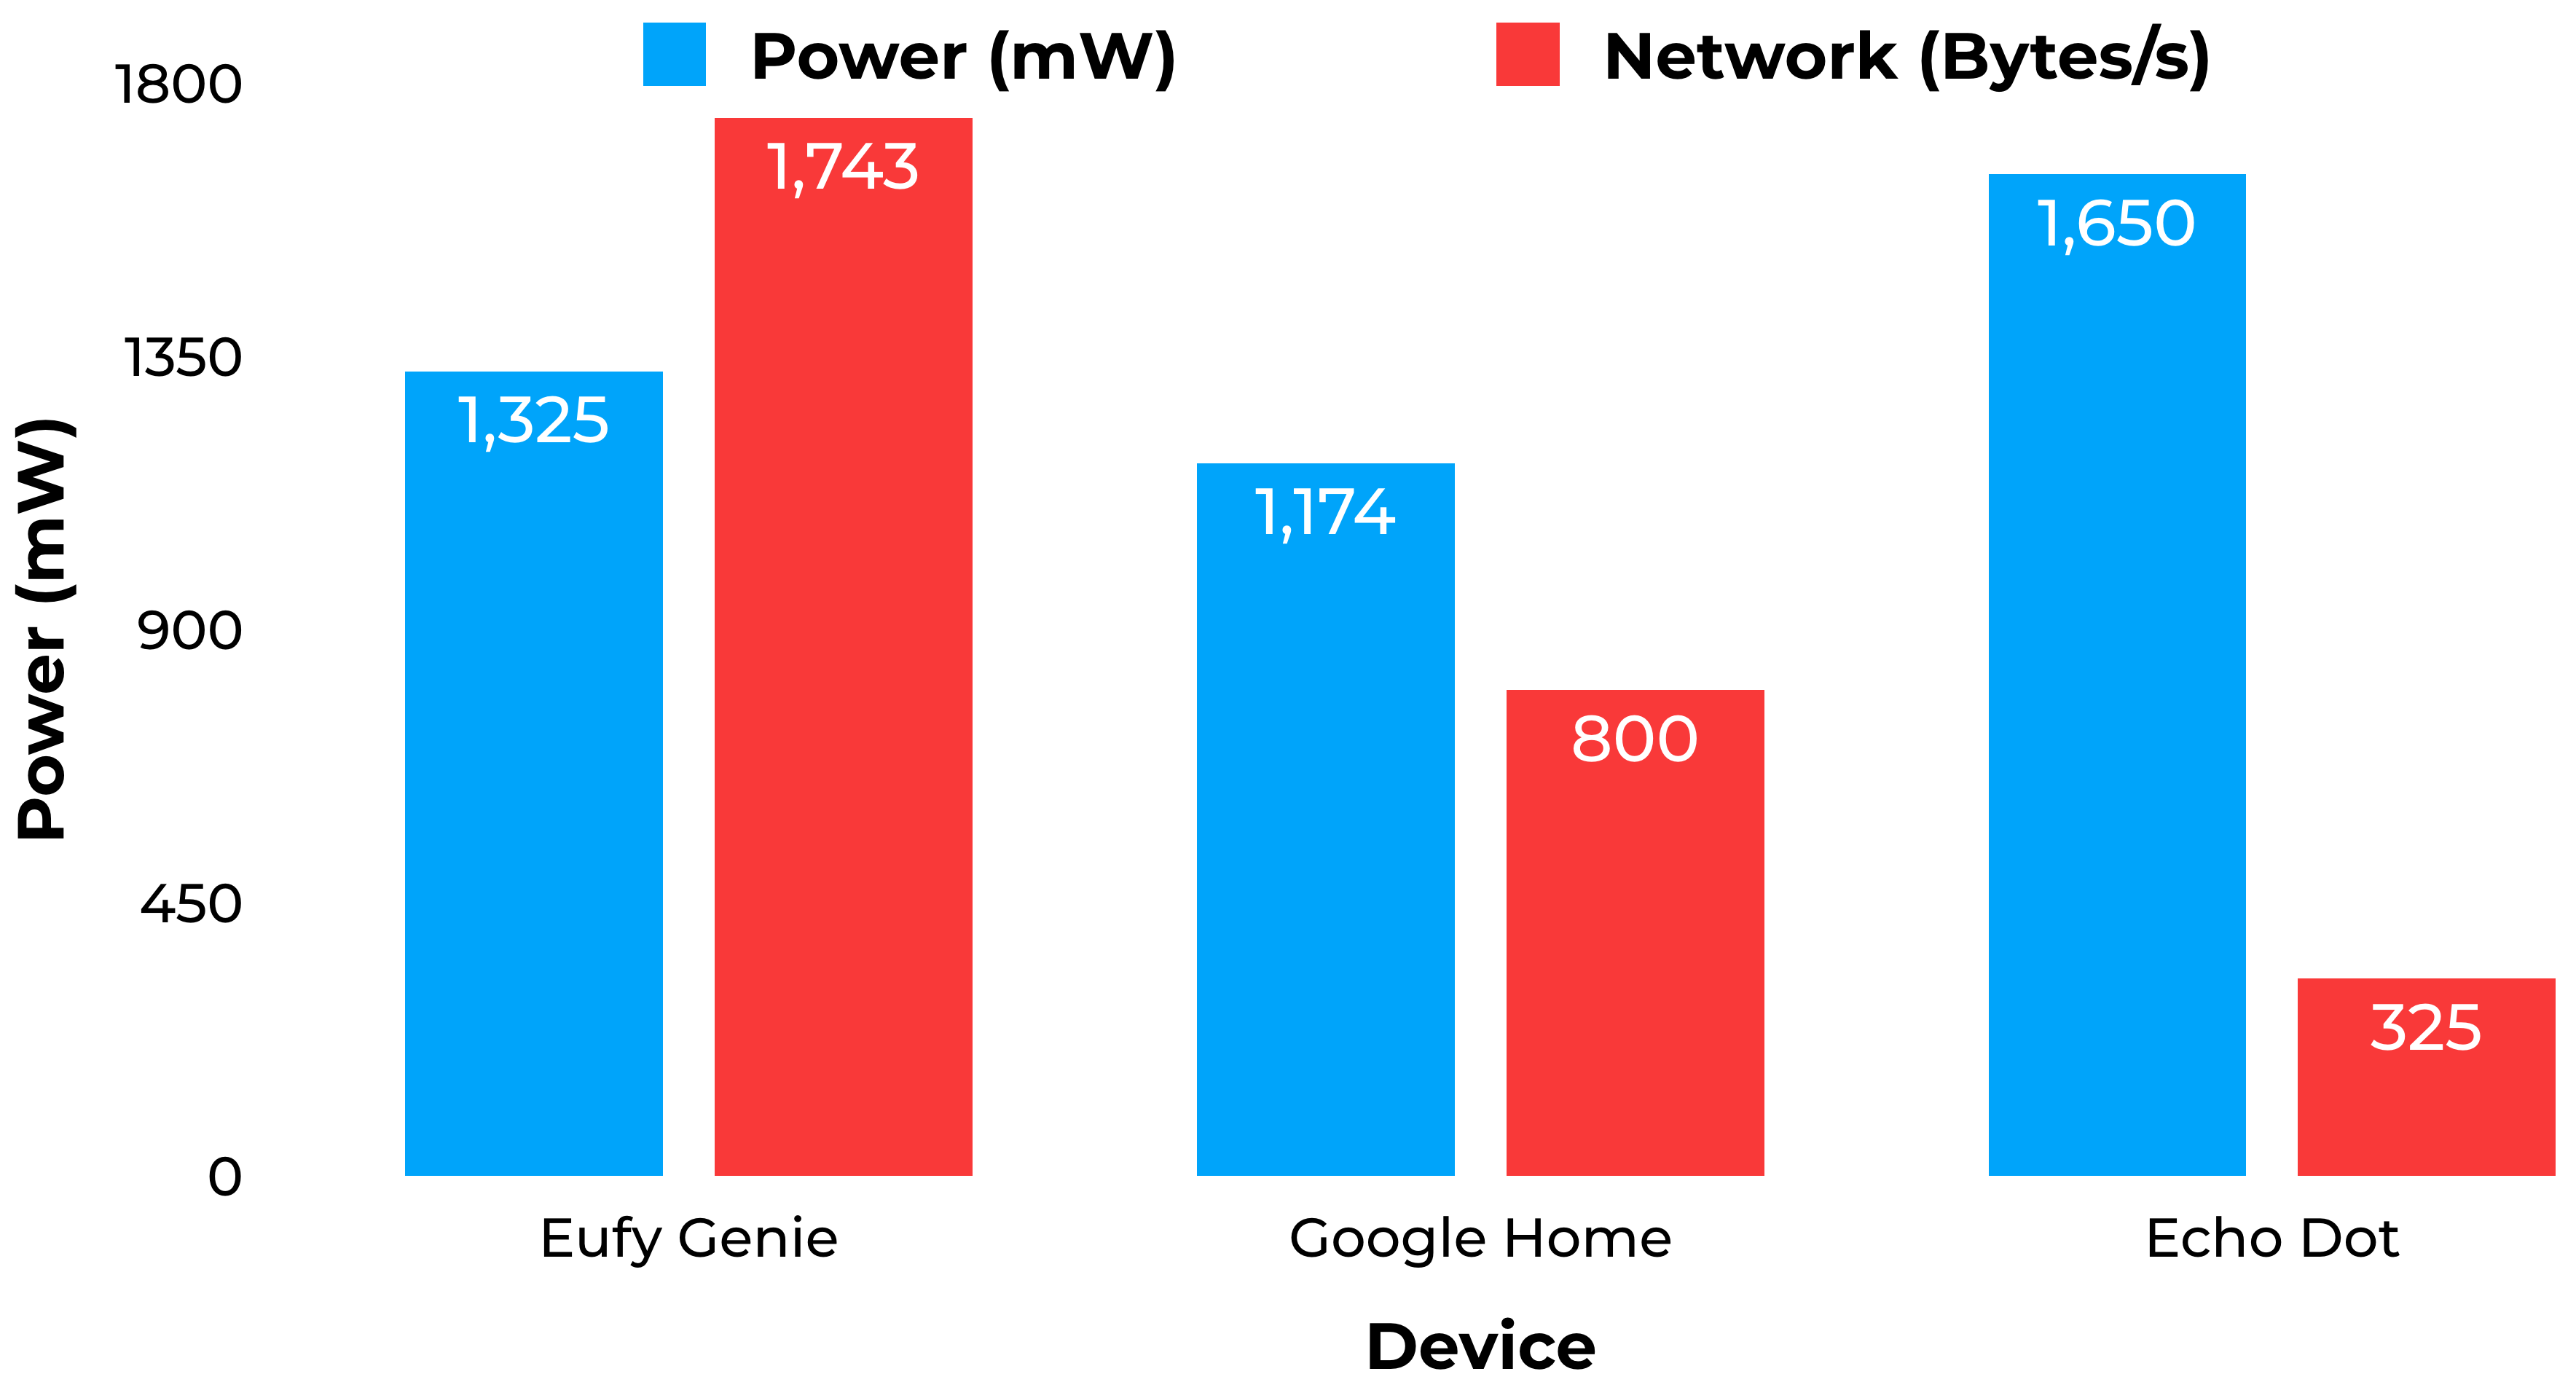
\includegraphics[width=1\textwidth]{figures/smartSpeakerComparison.png}
    \caption{Average power and network usage at each second for the Echo Dot, Eufy Genie, and Google Home in the time frame of Figures \ref{fig:smartSpeakerSeperate} and \ref{fig:smartSpeakerNetworkSeperate}}
    \label{fig:smartSpeakerComparison}
  \end{figure}

From Figure \ref{fig:smartSpeakerComparison}, we can see that the Echo uses the most power, then the Eufy, then the Google Home. However, the Eufy uses the most network throughput, then the Google Home, then the Echo Dot. At its core, we believe each device is making some tradeoff between power and network usage. Possibly, the Echo dot is trying to do as much on board operations as possible, increasing the power usage. Possibly, the Eufy Genie is constantly querying for information, thus reducing power usage, but increasing network usage. Possibly, the Echo Dot has poor power optimizations. Further analysis to see why could be interesting.

\subsection{Echo Dot Brightness Sensor}
\label{Echo Dot Brightness Sensor}
One interesting finding from the Echo Dot is that it has a light sensor When turning on the room lights, the LEDs on the Echo Dot brighten to adapt. The brightness change causes the Echo Dot to use more idle power as shown in Figure \ref{fig:echolights}.

Figure \ref{fig:echolights} shows that the power usage of an Echo Dot can show if the lights are on in a house. This can help someone determine if someone is in their house or not or what room they are in, potentially introducing some privacy concerns.

\begin{figure}[H]
    \centering
    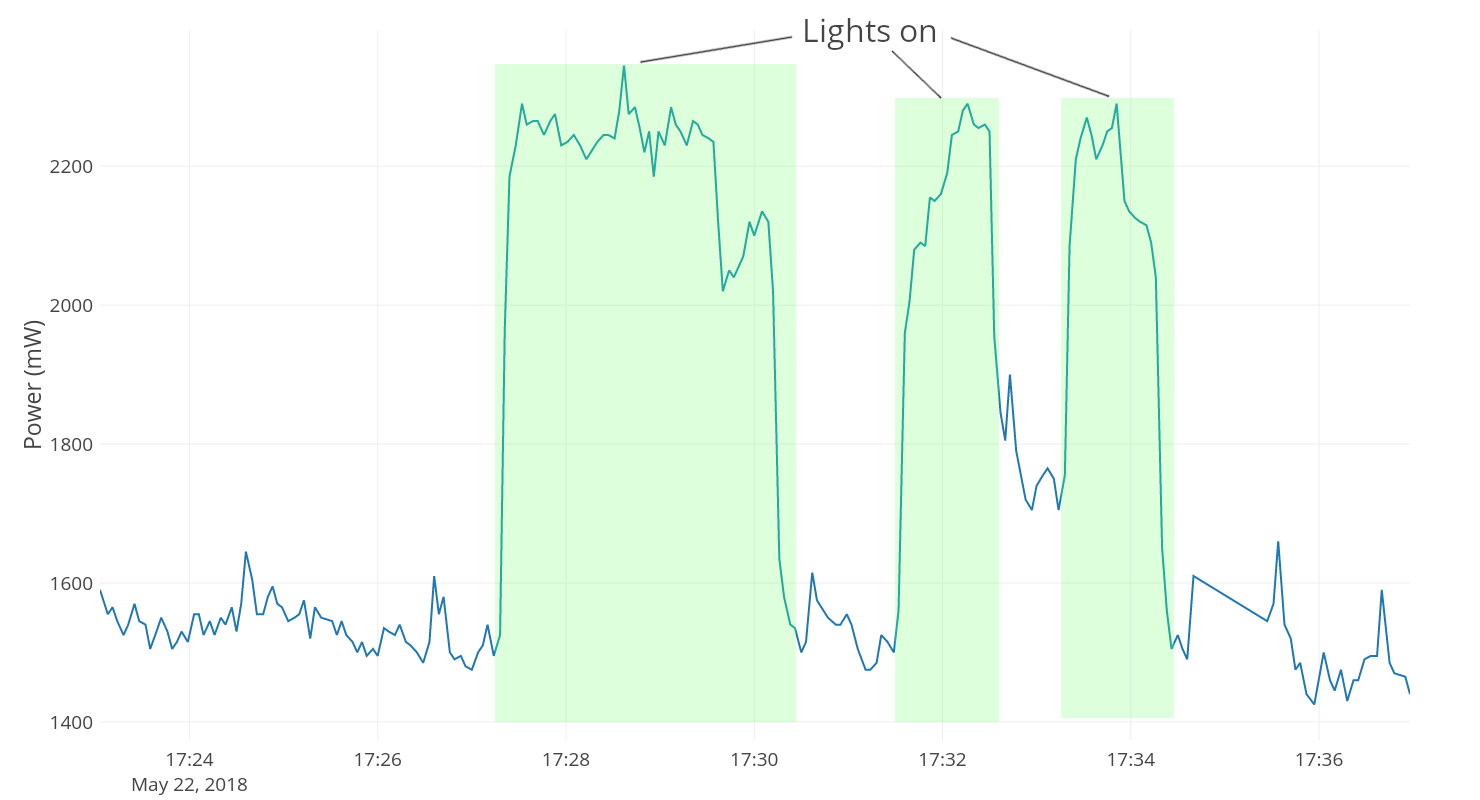
\includegraphics[width=1\textwidth]{echolights}
    \caption{Echo Dot Response to Lights}
    \label{fig:echolights}
\end{figure}

\subsection{Baseline Speaker Power}
\label{Baseline Speaker Power}
To determine what else can be learned from a smart speaker's power usage, this section examines the idle power of each smart speaker. Figure \ref{fig:baselineSpeakerPower} shows this from 1:00 AM to 2:30 AM when none of the devices are in use.

The Echo Dot 1 has the highest idle power as shown in the pink trace, the Echo Dot 2 has second highest idle power as shown in the green trace, the Eufy 1 and Eufy 2 have roughly the same idle power usage as shown in the yellow and purple traces, and the Google Home has the lowest idle power usage as shown in the blue trace. With visual analysis, the smart speaker can be matched to idle power usage. But the power usages can overlap between the Echo Dot 2 and Eufys. This makes it difficult to differentiate them and shows this method to identify a device is difficult. Also, on a shared powerline where the all power use is combined, these idle traces disappear, with no way to differentiate what idle devices are contributing to the total power usage.

\begin{figure}[H]
    \centering
    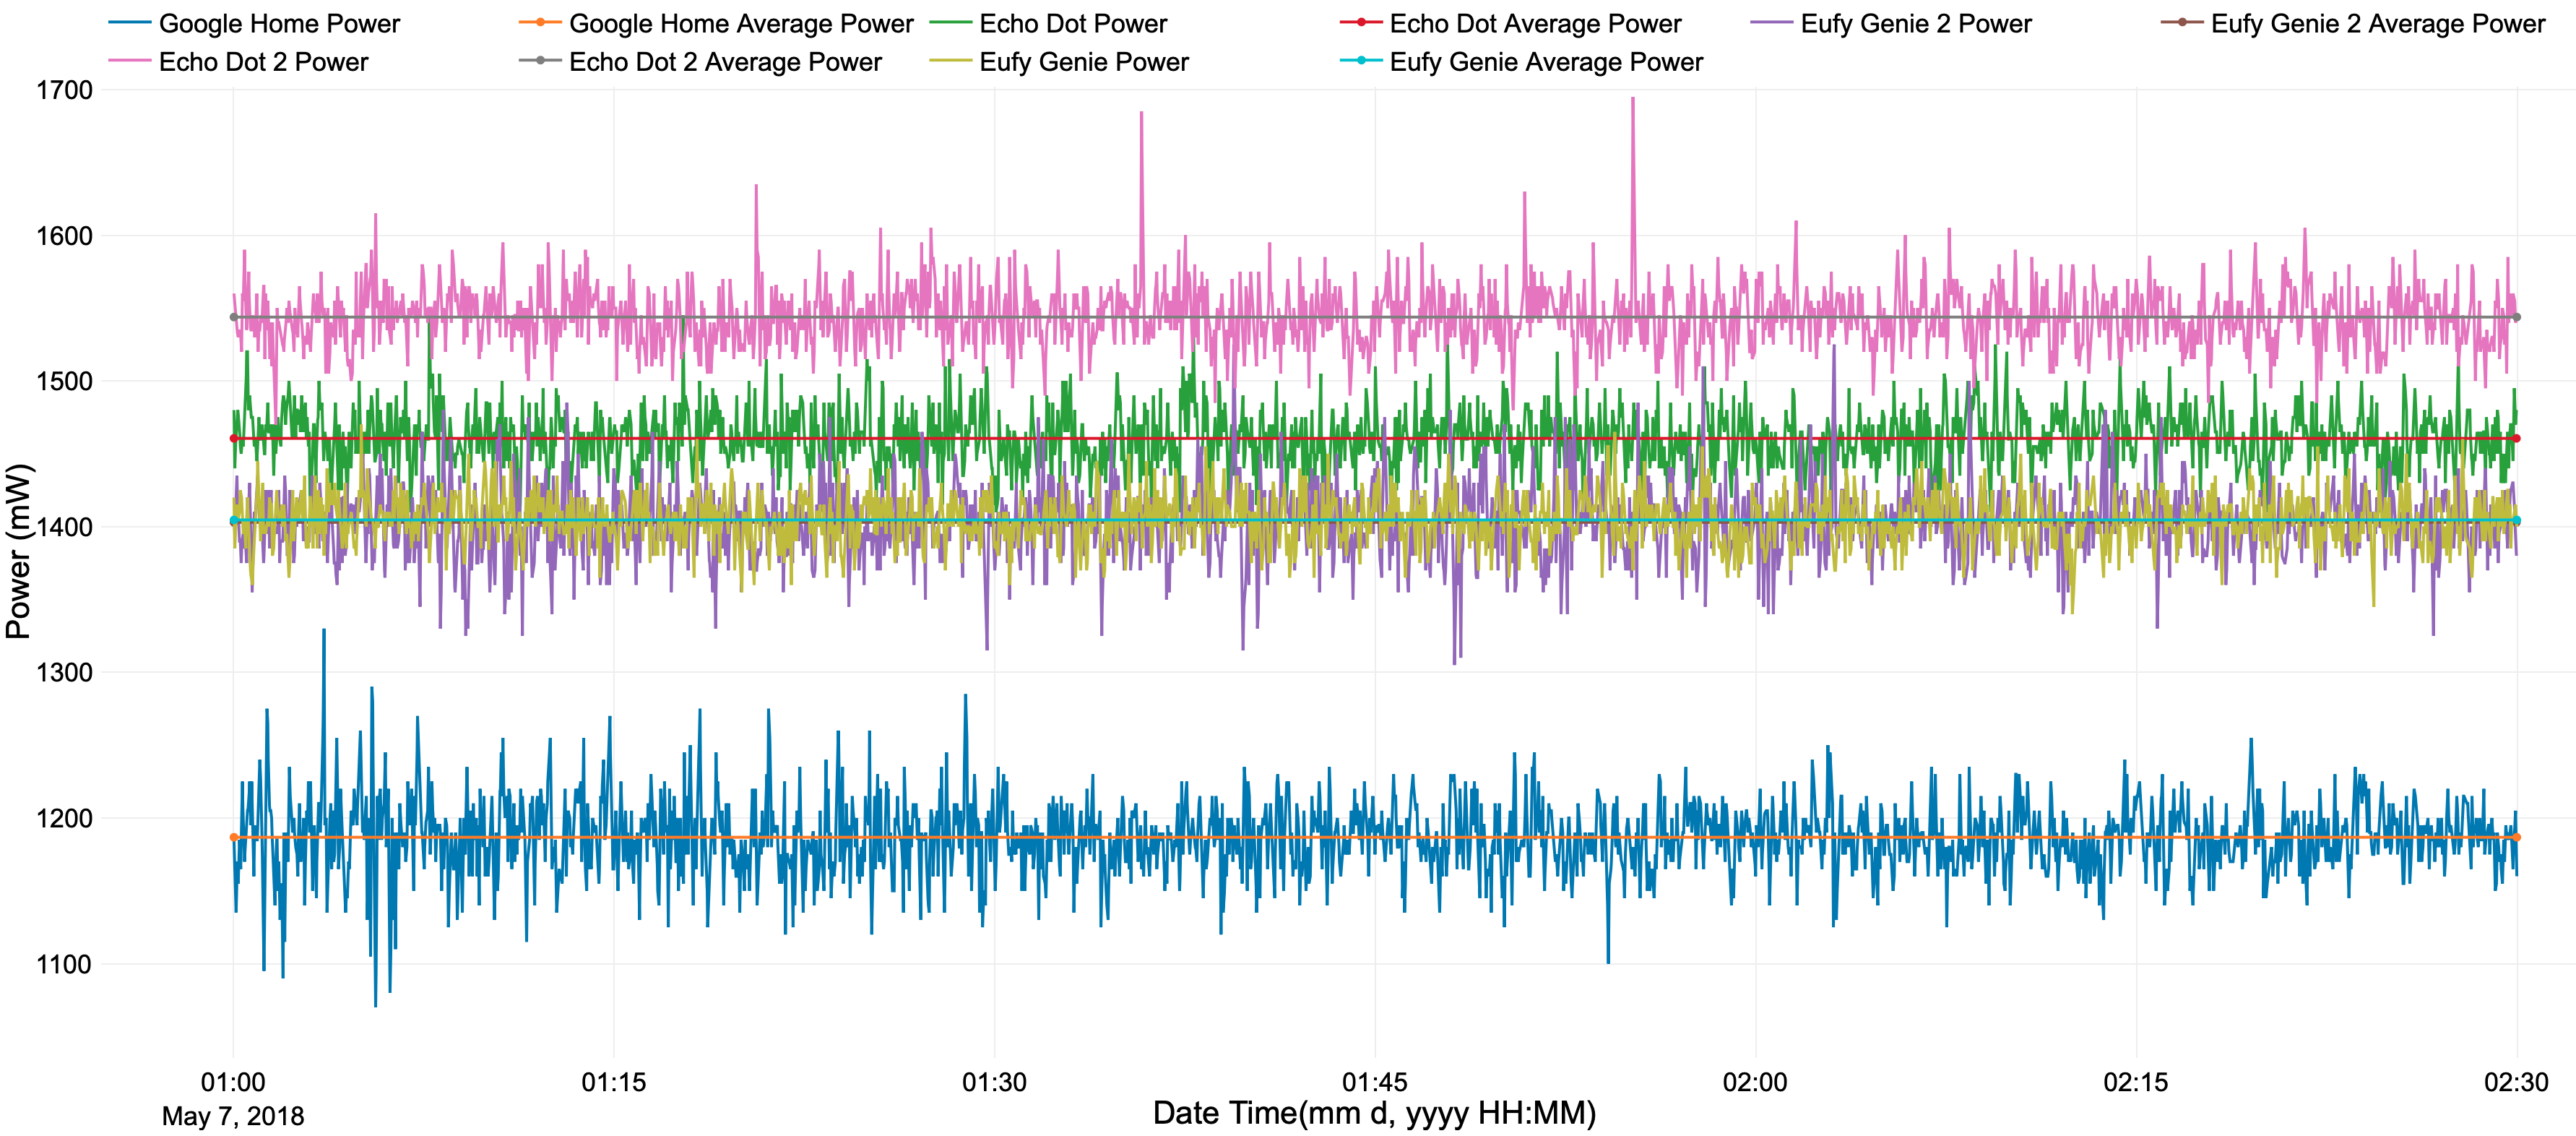
\includegraphics[width=1\textwidth]{baselineSpeakerPower.png}
    \caption{Baseline smart speaker power usage.}
    \label{fig:baselineSpeakerPower}
\end{figure}

\subsection{Smart Speaker Power Spikes When Asked for Weather}
\label{Smart Speaker Power Spikes When Asked for Weather}
This section continues to see if a smart speaker can be determined from power by focusing on power characteristics while the devices are in use. Figure \ref{fig:speakerWeatherSeperate} shows the power data where each device is asked for the weather four times.

In Figure \ref{fig:speakerWeatherSeperate} there is a visual spike for each device while it is giving the weather forecast. Each device is highlighted while in use. The Google Home was queried for the weather five times and thus contains an extra spike. From this data, we can note a Eufy trace has 400 mW peak to peak spikes, the Google Home has 600 mW peak to peak spikes, and the Echo Dot has 2,100 mW peak to peak spikes. This difference in magnitude implies that a device can be determined from a power trace if the device is asked for the weather. The next section analyzes more use cases, and the traces are summed together to simulate a shared home powerline more closely.

\begin{figure}[H]
    \centering
    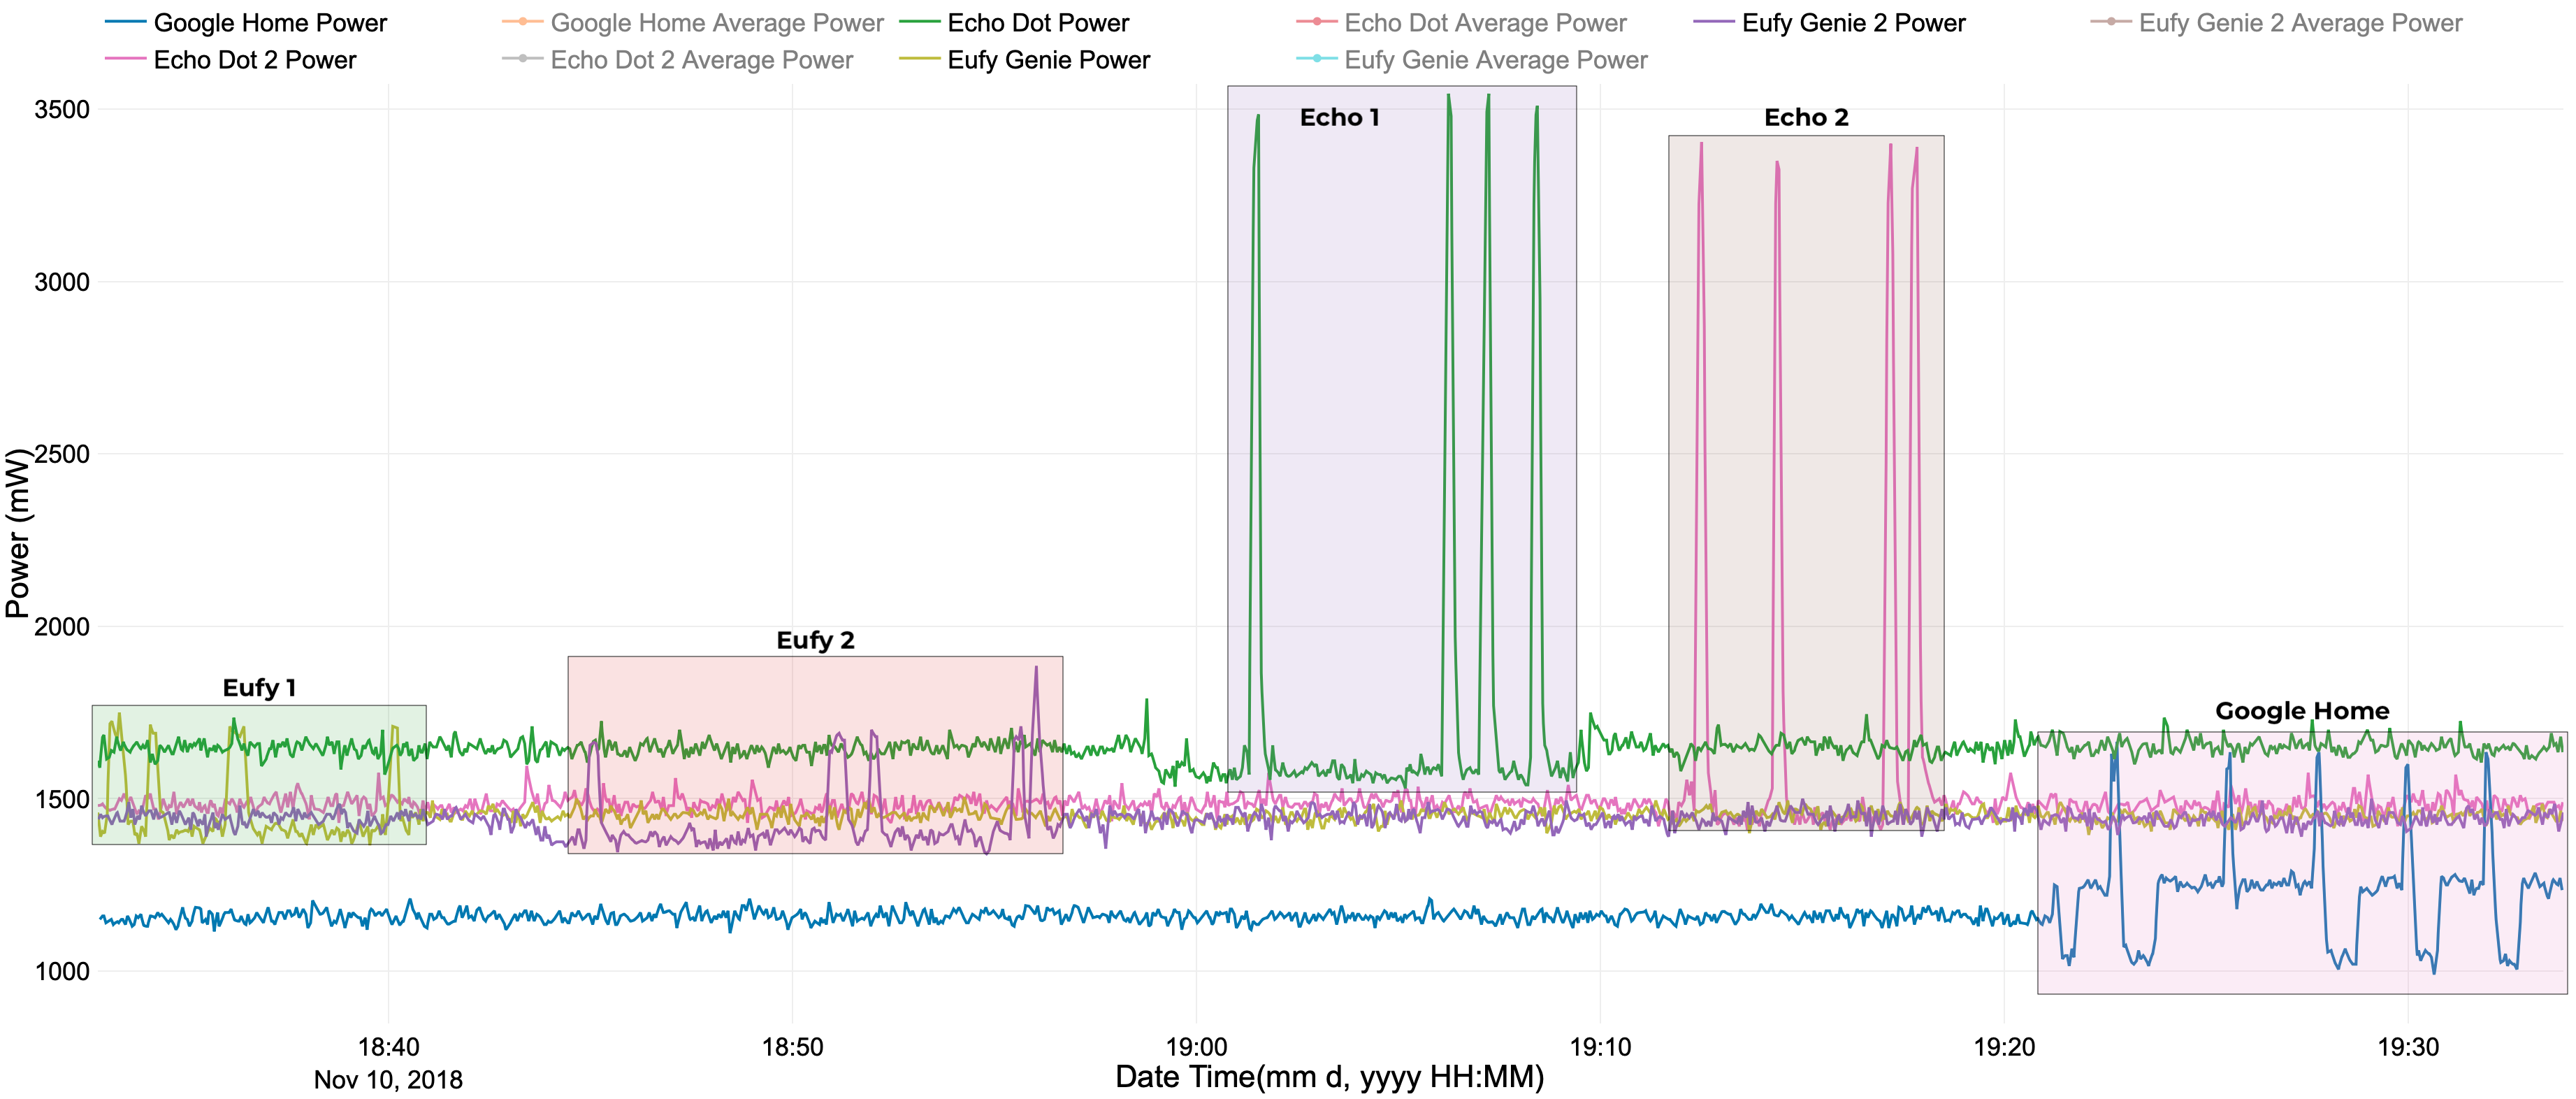
\includegraphics[width=1\textwidth]{speakerWeatherSeperate.png}
    \caption{Smart speakers' power usage when asked `what\'s the weather' four times.}
    \label{fig:speakerWeatherSeperate}
\end{figure}

\section{Summed Power Graph}
\label{sumPowerGraph}
This section attempts to analyze the power usage of all 5 of the smart speakers for different commands.

In Figure \ref{fig:weatherSum} we queried each smart speaker for the weather while all other smart speakers were muted at the 18:30 mark. We query each device 3-4 times for the weather. The Eufy had the smallest spike for the ``what is the weather'' command at 400 mW, then the Google Home at 600 mW, and finally the Echo Dot at 2000 mW, consistent with results in Section \ref{Smart Speaker Power Spikes When Asked for Weather}.

\begin{figure}[H]
  \centering
  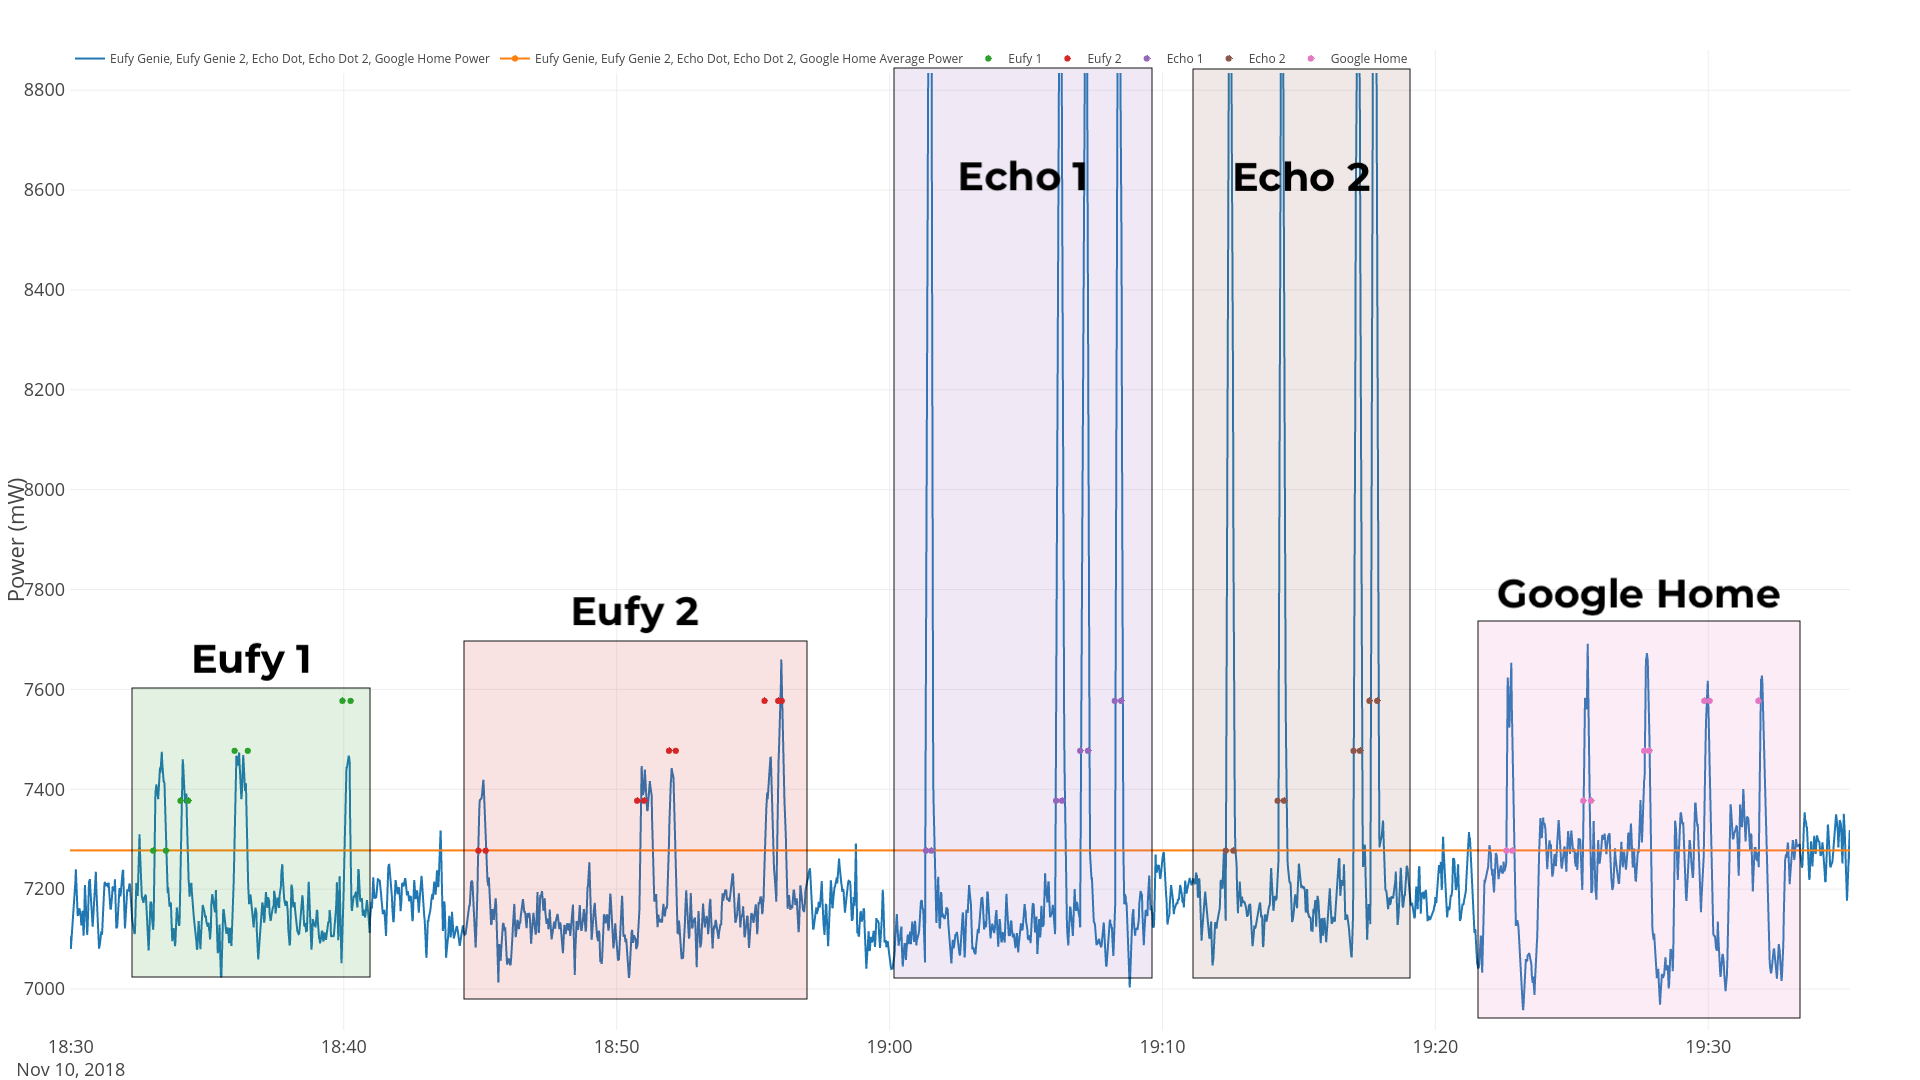
\includegraphics[width=1\textwidth]{figures/weatherSum.png}
  \caption{5 Smart Speakers Power Summed Together.}
  \label{fig:weatherSum}
\end{figure}

Figure \ref{fig:mixedNewsSum}, shows the smart speakers power usage when asked for the news. This graph and the rest of the summed graphs in this section use the same notation for signifying commands: Two dots of the same color on the same y-axis level signify the start and end of the command for a specific device.

In Figure \ref{fig:mixedNewsSum}, all devices have a spike at the beginning and end of the command and maintain a steady energy usage in between that is slightly higher than the idle energy used. The peak to peak spike of the Eufy Genie is the smallest at 350 mW, then the Google Home at 500 mW, and finally the Echo Dot at 1900 mW.

\begin{figure}[H]
  \centering
  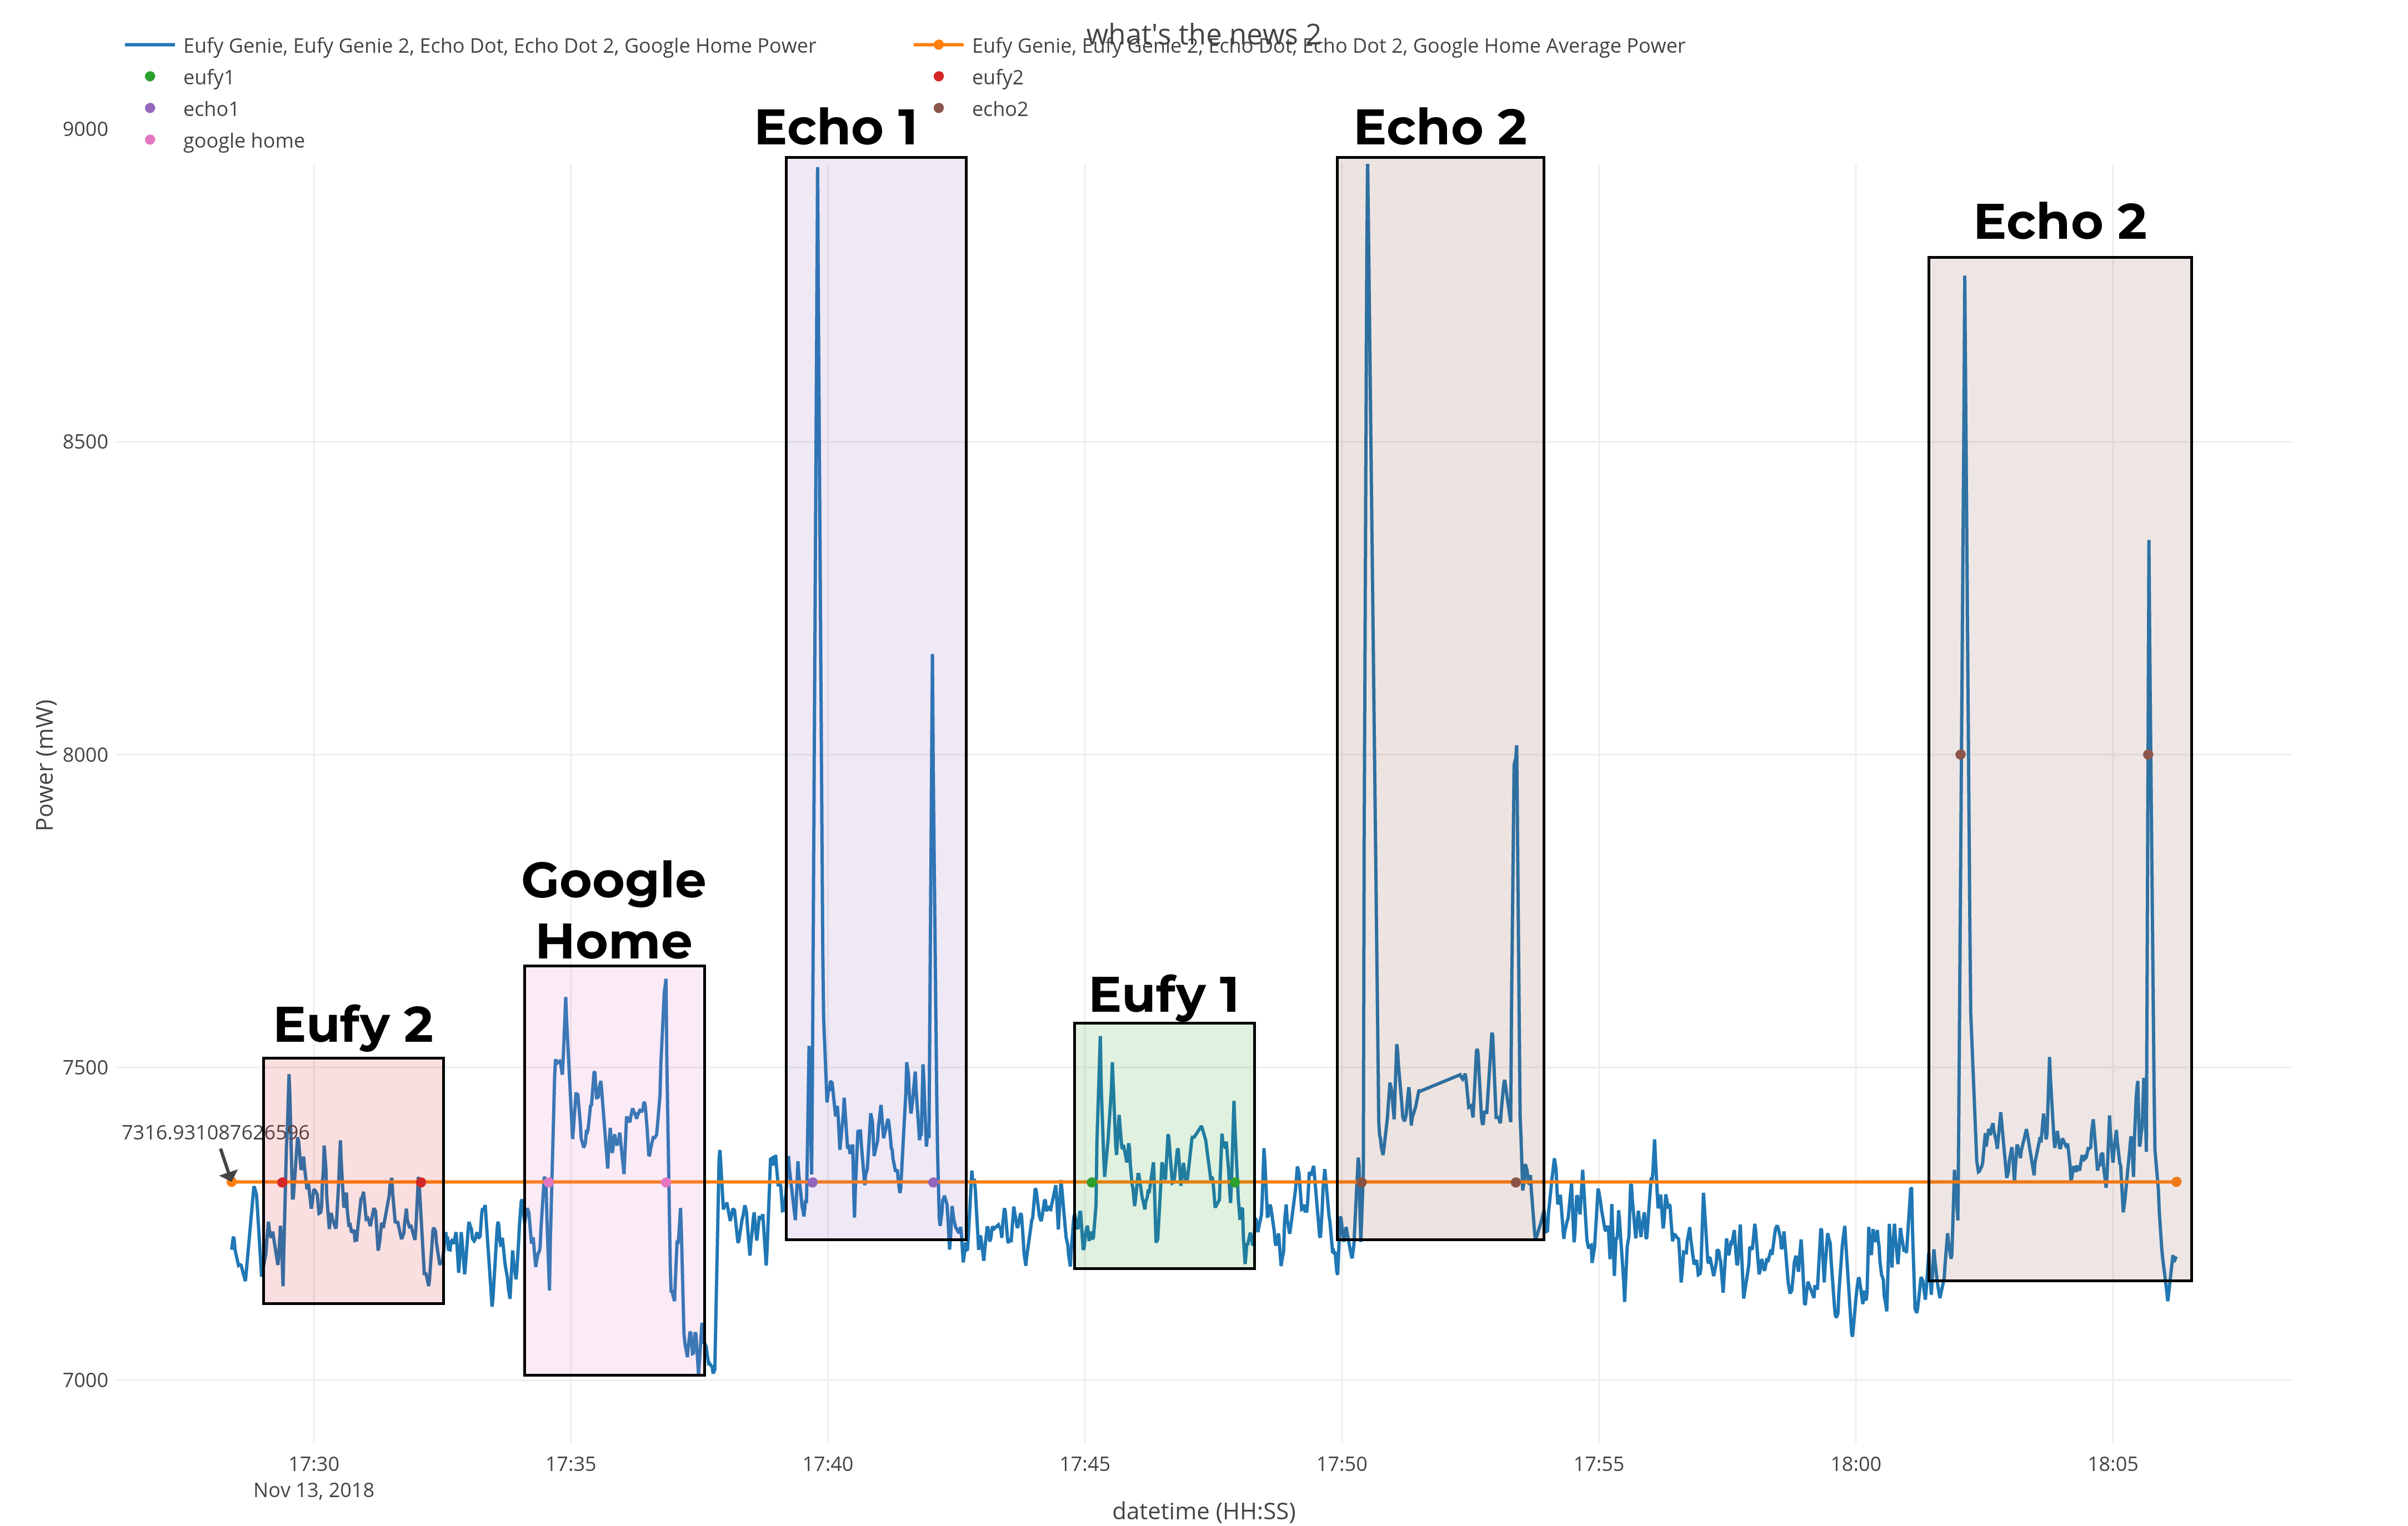
\includegraphics[width=1\textwidth]{figures/mixedNewsSum.png}
  \caption{5 Smart Speakers Power Summed Up. Queried each device for the news.}
  \label{fig:mixedNewsSum}
\end{figure}

Figure \ref{fig:bestBballSum} shows the smart speakers when asked for the best basketball player. The annotation scheme is the same as before. Each smart speaker is queried for the best basketball player in consecutive order four times. Like before, the Eufy has the smallest power spike at 420 mW peak to peak, the Google Home has a power Spike of 720 mW, and the Echo Dot has a power spike of 2180 mW.

When looking at graph \ref{fig:bestBballSum}, there is a power spike that is unaccounted for in correspondence to the event log at 18:12.

To figure what the power spike at 18:12 is, we separated the graphs into individual power traces as shown in Figure \ref{fig:bestBballSeperate}. From this graph, the power spike at 18:12 is attributed to the Echo Dot 2 because it is the only trace with a spike occurring. We then looked at the individual network usage for each of these devices in this time frame as shown in Figure \ref{fig:bestBballNetwork}. At 18:12, there is no significant network usage.

From Figures \ref{fig:bestBballSeperate} and \ref{fig:bestBballNetwork}, we speculate that because there is no network usage during this time but a power spike, the Echo Dot was briefly exposed to more light, causing the LEDs to brighten. The power usage before the spike and during the spike exactly match that of Figure \ref{fig:echolights}, starting at around 1500 mW, rising to about 2300 mW.

\begin{figure}[H]
  \centering
  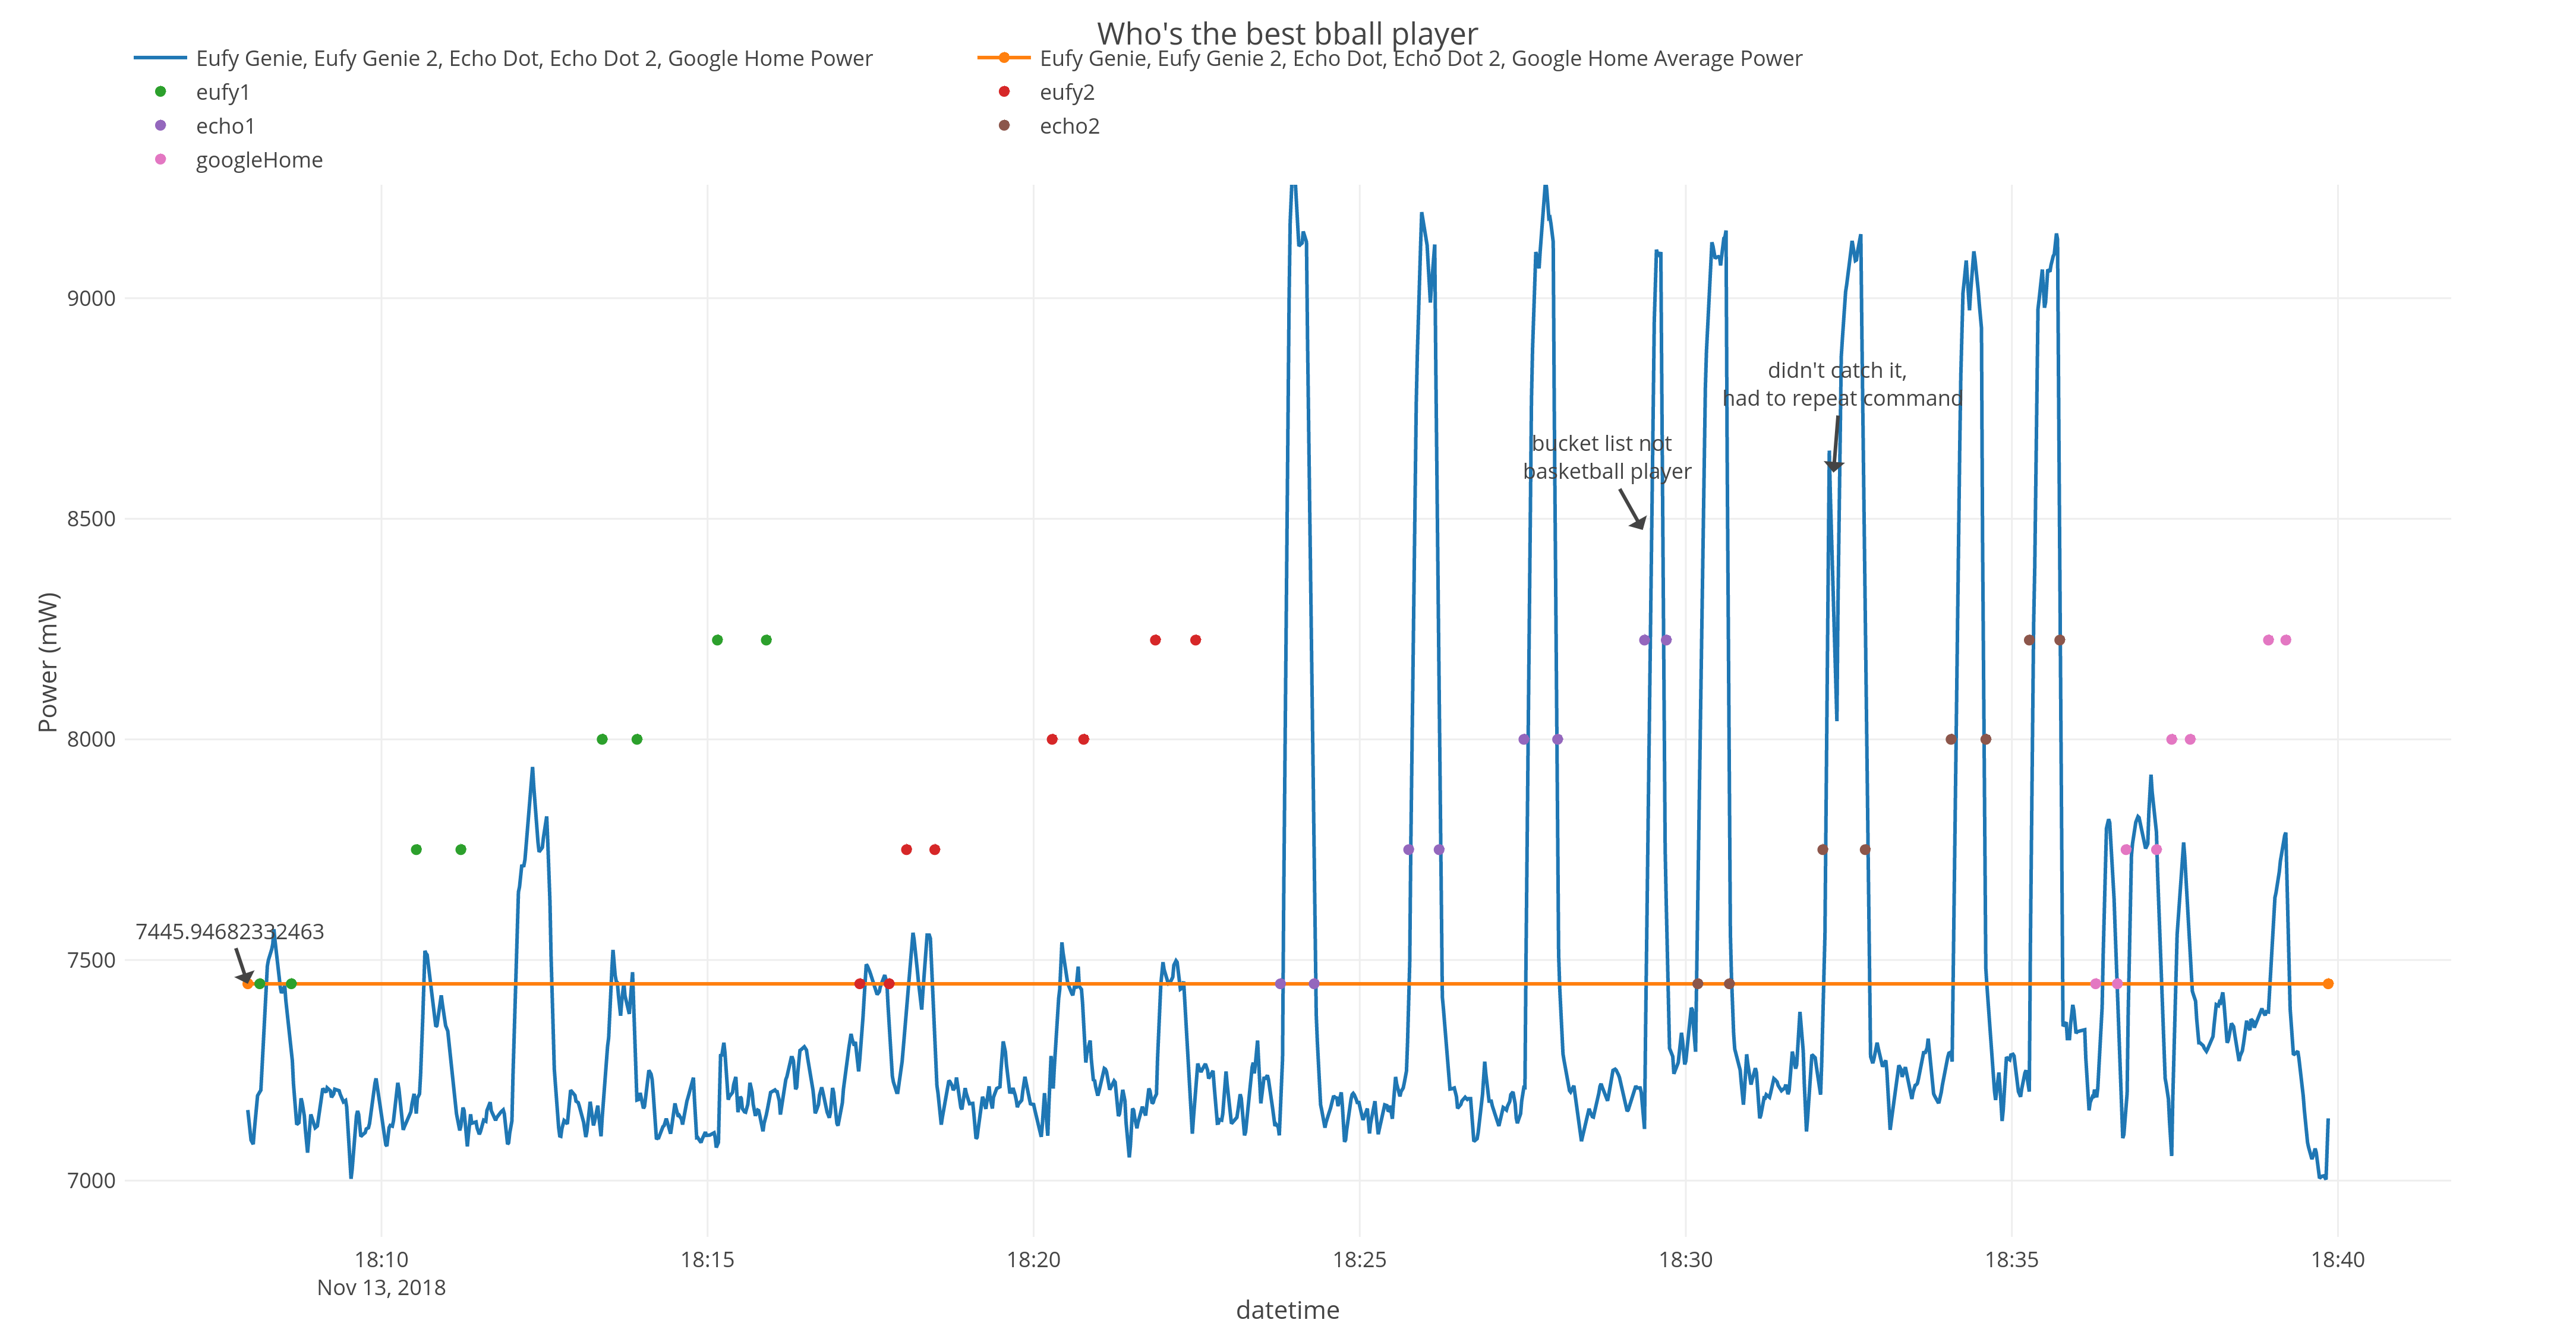
\includegraphics[width=1\textwidth]{figures/bestBballSum.png}
  \caption{5 Smart Speakers Power Summed Up. Queried each device for the
  best basketball player.}
  \label{fig:bestBballSum}
\end{figure}

\begin{figure}[H]
  \centering
  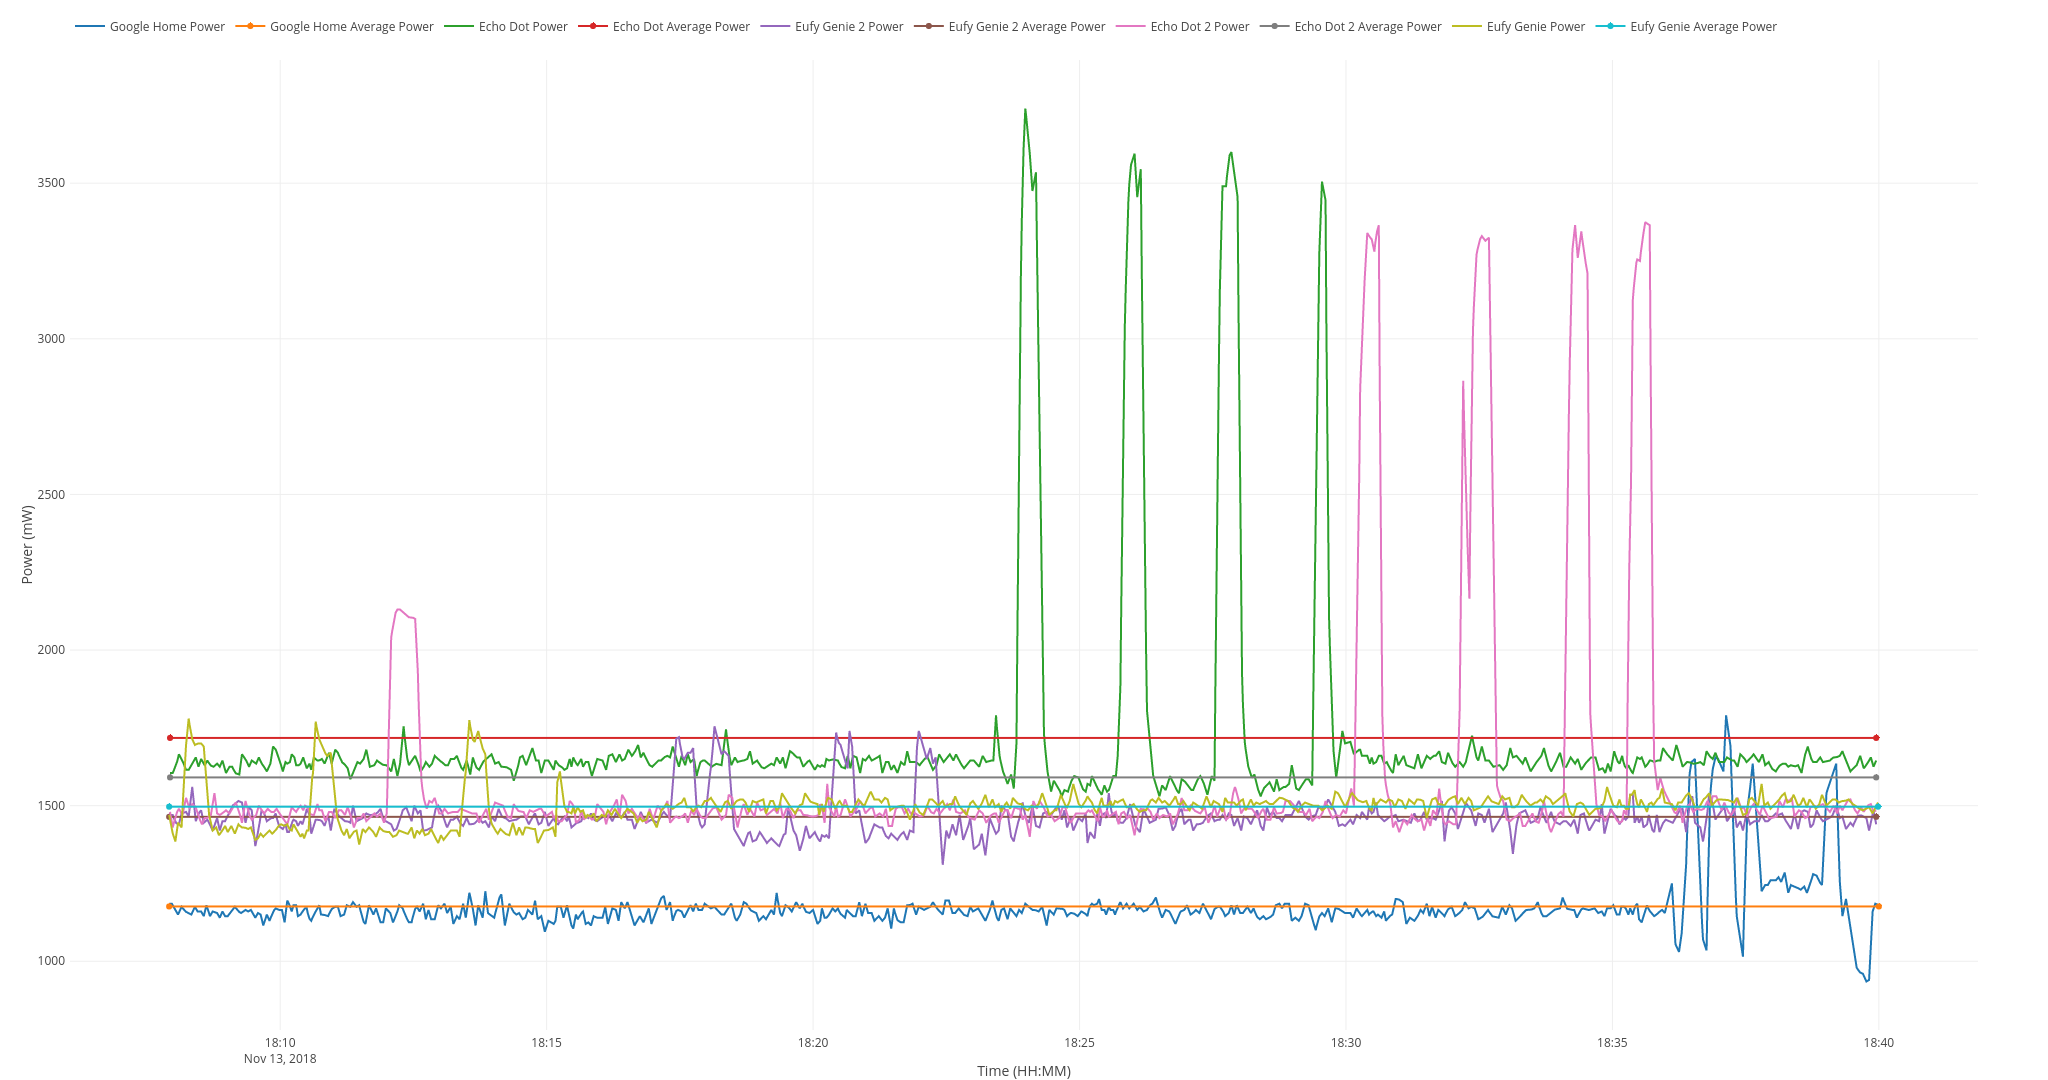
\includegraphics[width=1\textwidth]{figures/bestBballSeperate.png}
  \caption{5 Smart Speakers Power Usage over time. Queried each device for the
  best basketball player.}
  \label{fig:bestBballSeperate}
\end{figure}

\begin{figure}[H]
  \centering
  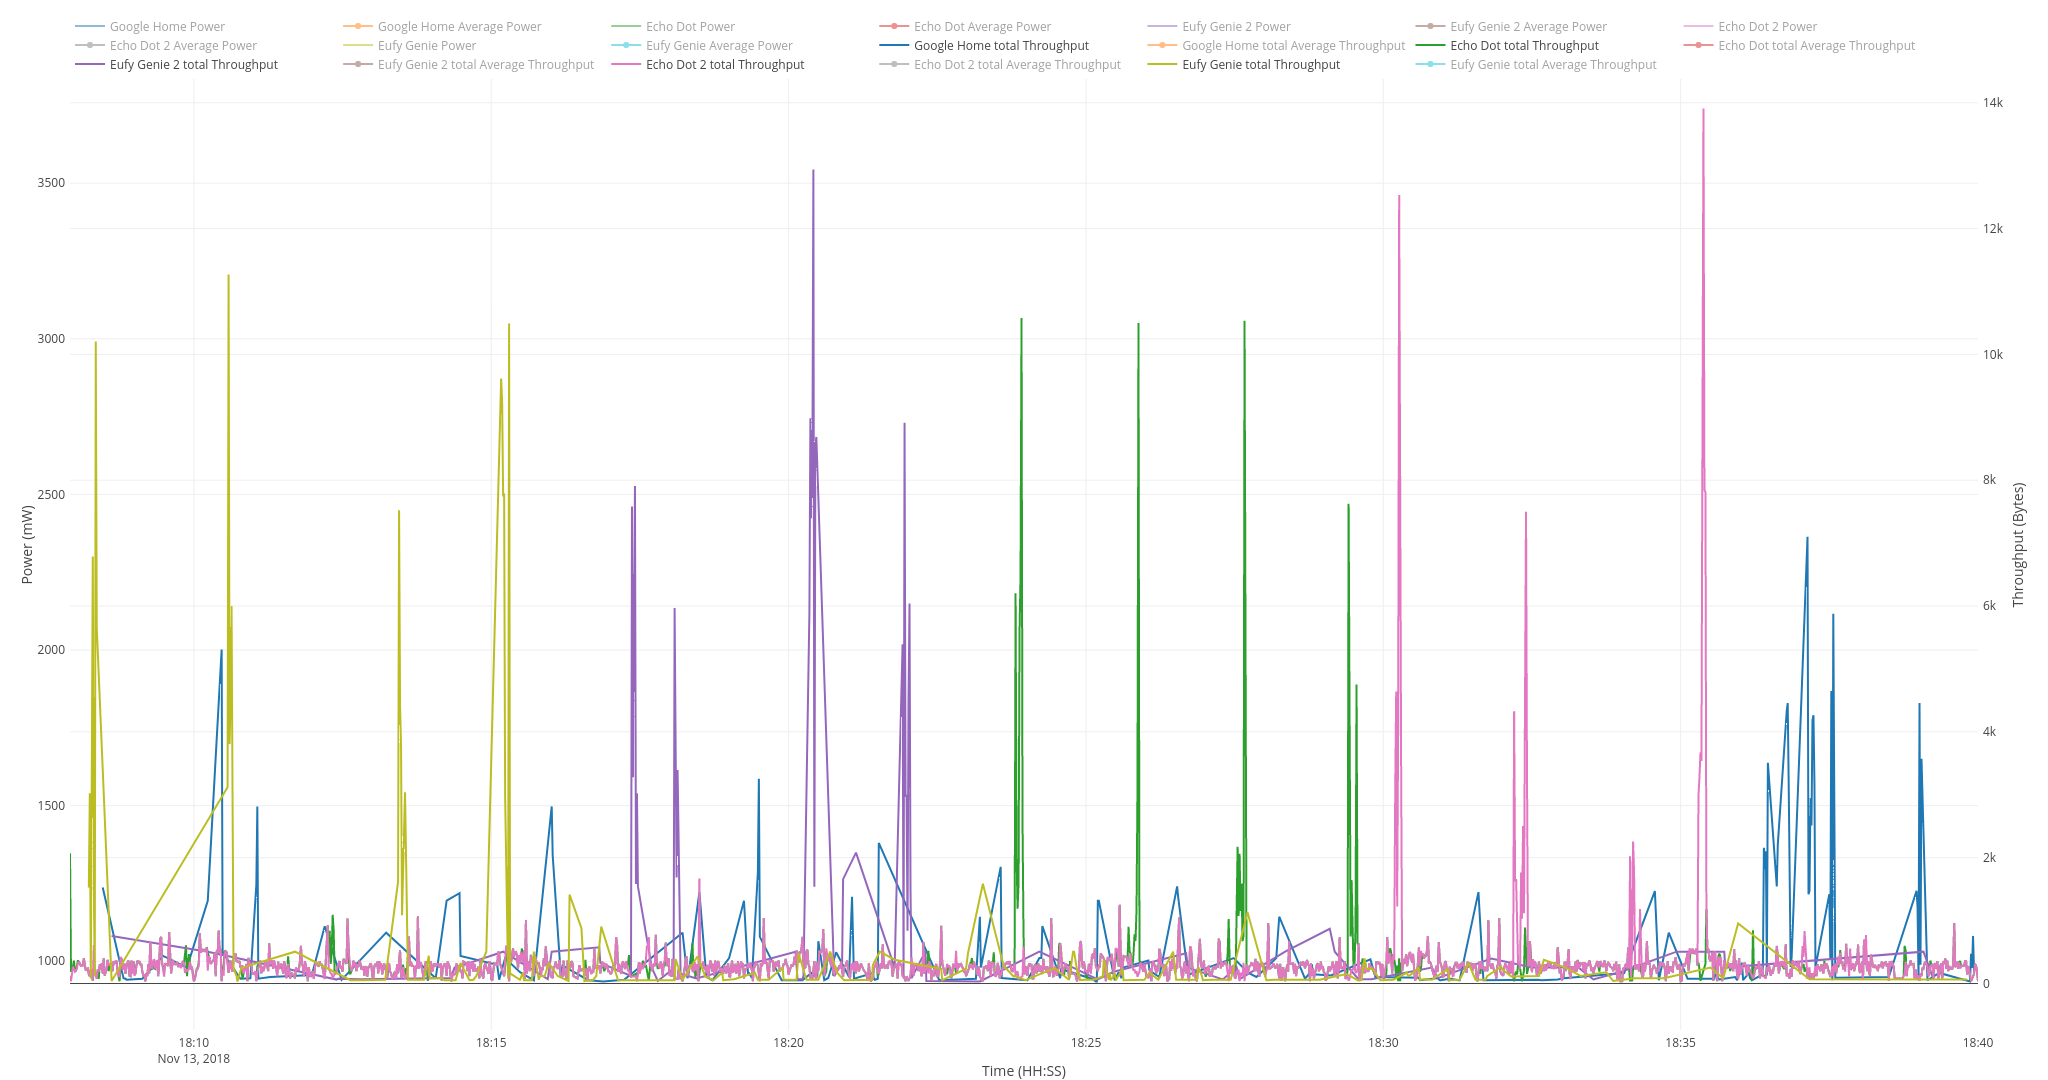
\includegraphics[width=1\textwidth]{figures/bestBballNetwork.png}
  \caption{5 Smart Speakers Network throughput over time. Queried each device for the best basketball player.}
  \label{fig:bestBballNetwork}
\end{figure}

Figure \ref{fig:spikeVoltages} shows the power spike averages for each query type (``what's the weather'' ``what's the news'', ``who's the best basketball player''). The black line at the top of each bar shows the standard deviation. Averaging peak to peak voltage spikes for each device across all commands shows the Eufy Genie with a 390 mW spike with 36.1 mW standard deviation, the Google Home with a 606.7 mW spike with 110 mW standard deviation, and the Echo Dot with a 2026.7 mW spike with 149.89 mW standard deviation.

Figure \ref{fig:spikeVoltages}, indicates that it is likely possible to determine a smart speaker from a shared power trace if a power spike occurs within the thresholds shown. From this, we conclude it is possible to determine a device model from visual examination of its power usage.

This is the first step to determine if it may be possible to see what devices are in use from analysis of someone's power line. But in a real house, there are more than just five smart speakers on a power line. The next step is to add noise from high power devices to see if it is still possible to visually determine the device in use from power spikes \ref{sumPowerGraphWithNoise}.

\begin{figure}[H]
  \centering
  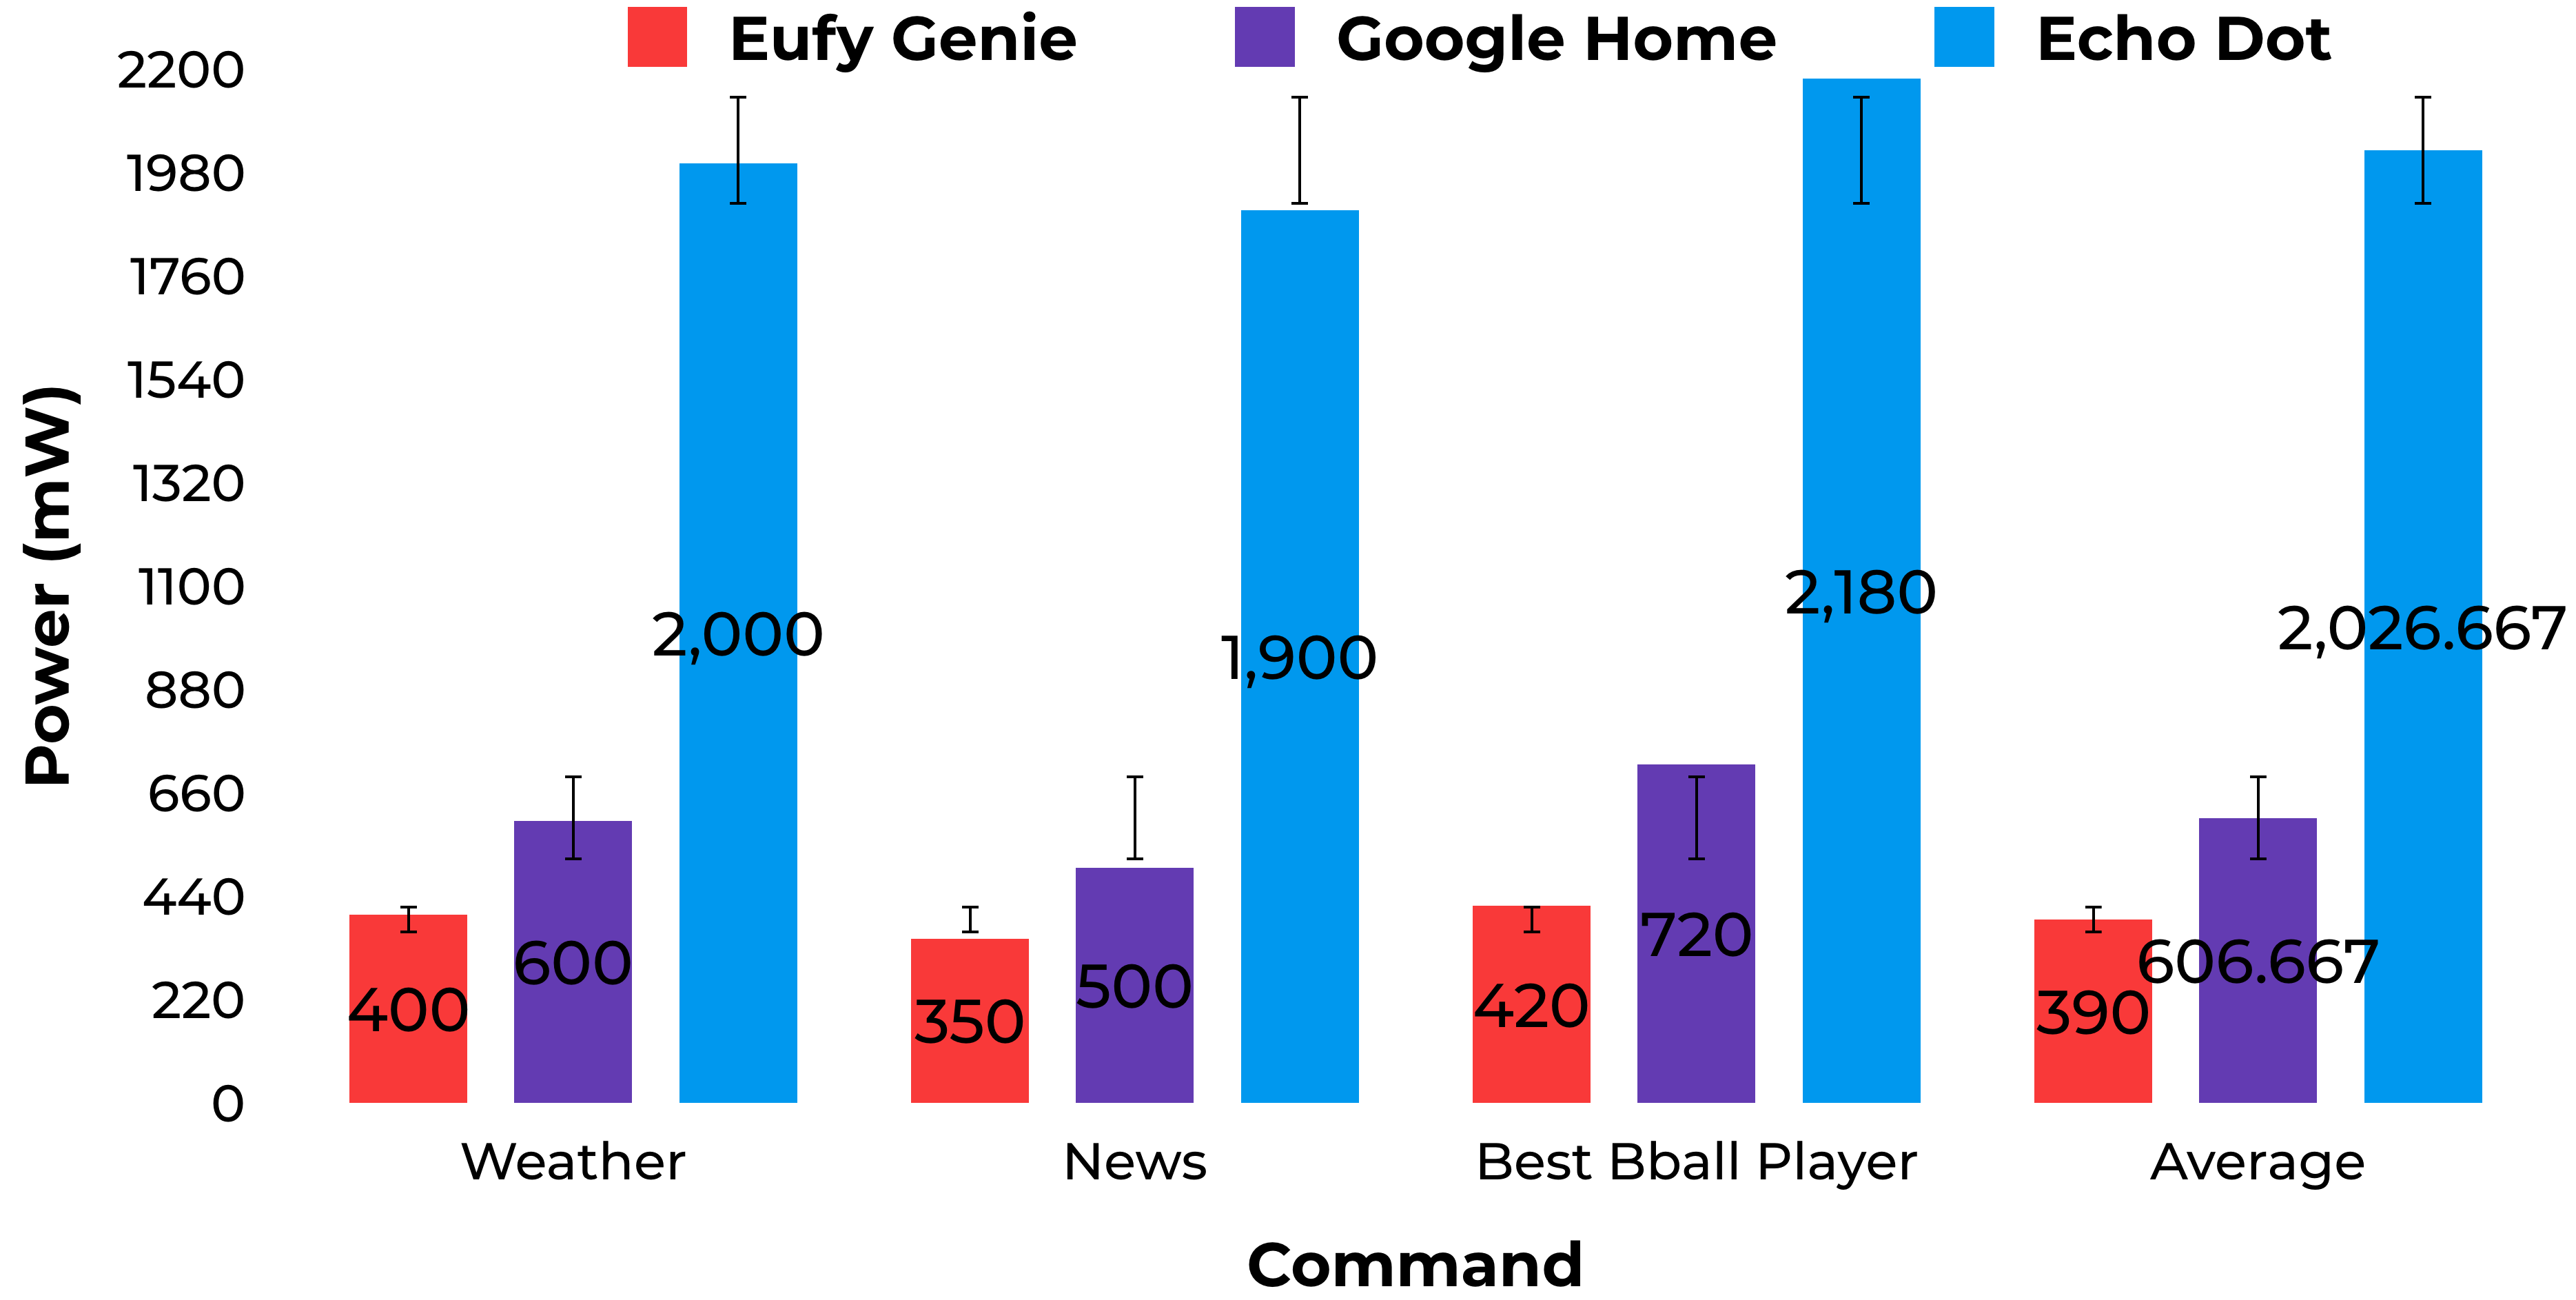
\includegraphics[width=1\textwidth]{figures/spikeVoltages.png}
  \caption{Spike summary of for each query.}
  \label{fig:spikeVoltages}
\end{figure}

\section{Summed Power Graph with Noise}
\label{sumPowerGraphWithNoise}
In this section, we introduce noise into the summed smart speaker setup so that we can determine if the power spike from each smart speaker is still discernible within a summed power graph when we add high power devices.

In each subsection, there are three traces. The first trace (blue trace) is the summed power usage of our five smart speakers (2 Echo Dots, 2 Eufy Genies, 1 Google Home) when asked for the best basketball player four times. This is the same trace as shown in Figure \ref{fig:bestBballSum}. The second trace (purple trace) is the power usage of a high power device. It maps to various devices as we switch them out. The third trace (red trace) is the sum of both trace 1 and 2.

The X-axis is the time elapsed in seconds rather than a specific time stamp because the smart speaker trace and `noise' trace are in different time frames. The Y-axis is the power used by each device at that time.

Figure \ref{fig:fanIdleSeperate} shows an example of the traces used separately. This is shown separately at first, but are summed together for the rest of the paper so that the scale of the noise can be understood.

\begin{figure}[H]
  \centering
  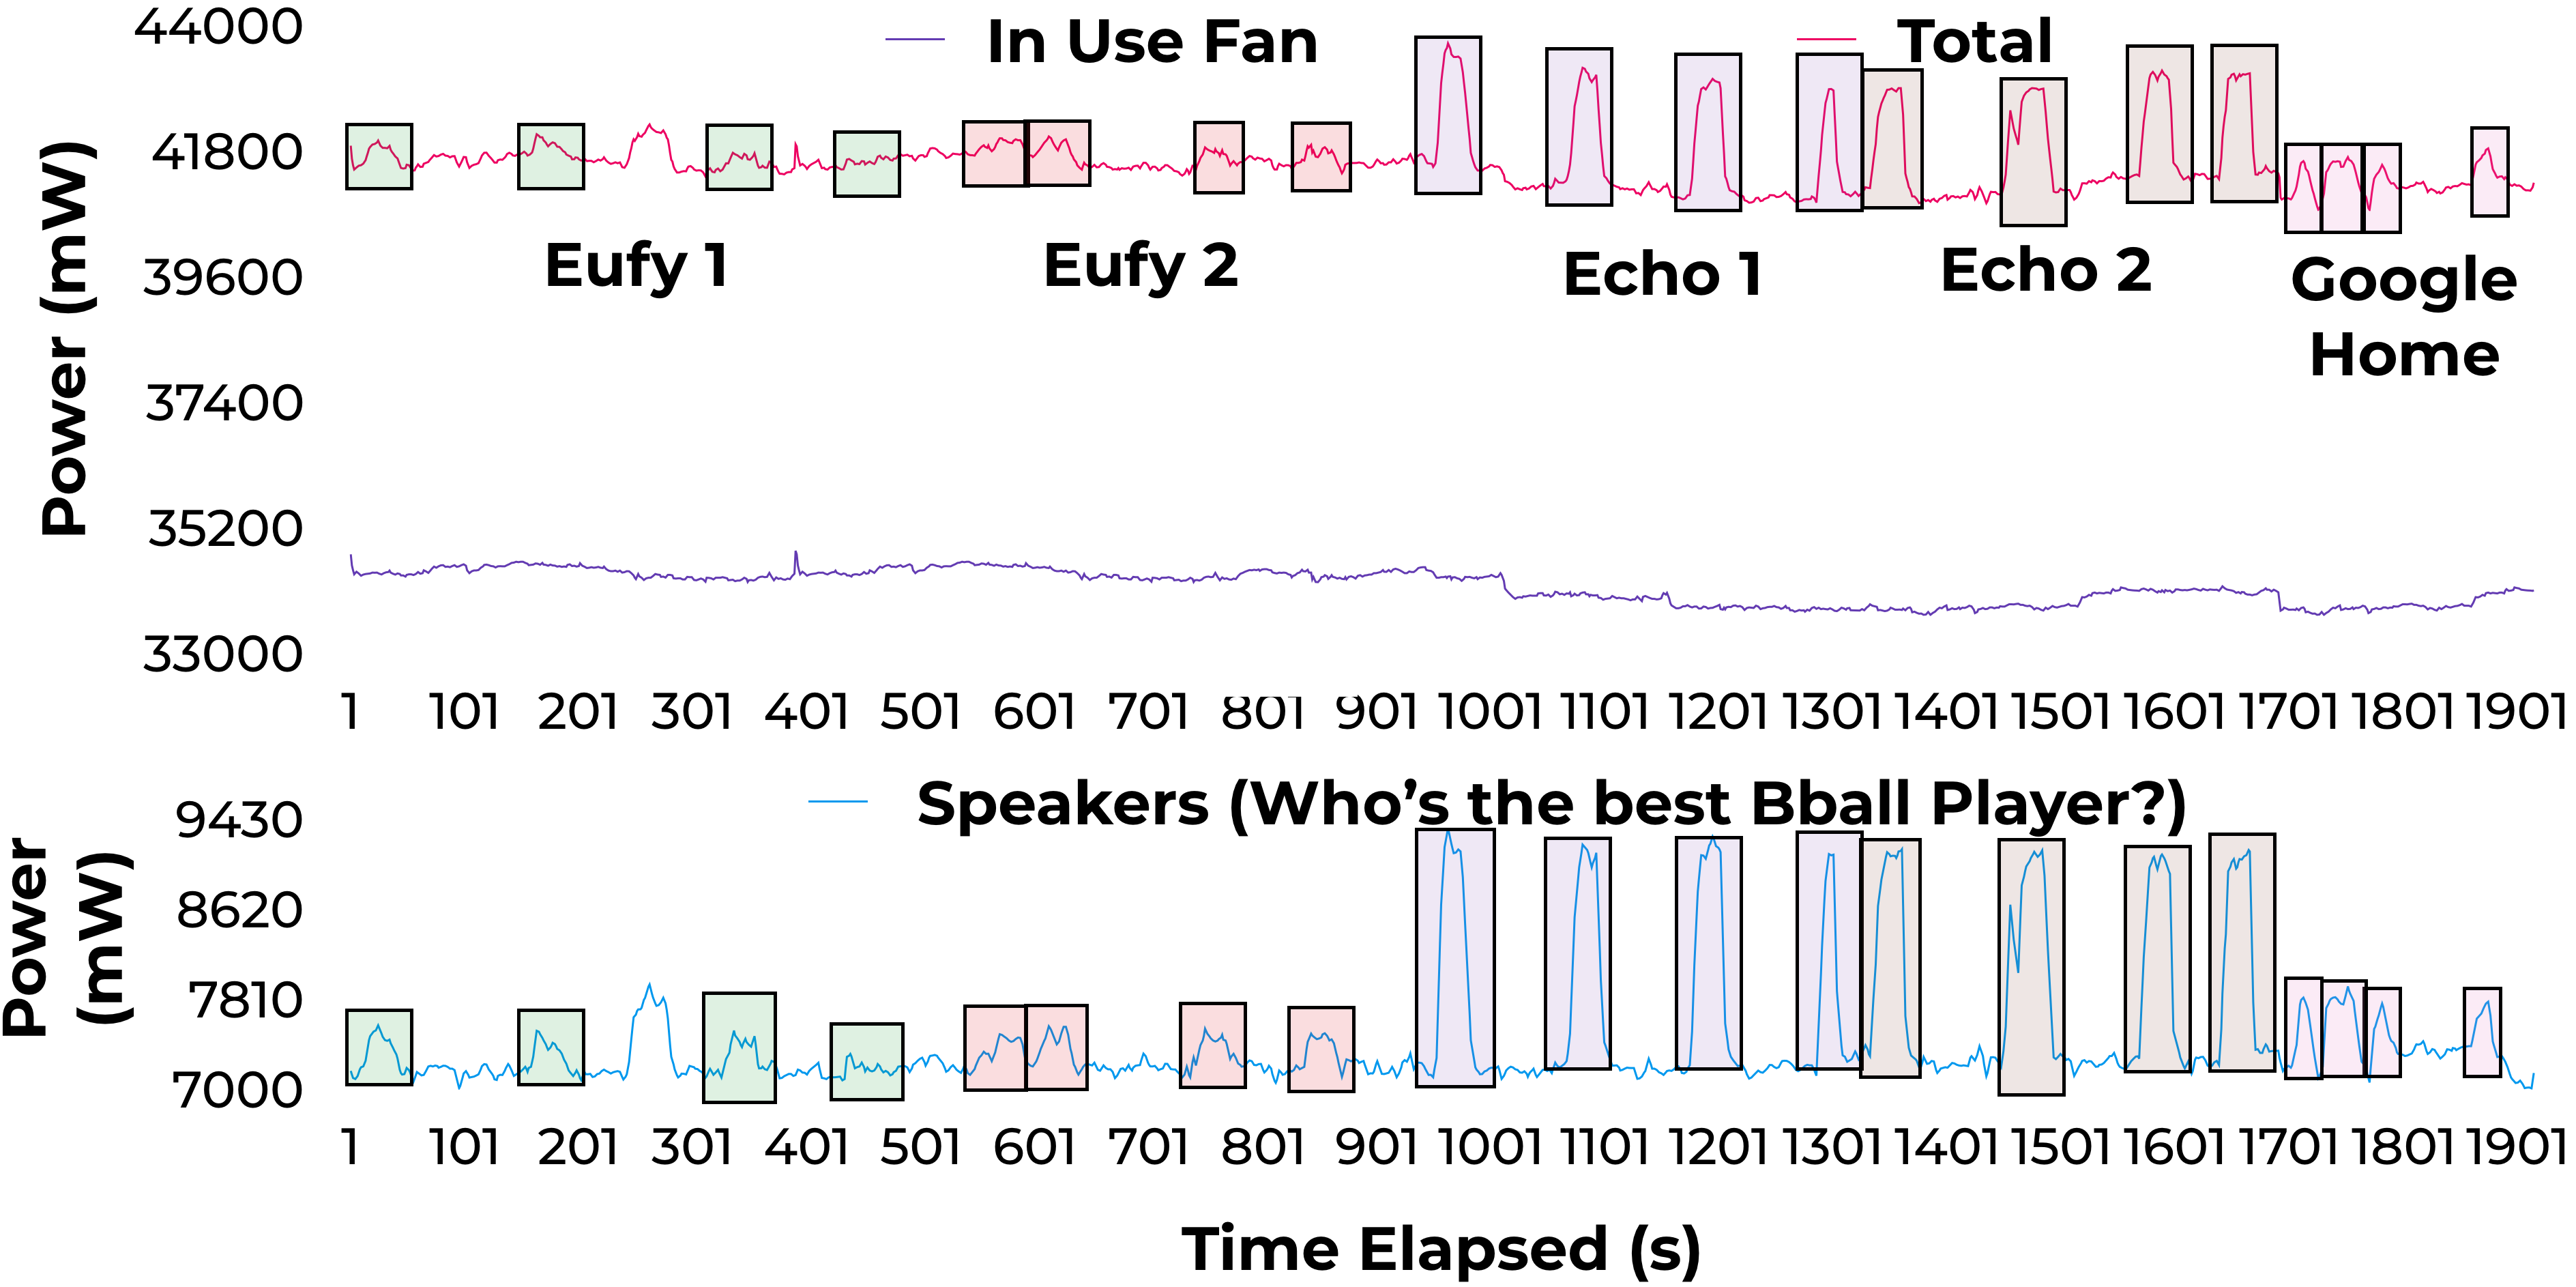
\includegraphics[width=1\textwidth]{figures/inUseFanNoiseSeperate.png}
  \caption{Figure \ref{fig:bestBballSum} summed smart speaker power, in use fan noise, and total power shown separately.}
  \label{fig:fanIdleSeperate}
\end{figure}

Figures \ref{fig:fanIdleSeperate}, \ref{fig:fanIdle}, \ref{fig:uWaveIdle}, \ref{fig:fridgeIdle}, \ref{fig:nucIdle}, and \ref{fig:allIdleNoise}show the smart speaker power trace when asked for the best basketball player with noise from a PC (Intel NUC), fan, refrigerator, or microwave. In these graphs, high power devices are in idle or steady power state. Then Figures \ref{fig:uWaveInUse}, \ref{fig:fridgeInUse}, and \ref{fig:nucInUse} show noise from the high power devices while in use, introducing noise that make visual detection of smart speakers more difficult.

\begin{figure}[H]
  \centering
  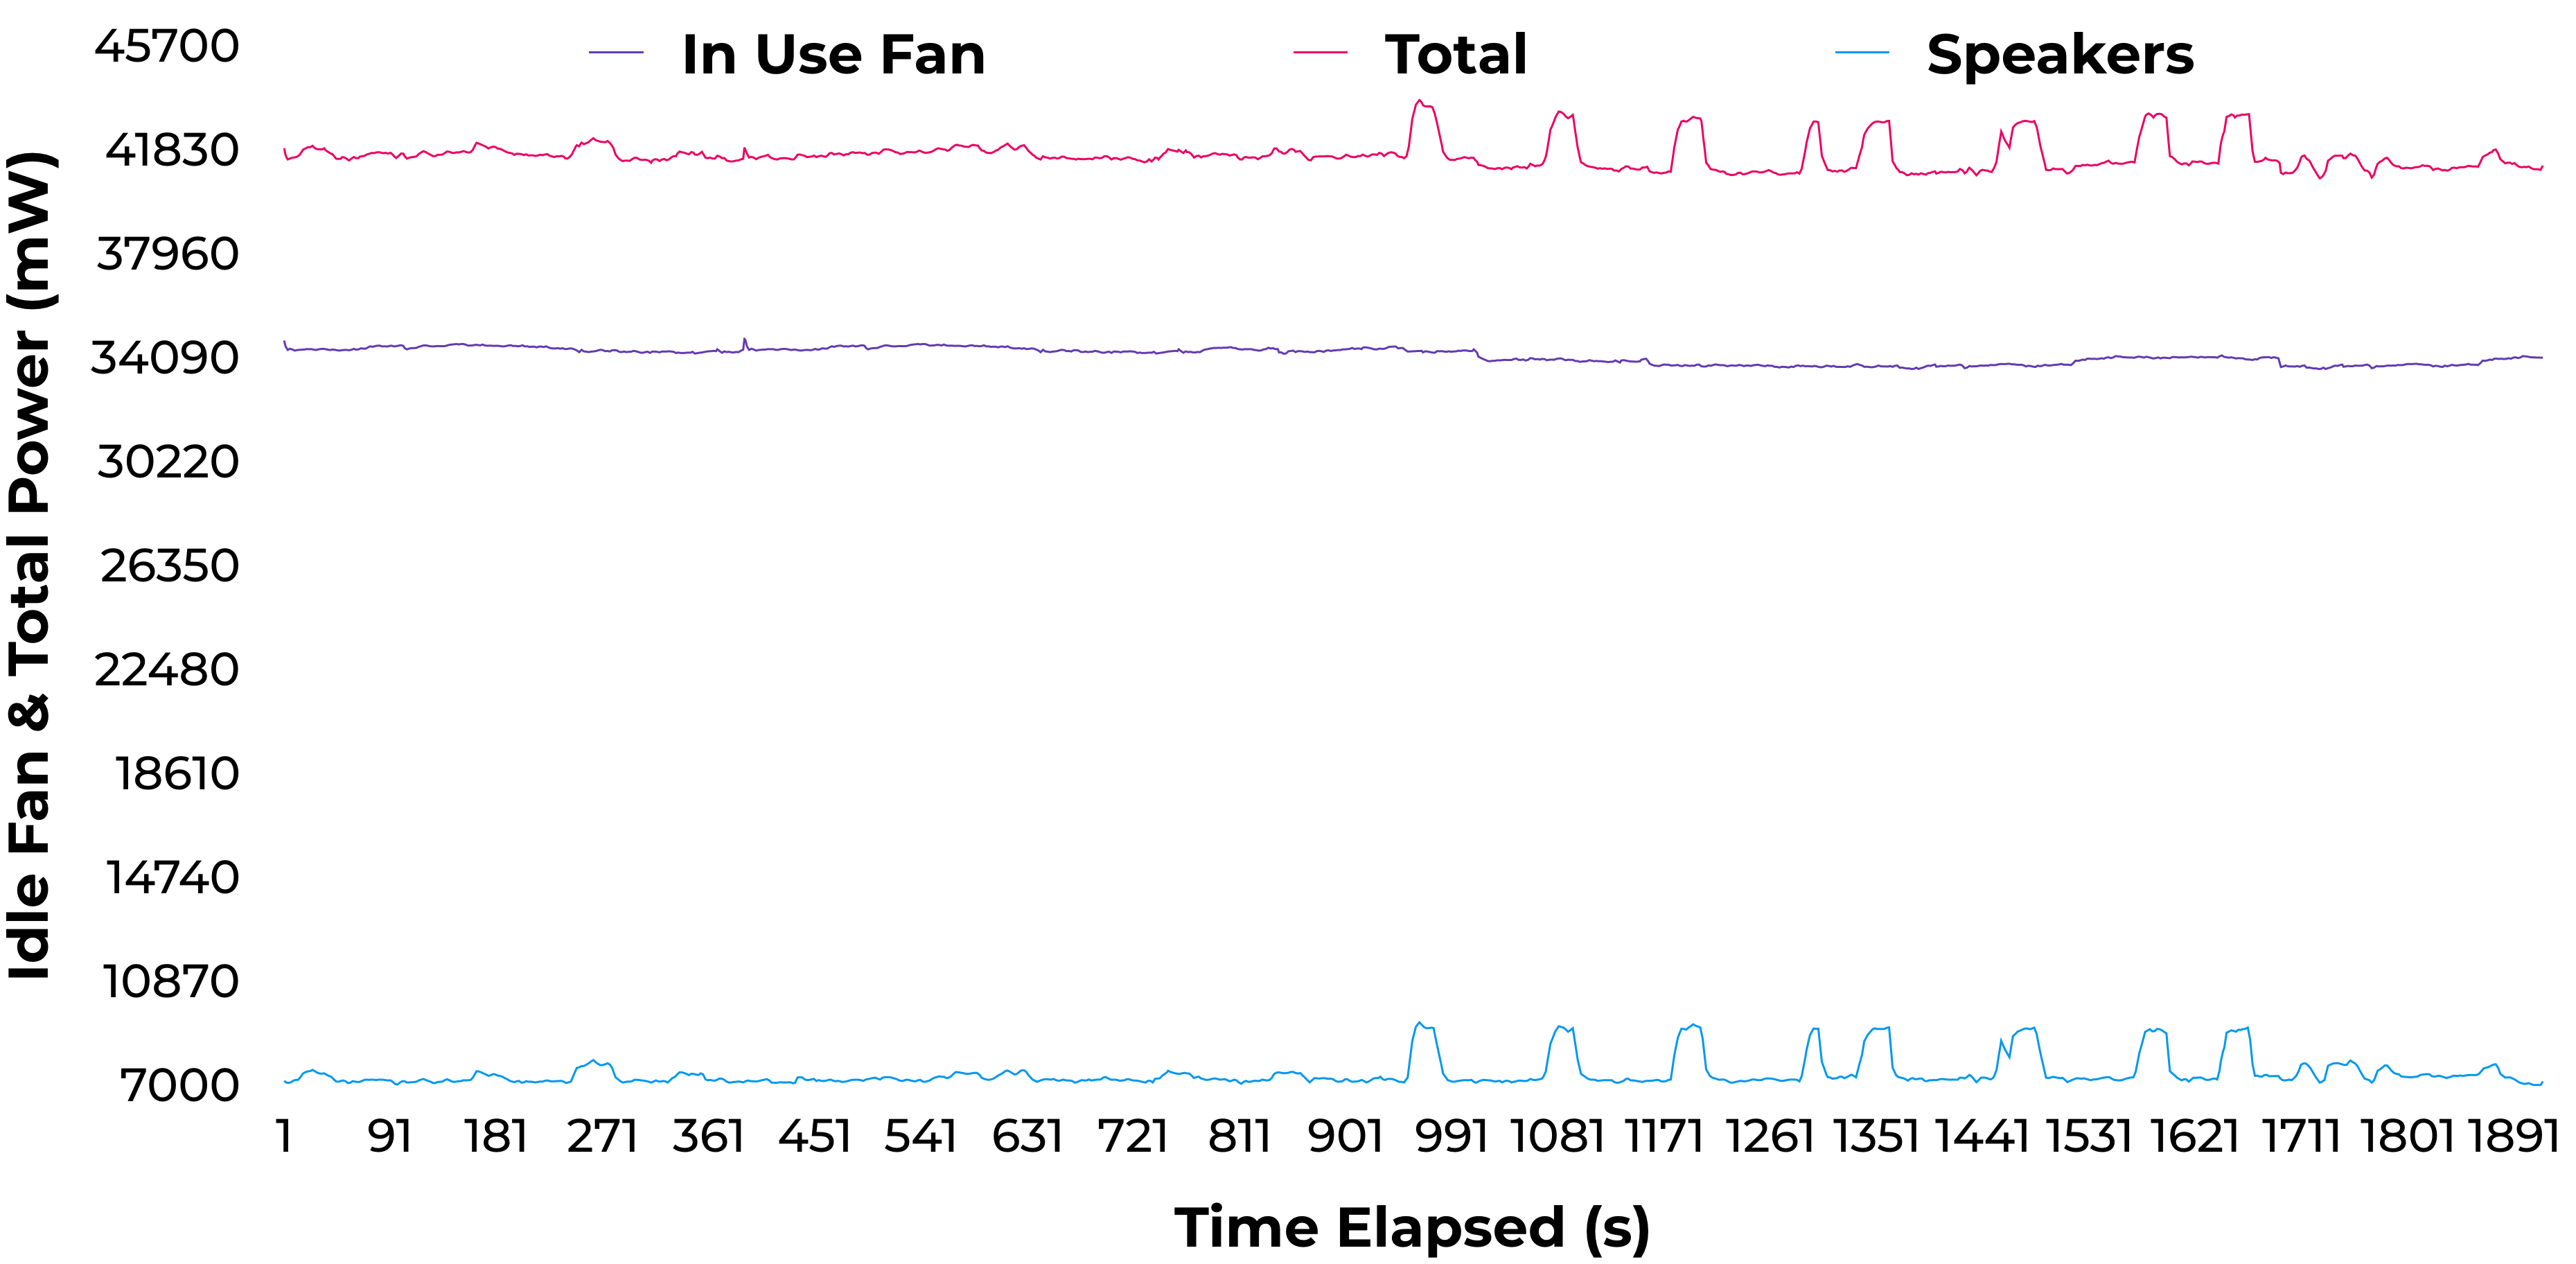
\includegraphics[width=1\textwidth]{figures/inUseFanNoise.png}
  \caption{Figure \ref{fig:bestBballSum} summed smart speaker power, in use fan noise, and total power.}
  \label{fig:fanIdle}
\end{figure}

\begin{figure}[H]
  \centering
  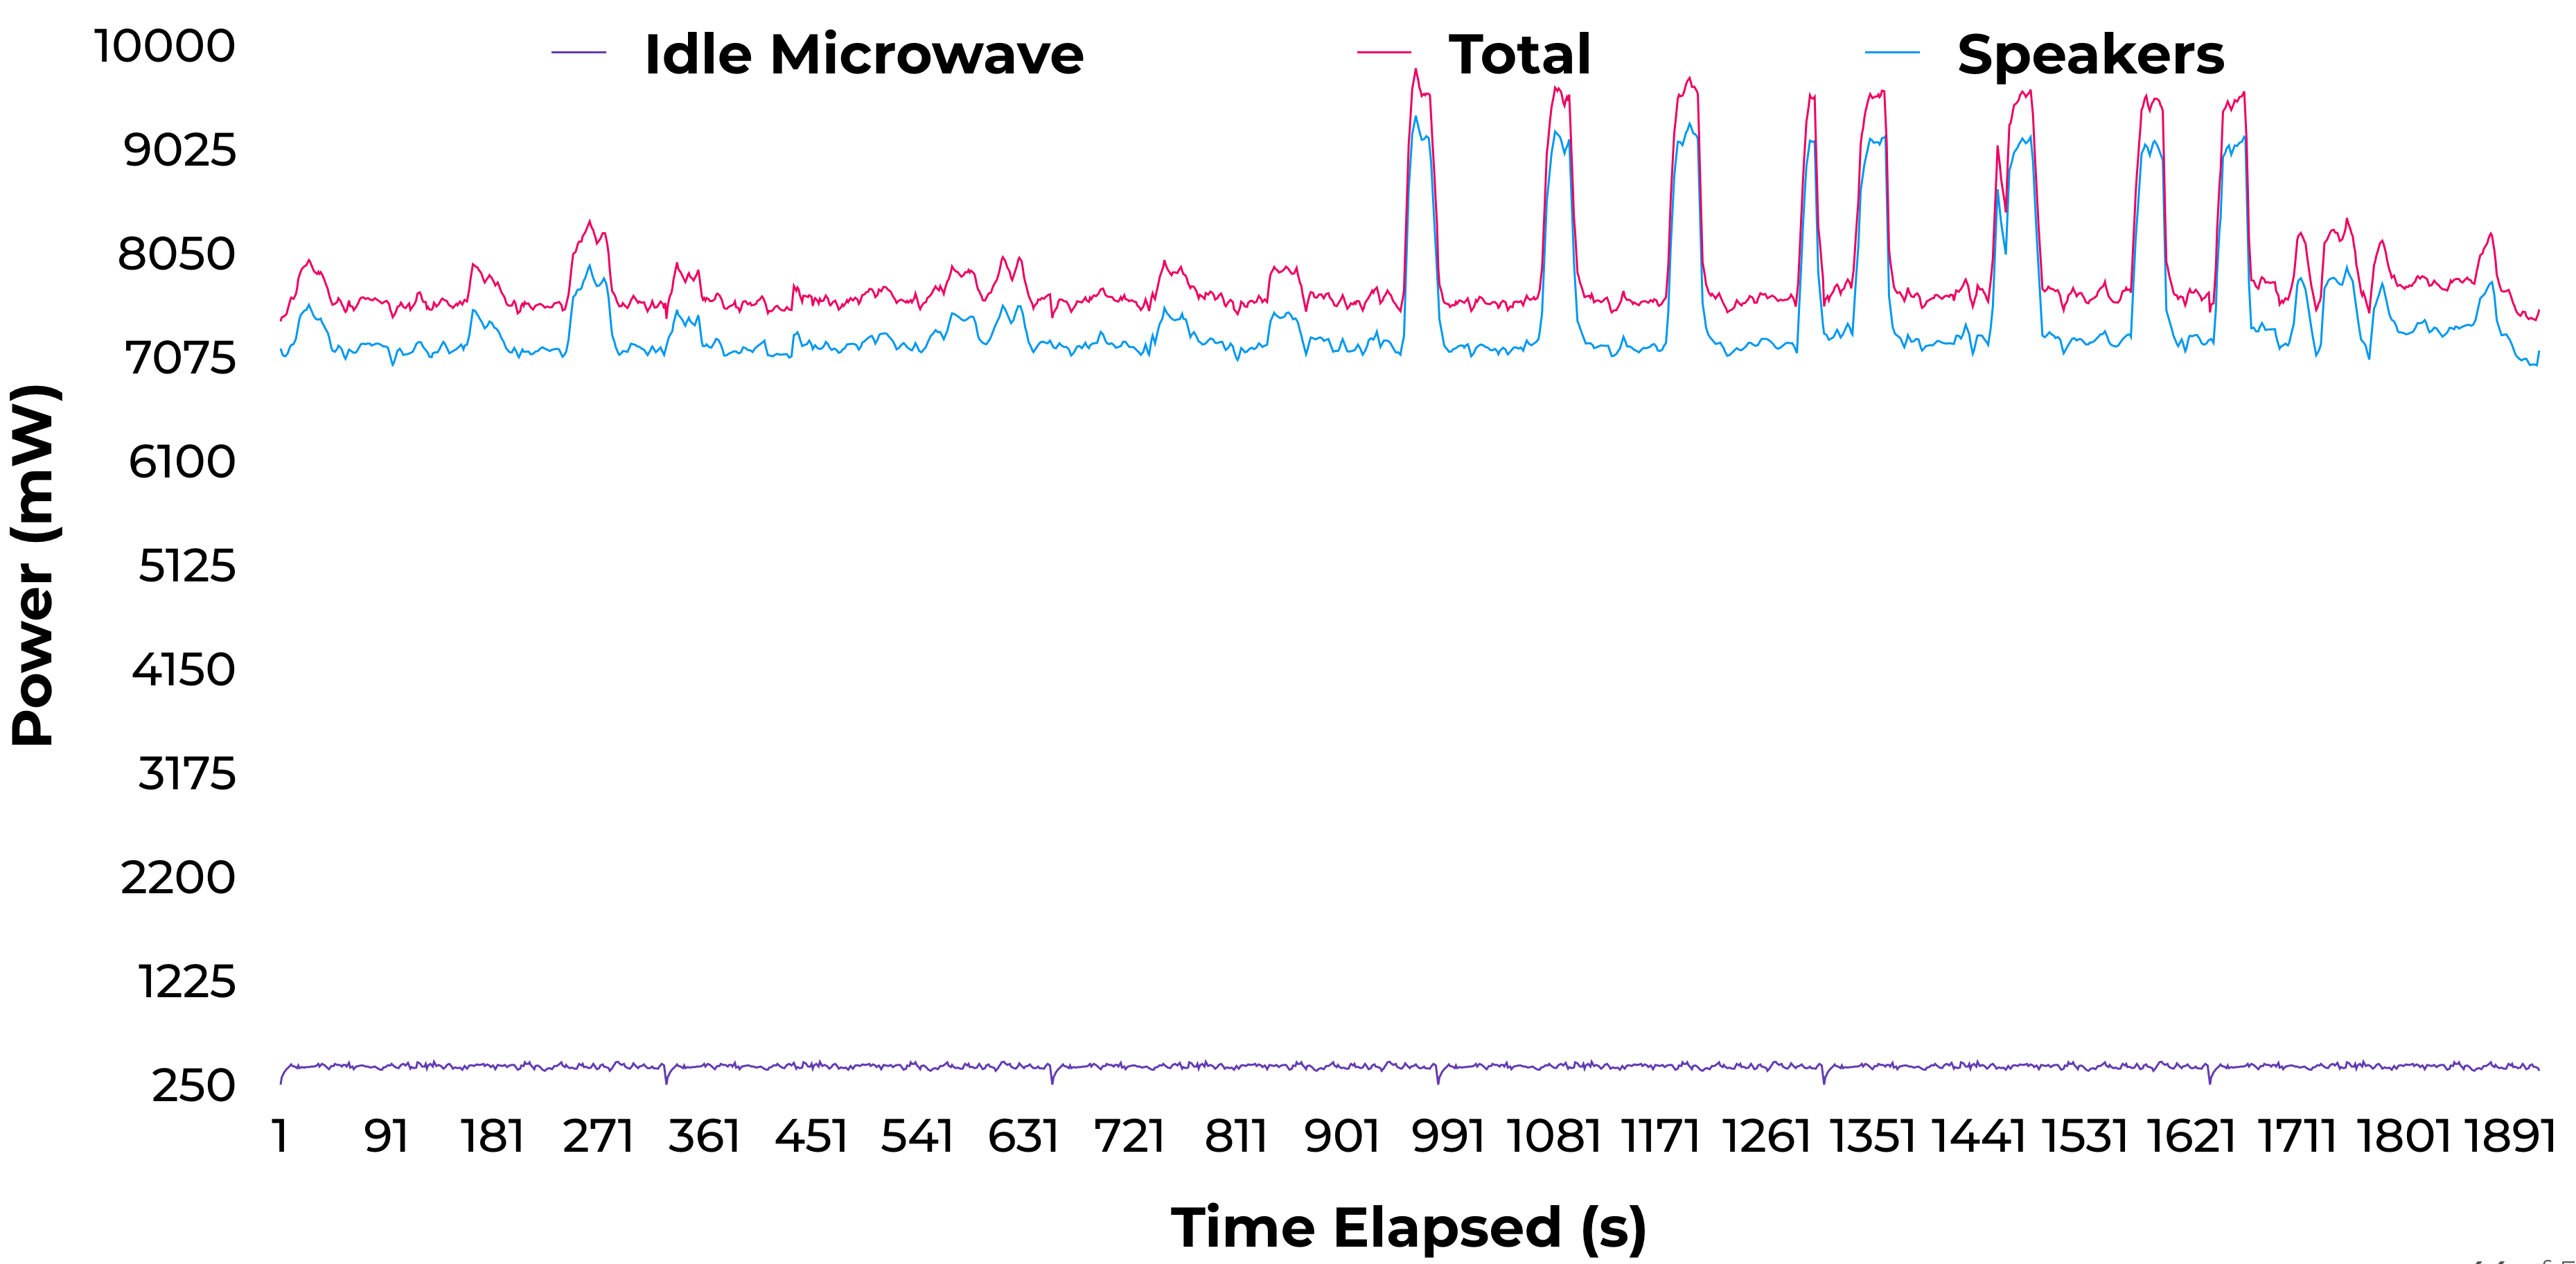
\includegraphics[width=1\textwidth]{figures/idleuWaveNoise.png}
  \caption{Figure \ref{fig:bestBballSum} summed smart speaker power, idle microwave noise, and total power.}
  \label{fig:uWaveIdle}
\end{figure}

\begin{figure}[H]
  \centering
  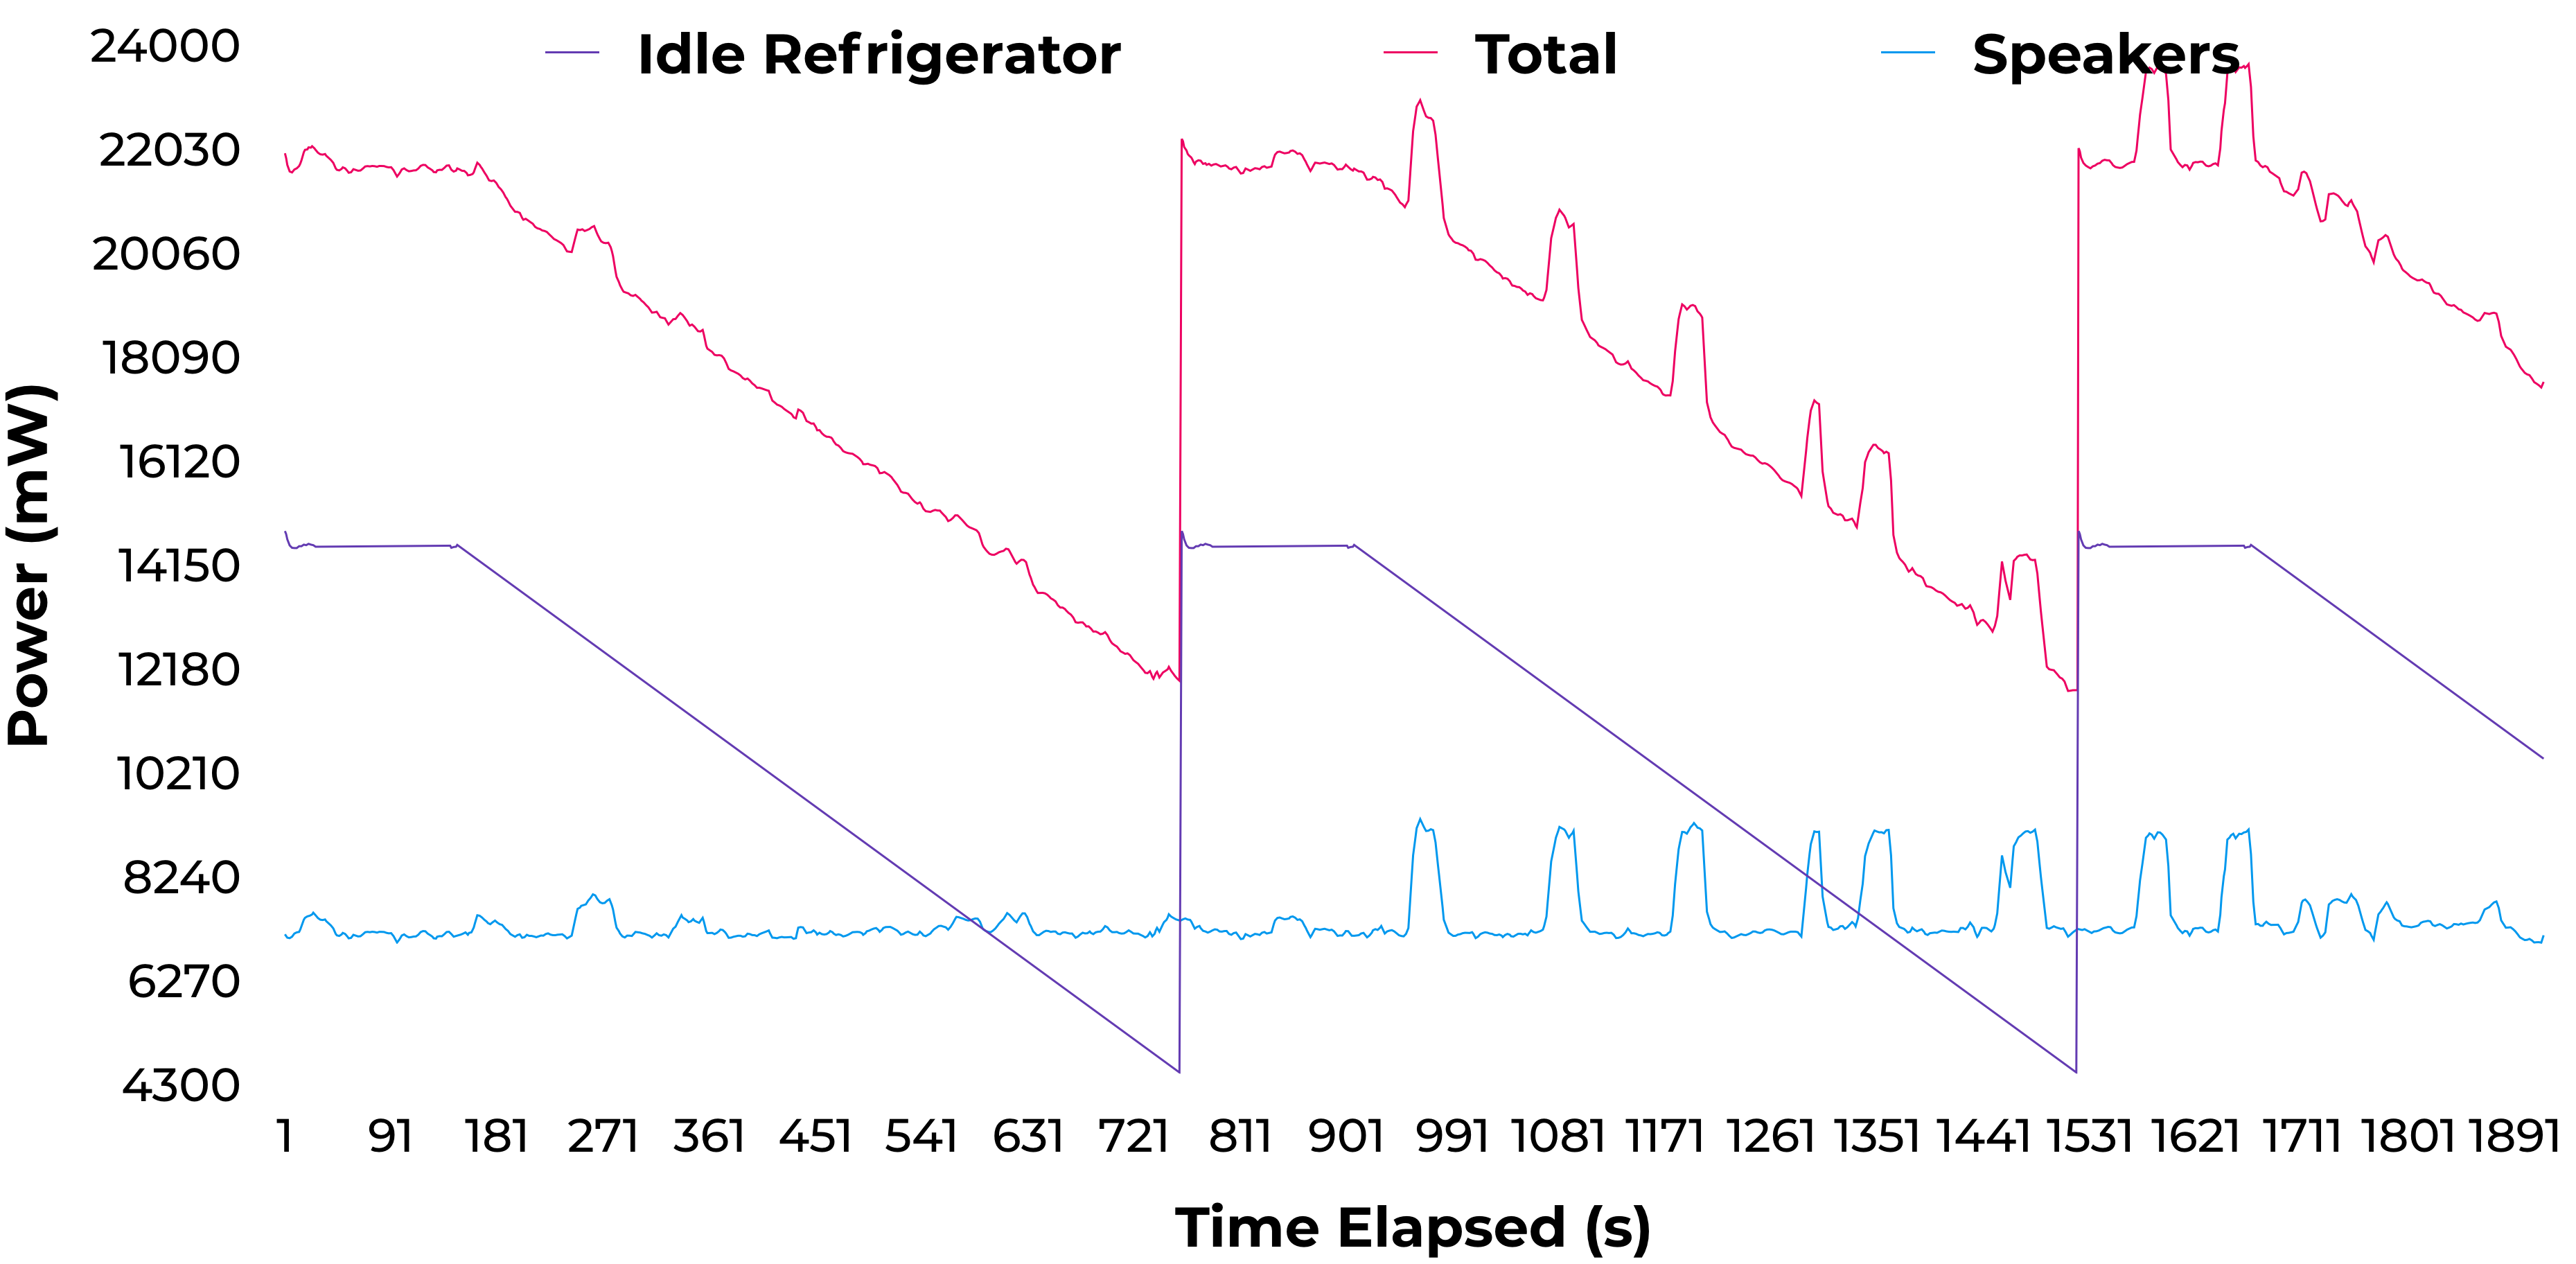
\includegraphics[width=1\textwidth]{figures/idleFridgeNoise.png}
  \caption{Figure \ref{fig:bestBballSum} summed smart speaker power, idle refrigerator noise, and total power.}
  \label{fig:fridgeIdle}
\end{figure}

\begin{figure}[H]
  \centering
  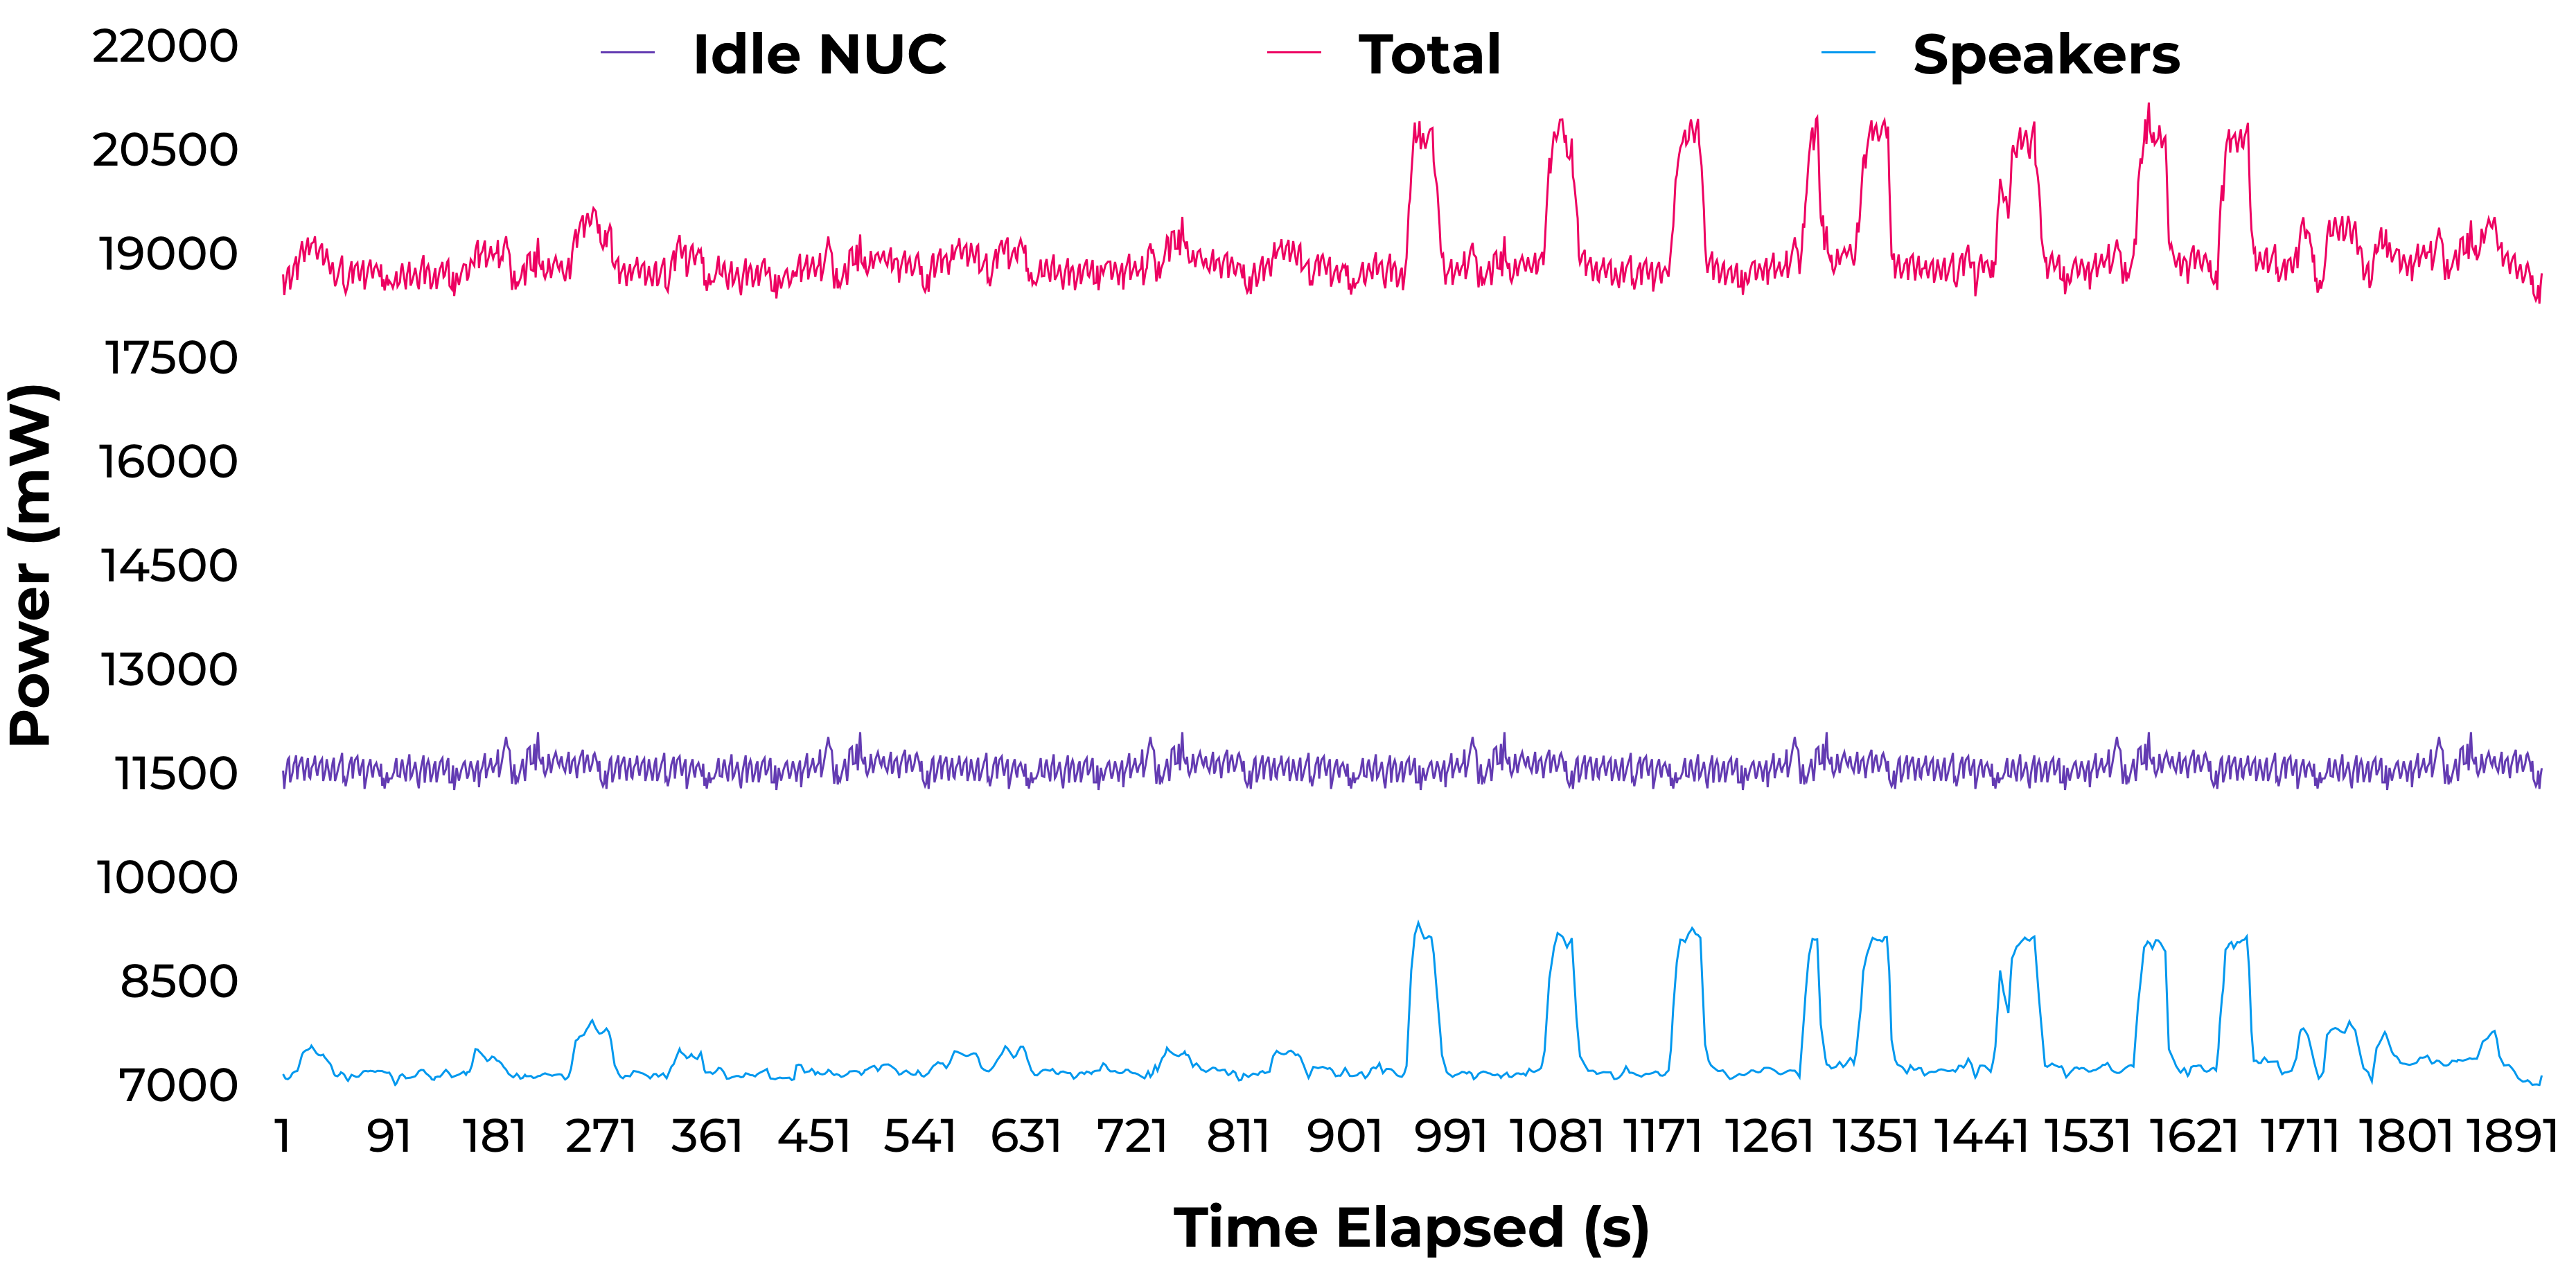
\includegraphics[width=1\textwidth]{figures/idleIntelNUCNoise.png}
  \caption{Figure \ref{fig:bestBballSum} summed smart speaker power, idle idle Intel NUC noise, and total power.}
  \label{fig:nucIdle}
\end{figure}

\begin{figure}[H]
    \centering
    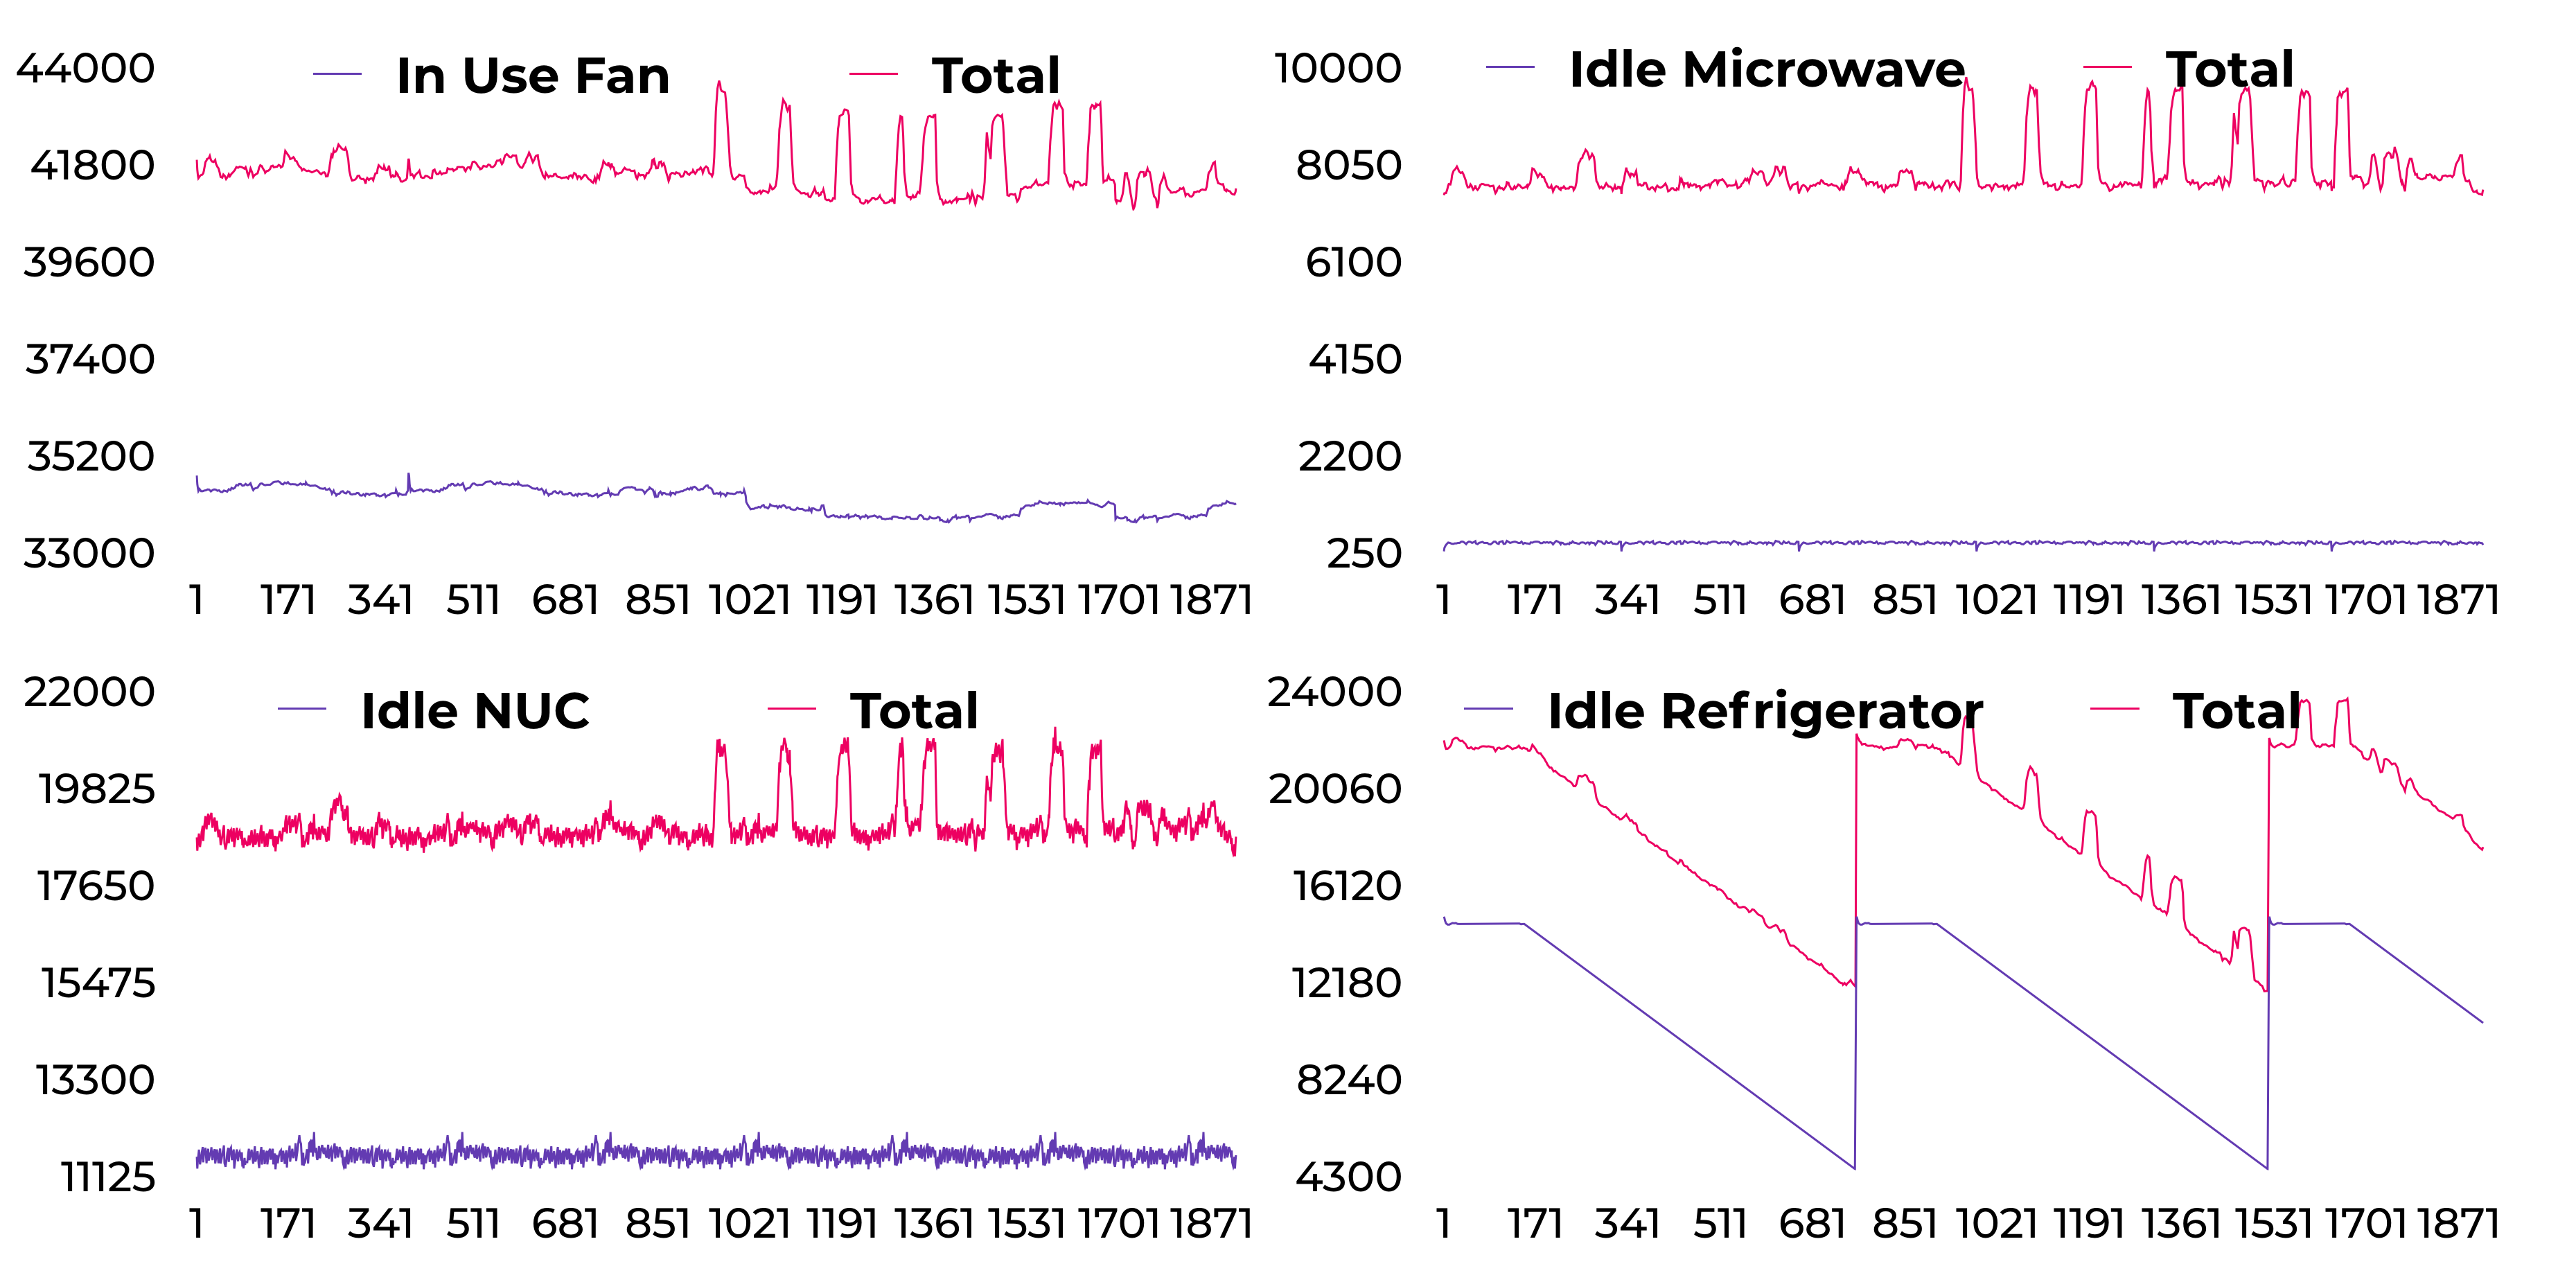
\includegraphics[width=1\textwidth]{figures/allIdleNoise.png}
    \caption{\ref{fig:fanIdle}, \ref{fig:uWaveIdle}, \ref{fig:fridgeIdle}, and \ref{fig:nucIdle} figures zoomed in}
    \label{fig:allIdleNoise}
  \end{figure}

In Figures \ref{fig:fanIdle}, \ref{fig:uWaveIdle}, \ref{fig:fridgeIdle}, and \ref{fig:nucIdle}, the power spikes from the smart speakers can still be seen. The Echo Dot power spikes are still visible in the red trace for each graph. The power spikes for the Google Home and Eufy Genie are less visible but can still be seen. Especially when zoomed in as shown in Figure \ref{fig:allIdleNoise}.

\begin{figure}[H]
  \centering
  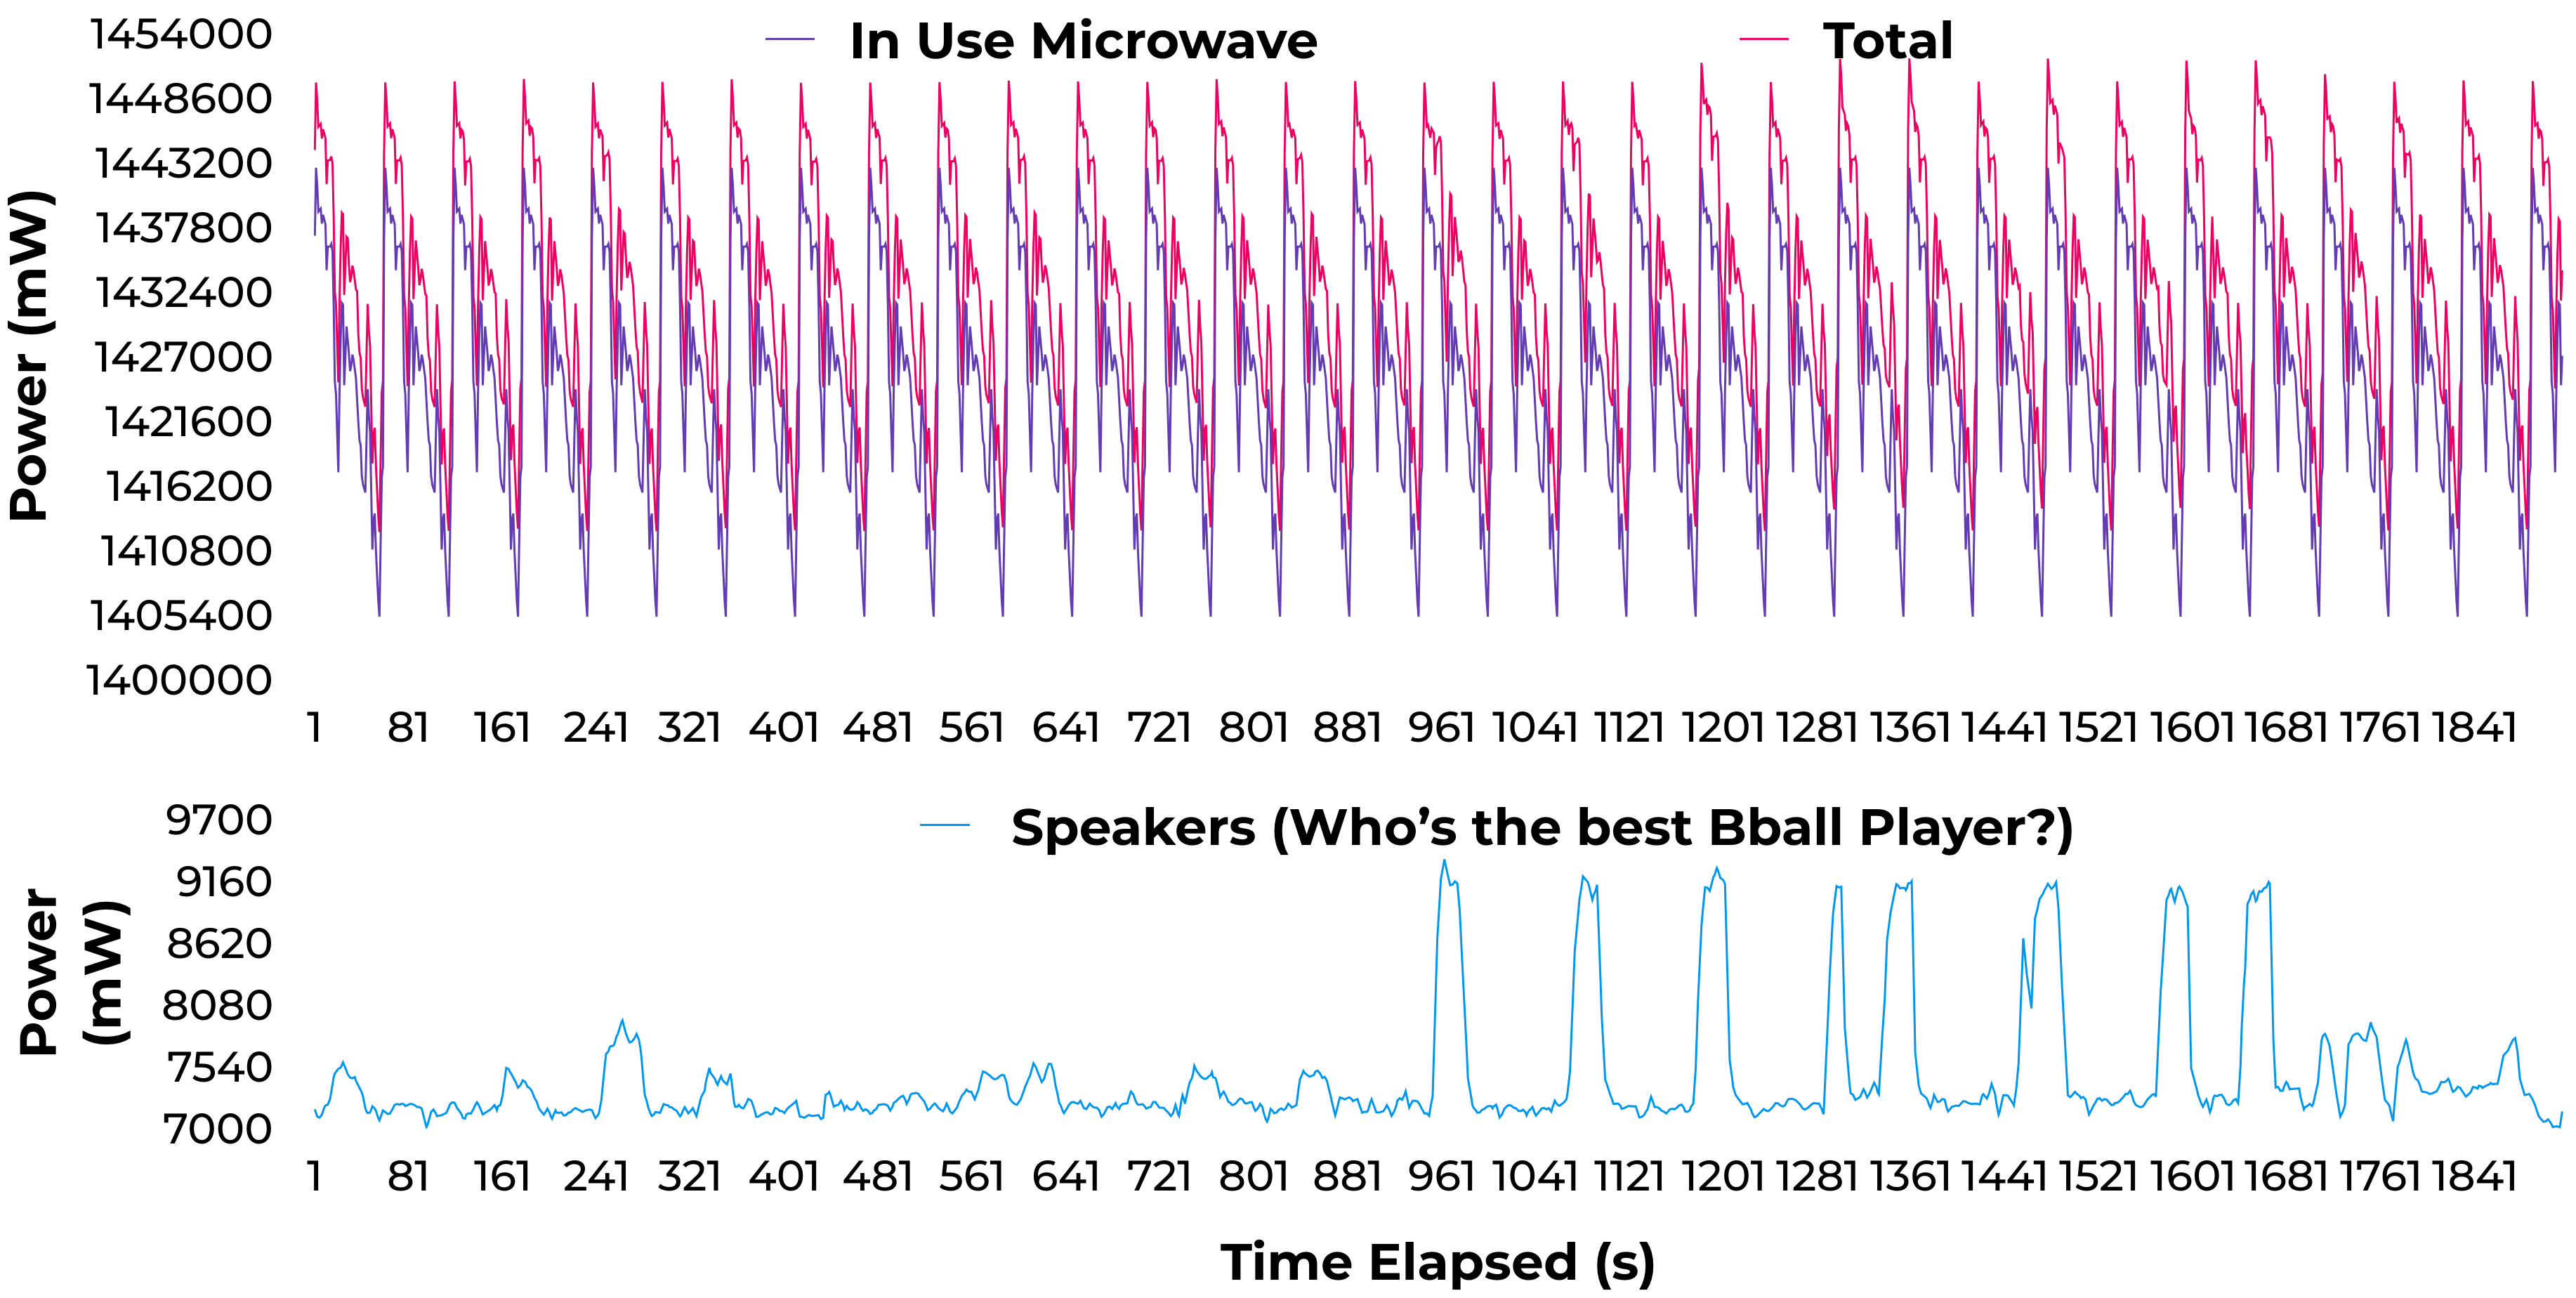
\includegraphics[width=1\textwidth]{figures/inUseuWaveNoiseSeperate.png}
  \caption{In use Microwave with Figure \ref{fig:bestBballSum} summed smart speaker power separately.}
  \label{fig:uWaveInUseSeperate}
\end{figure}

\begin{figure}[H]
  \centering
  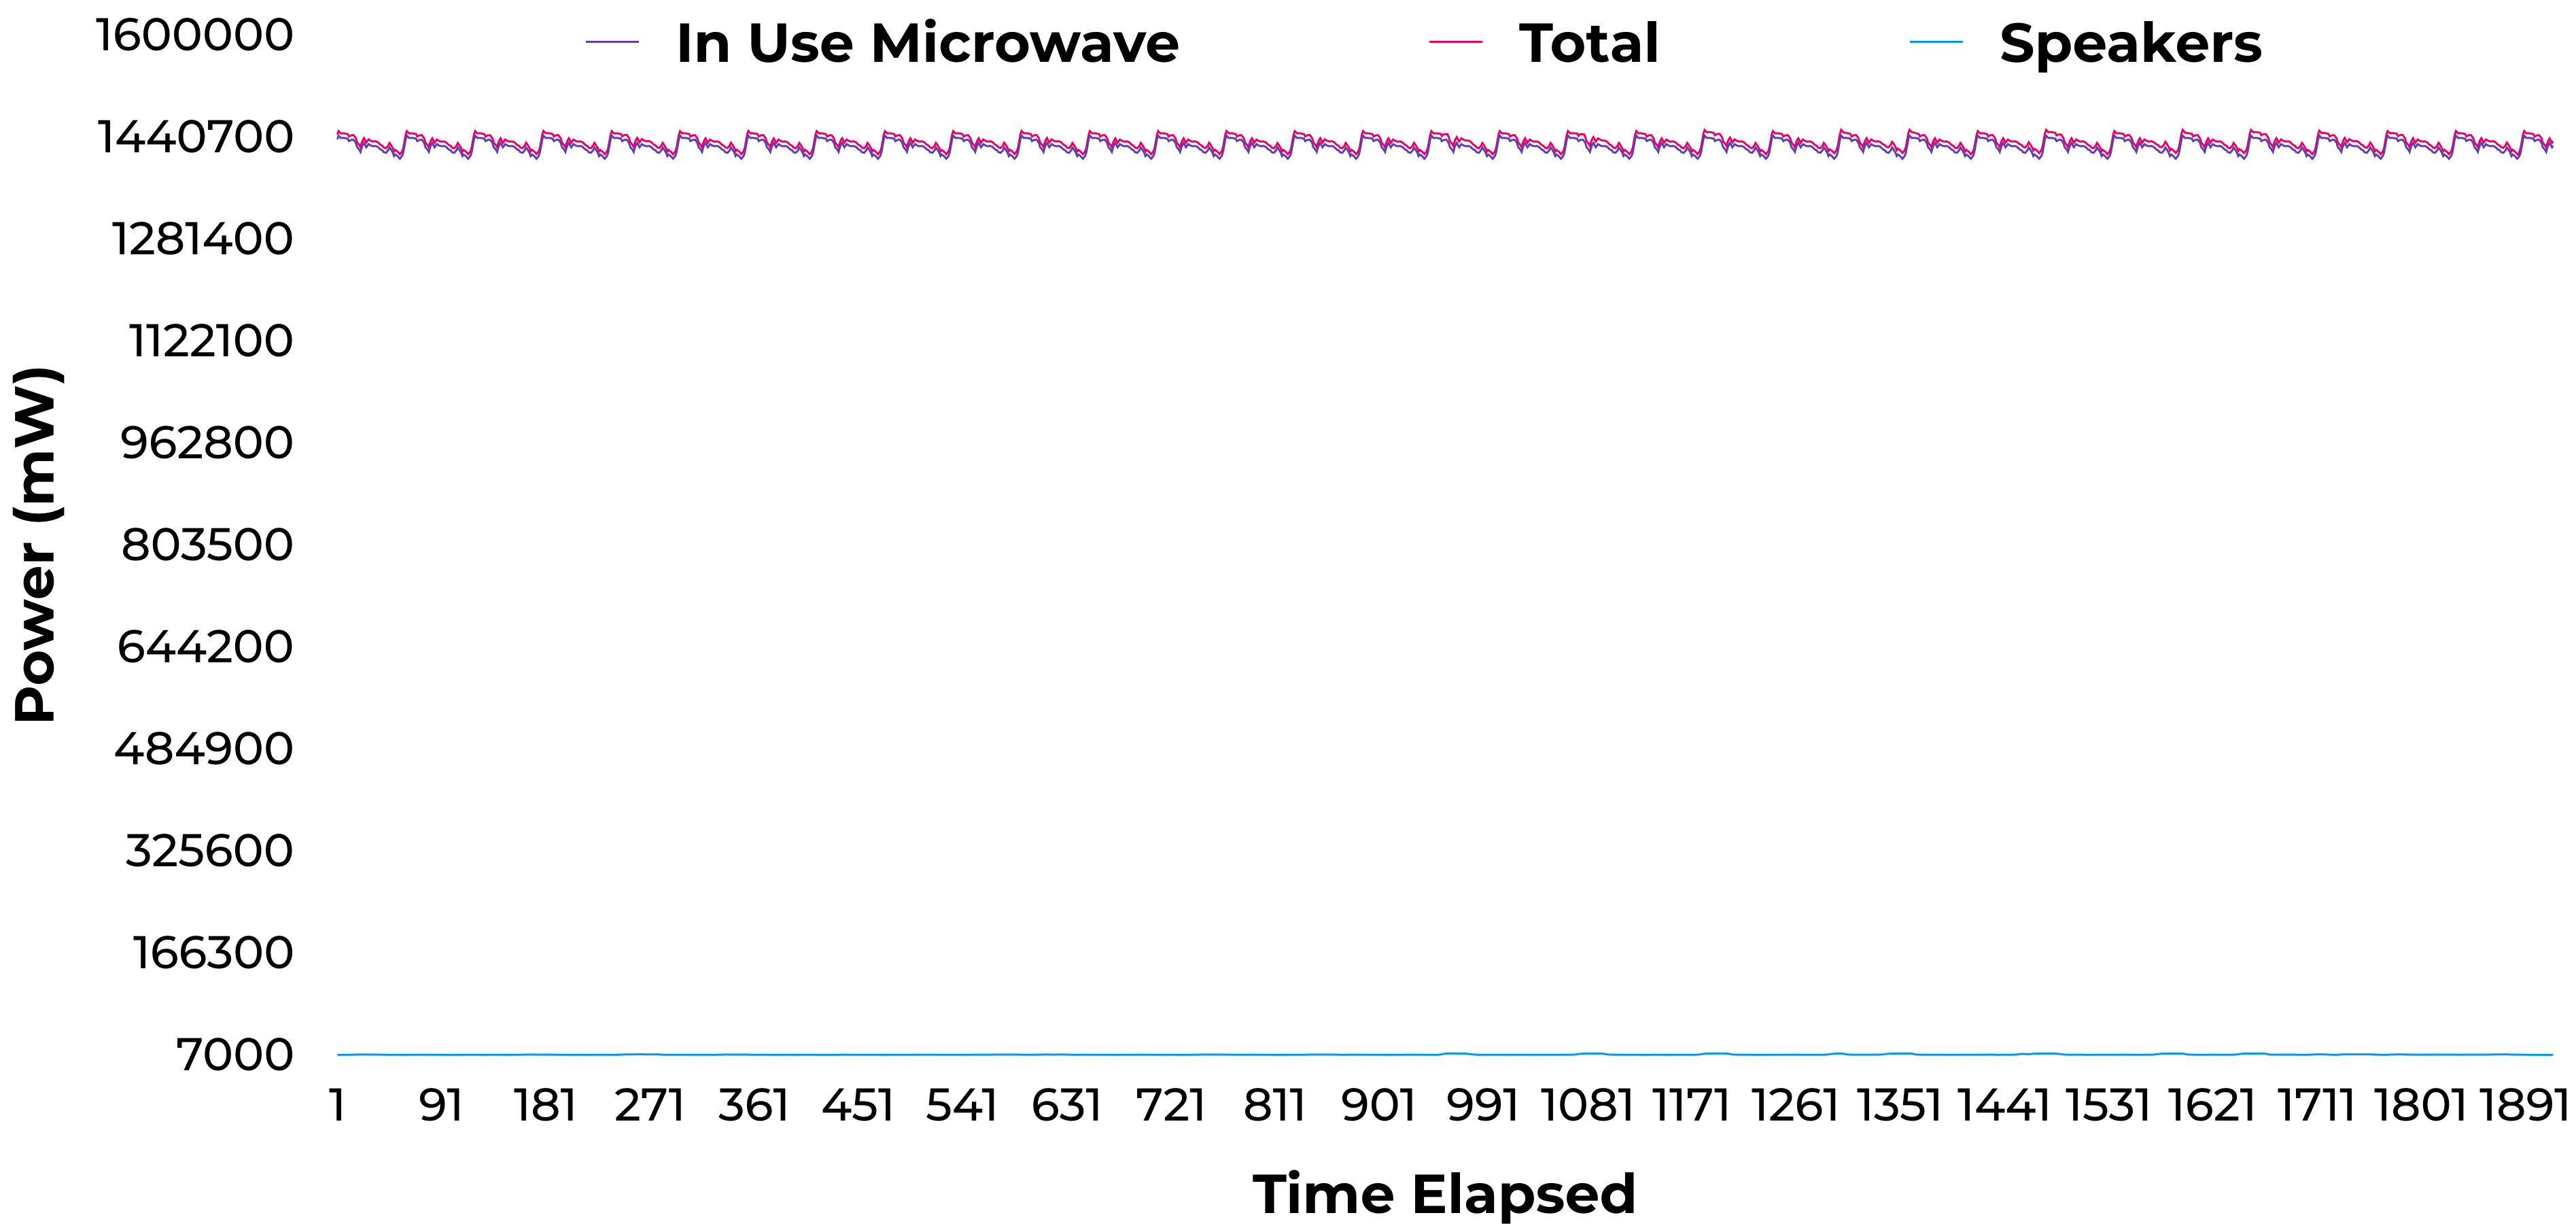
\includegraphics[width=1\textwidth]{figures/inUseuWaveNoise.png}
  \caption{In use Microwave with Figure \ref{fig:bestBballSum} summed smart speaker power.}
  \label{fig:uWaveInUse}
\end{figure}

\begin{figure}[H]
  \centering
  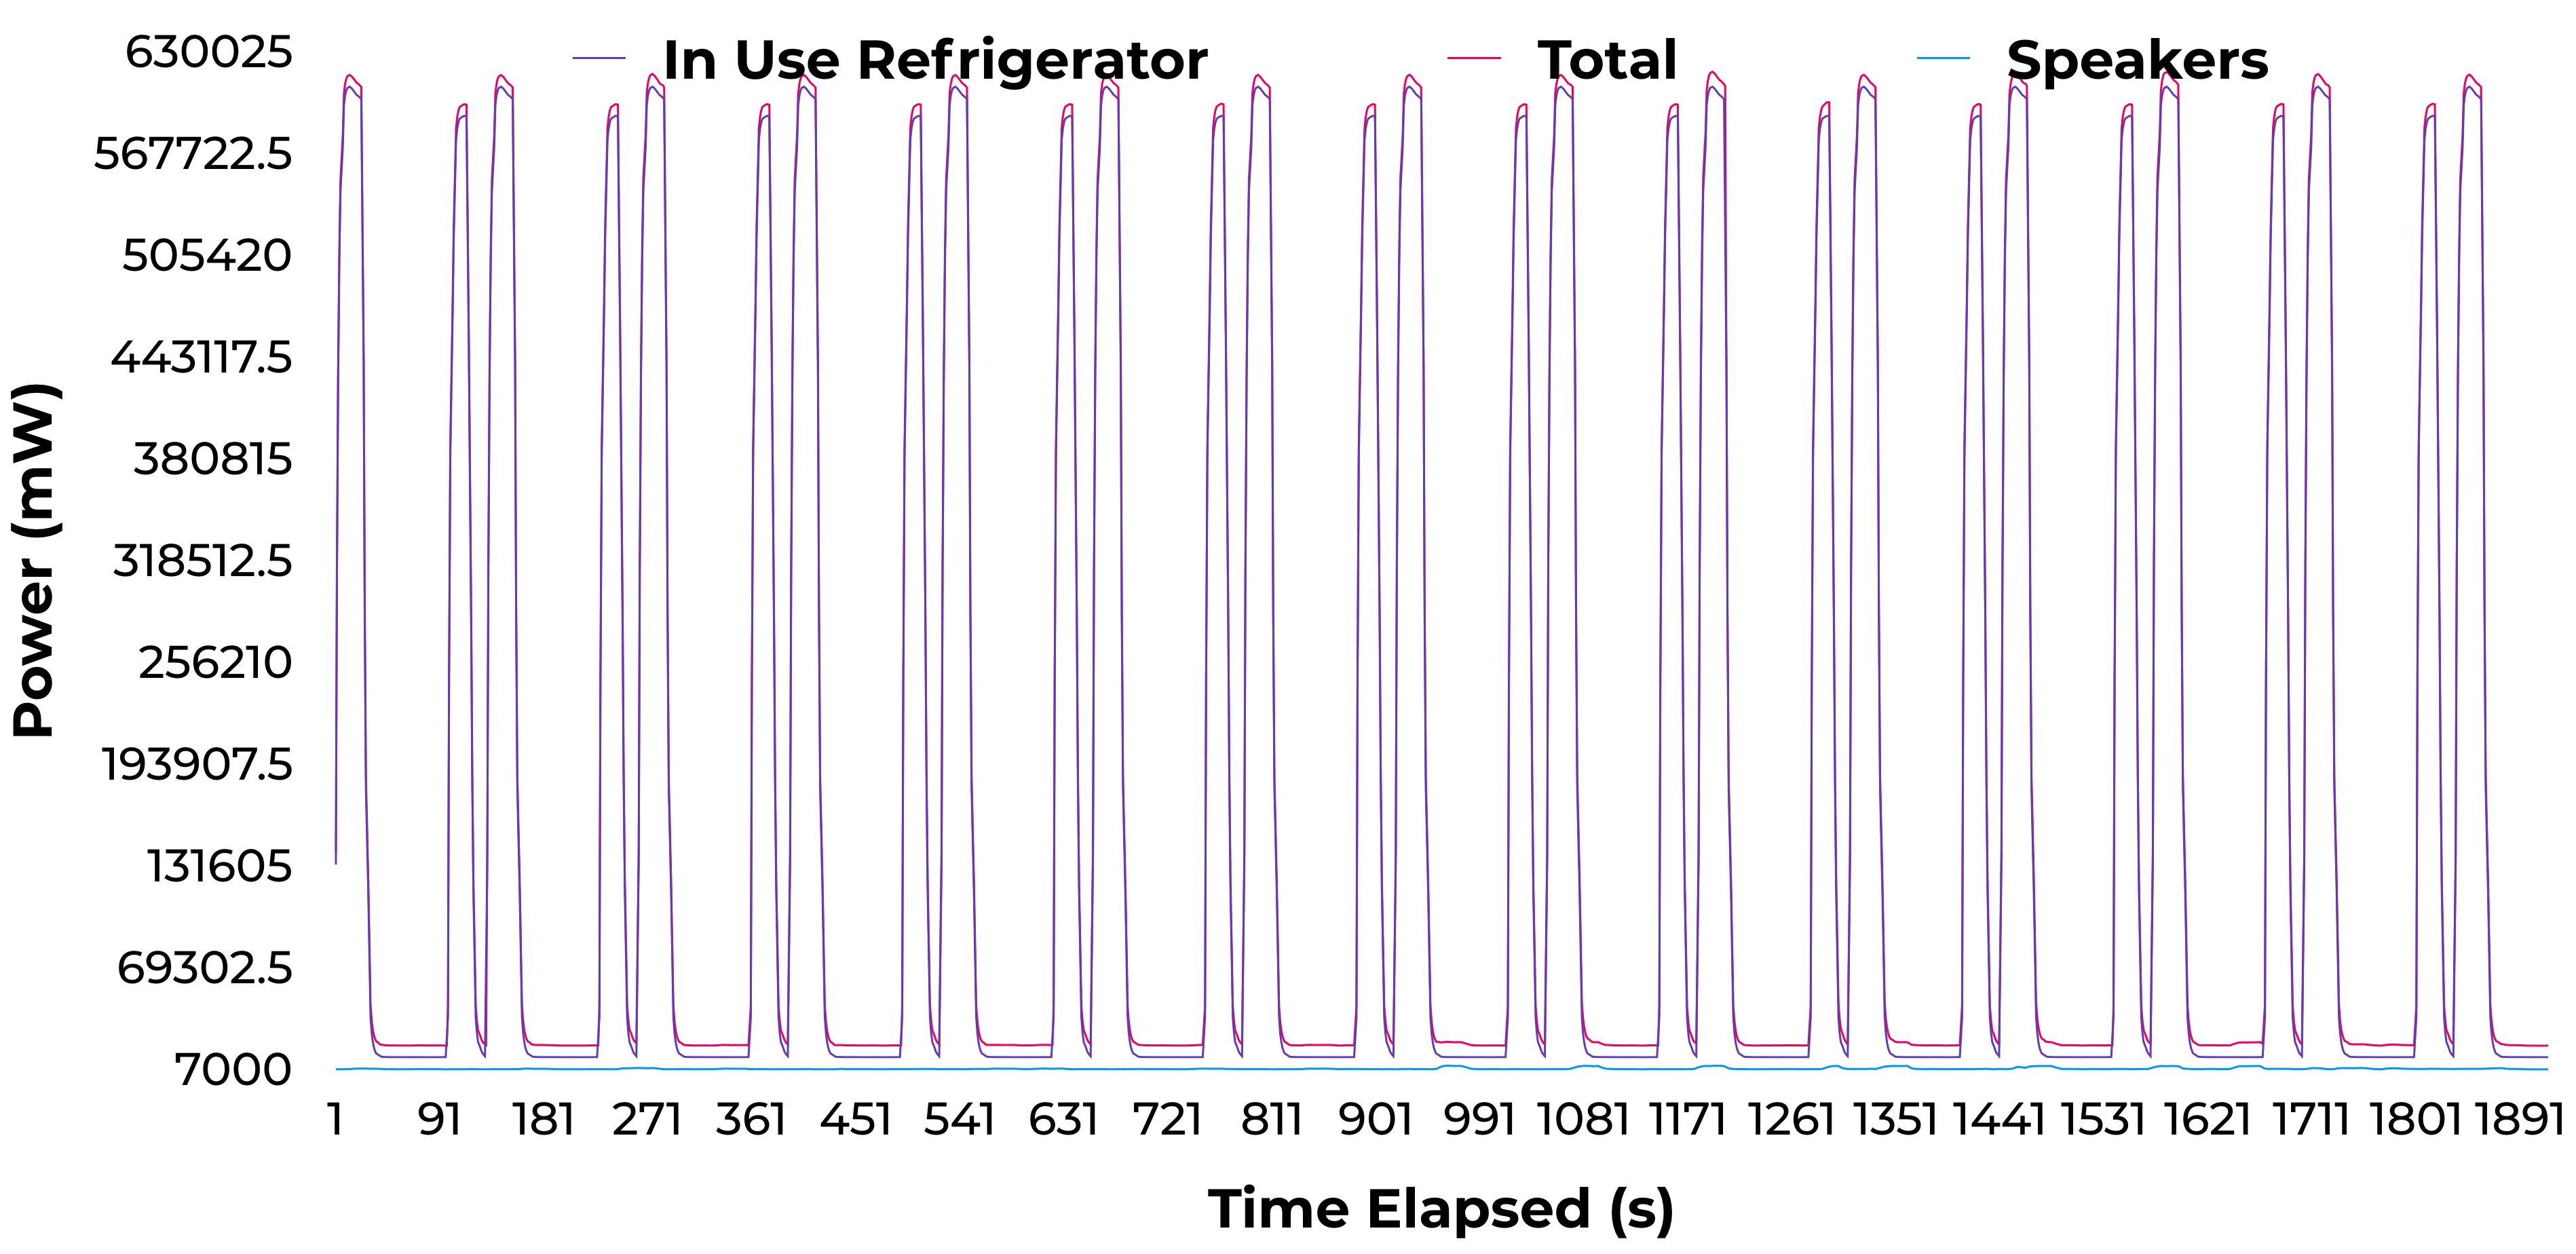
\includegraphics[width=1\textwidth]{figures/inUseFridgeNoise.png}
  \caption{Fridge in the middle of cooling with Figure \ref{fig:bestBballSum} summed smart speaker power.}
  \label{fig:fridgeInUse}
\end{figure}

\begin{figure}[H]
  \centering
  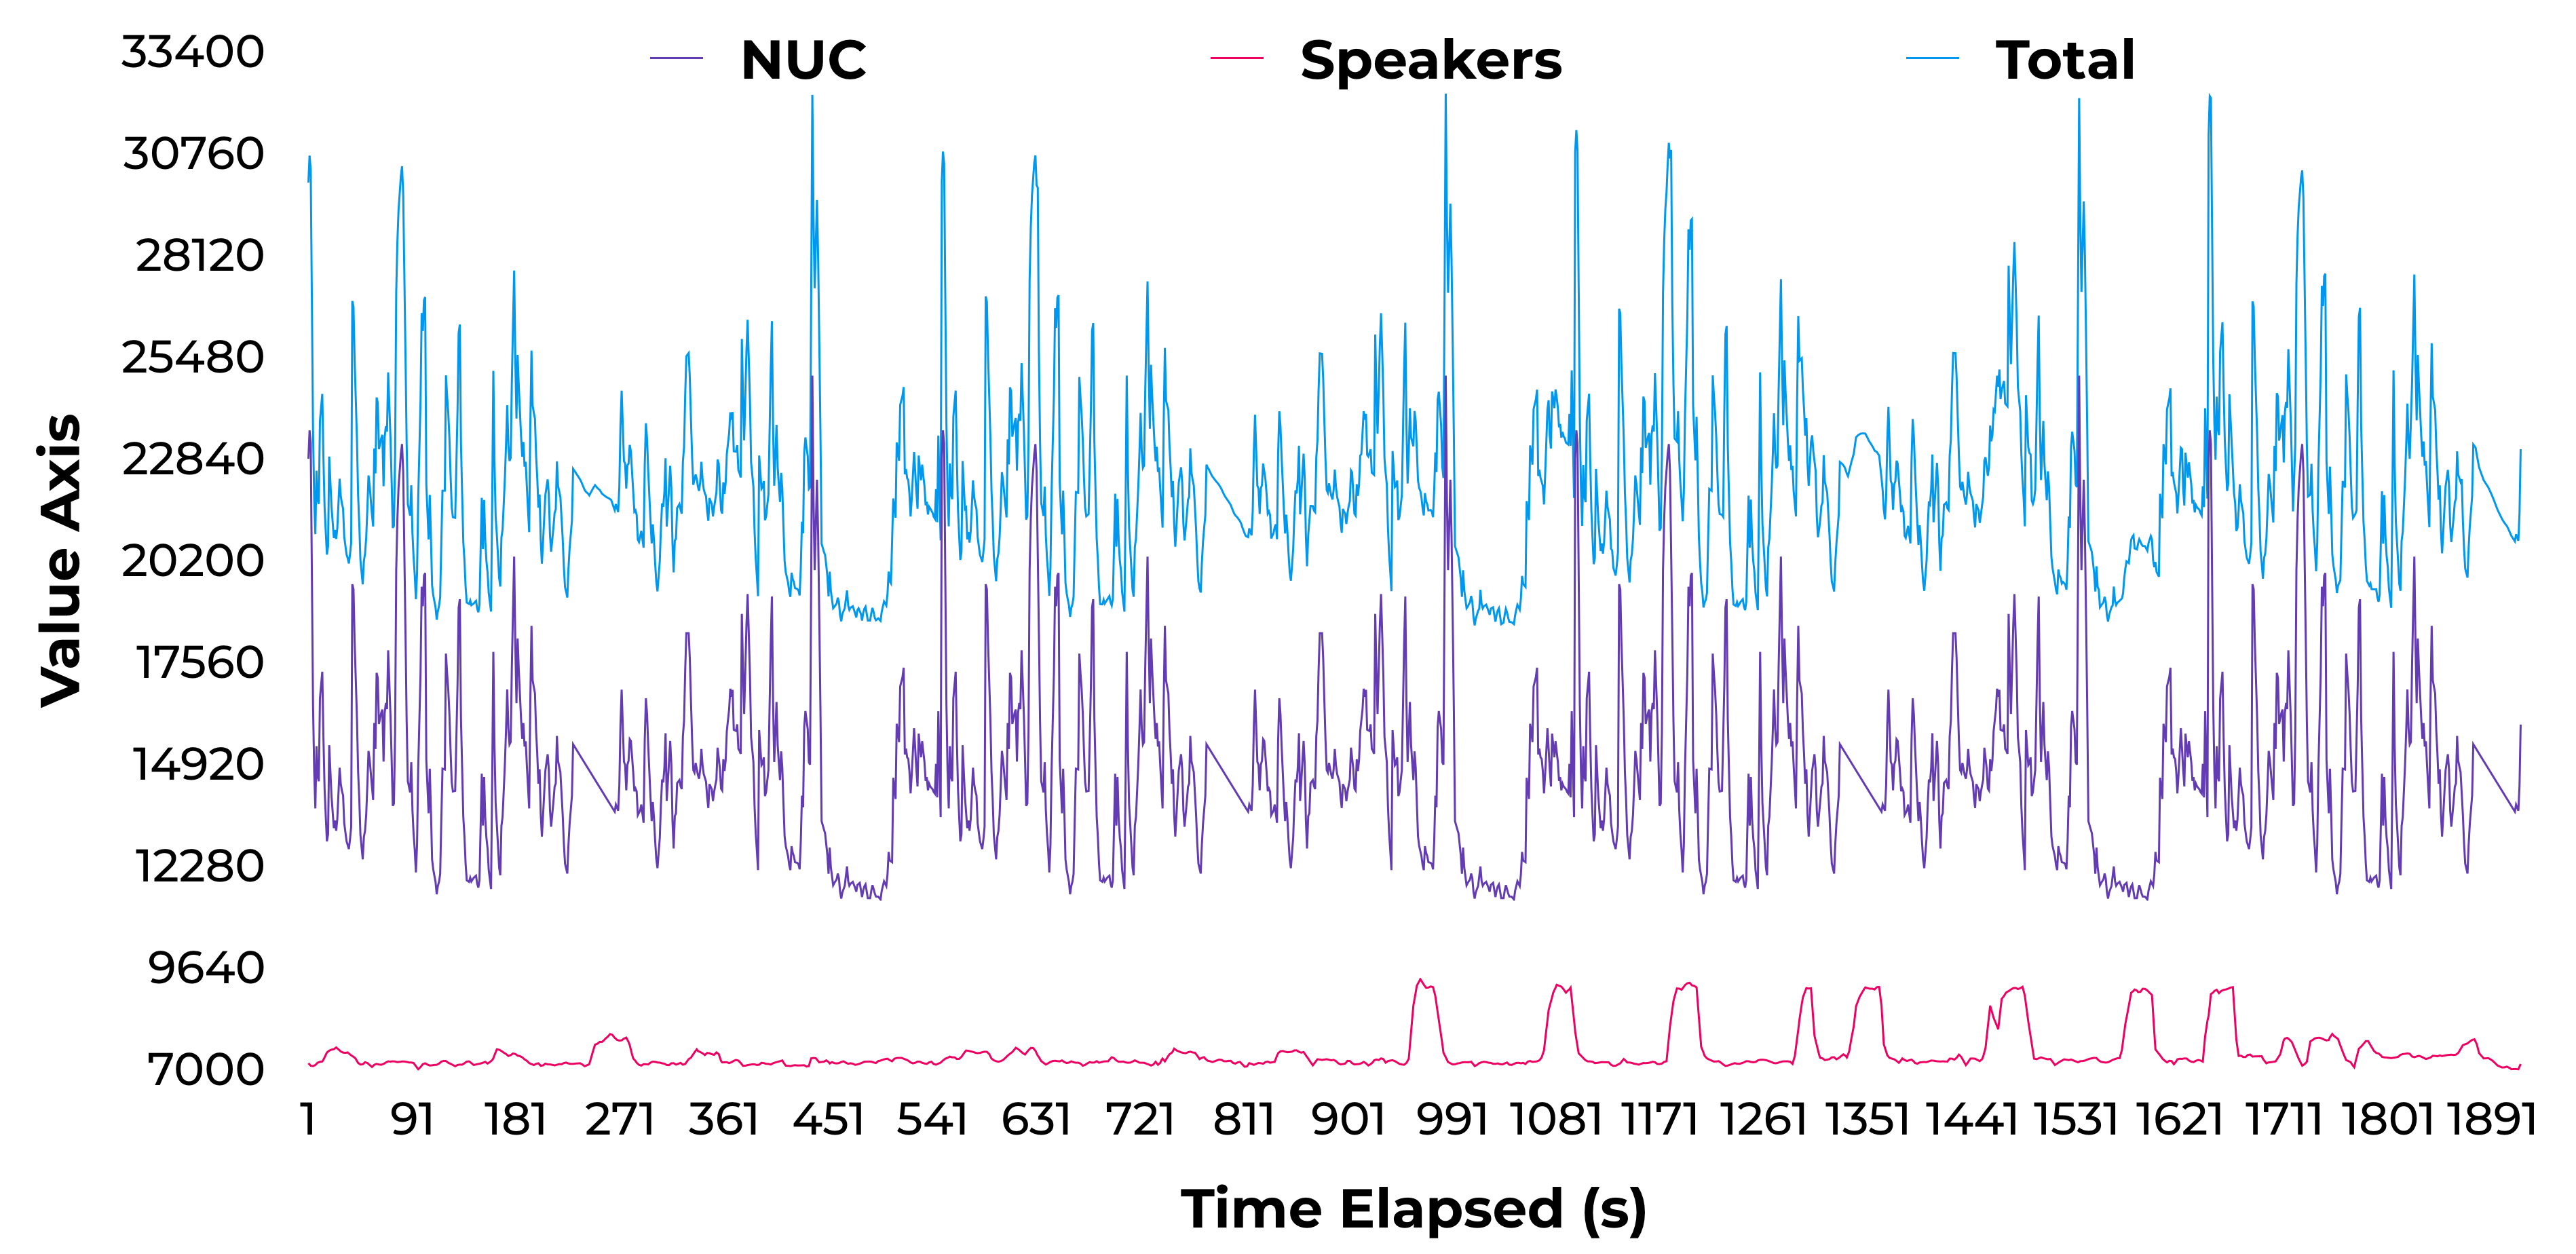
\includegraphics[width=1\textwidth]{figures/inUseNUCNoise.png}
  \caption{PC in use with Figure \ref{fig:bestBballSum} summed smart speaker power.}
  \label{fig:nucInUse}
\end{figure}

Figures \ref{fig:fanIdle} - \ref{fig:nucInUse} show that it is possible to determine that a smart speaker is in use from visual examination of power spikes even in the presence of noise. If the noise within the house is stable, the power spikes are shifted up as shown in Figure \ref{fig:fanIdle}. If the noise within the house is low power then, the spikes visually overpower the noise, as shown in Figure \ref{fig:nucIdle}.

But if the noise within the house is considerable in magnitude such as the microwave or fridge while in use \ref{fig:uWaveInUse} \ref{fig:fridgeInUse}, this noise will squash the power spikes from the smart speakers. The spikes can no longer be seen, even when zoomed in, as shown in Figure \ref{fig:uWaveInUseSeperate}. The smart speaker spikes also disappear if the noise of a device is on the same or a larger magnitude than the power spikes, as shown in Figure \ref{fig:nucInUse}. The power spikes can still be seen in the sum graph for this figure, but it is impossible to visually differentiate between a power spike from a speaker and the introduced noise without knowing the original smart speaker graph.

These two cases vary depending on the household. If many battery power devices such as laptops (replacing the NUC) or phones are used, then it may still be possible to determine the power spikes visually. If high power devices such as the microwave or fridge are not in use often, then the smart speaker spikes may be visually correlated. But if a household has many devices plugged into an outlet for power, then the smart speaker power spikes are likely to disappear from the additive noise of all the devices. Regardless, there are privacy implications in a household's power line. With easy, direct, access to a household's power line \cite{griffith_2017}, someone could determine the device in use within a household.